\documentclass[11pt]{article}

\usepackage[review]{acl}
\usepackage{times}
\usepackage{latexsym}
\usepackage[T1]{fontenc}
\usepackage[utf8]{inputenc}
\usepackage{microtype}
\usepackage{inconsolata}
\usepackage{booktabs}
\usepackage{graphicx}
\usepackage{array}
\usepackage{tabularx}
\usepackage{enumitem}
\usepackage{placeins}
\usepackage{amsmath}
\usepackage{amsfonts}
\usepackage{amssymb}
\usepackage{forest}
\usepackage{tikz}
\usepackage{titletoc}
\usetikzlibrary{arrows.meta,calc,positioning,fit,backgrounds}
% Generated by scripts/analyze_controlled_model_judges_v2.py. Do not edit.
\newcommand{\CMJmodels}{28}
\newcommand{\CMJpassing}{25}
\newcommand{\CMJfailing}{3}
\newcommand{\CMJdraws}{1,200}
\newcommand{\CMJCtwoPooled}{+3.1}
\newcommand{\CMJCtwoLow}{+0.7}
\newcommand{\CMJCtwoHigh}{+5.5}
\newcommand{\CMJCtwoP}{.013}
\newcommand{\CMJCtwoIsq}{98}
\newcommand{\CMJCfivePooled}{+0.1}
\newcommand{\CMJCfiveLow}{-1.3}
\newcommand{\CMJCfiveHigh}{+1.5}
\newcommand{\CMJCfiveP}{.933}
\newcommand{\CMJCfiveIsq}{97}
\newcommand{\CMJProbePooled}{-0.4}
\newcommand{\CMJProbeLow}{-1.0}
\newcommand{\CMJProbeHigh}{+0.3}
\newcommand{\CMJProbeP}{.256}
\newcommand{\CMJProbeIsq}{90}
\newcommand{\CMJprobeMin}{41.9}
\newcommand{\CMJprobeMax}{99.8}

% Generated by scripts/build_revision_macros.py -- do not edit by hand.
\newcommand{\LedgerStated}{8}
\newcommand{\LedgerStatedUndef}{4}
\newcommand{\LedgerStatedNarrow}{2}
\newcommand{\LedgerStatedSurv}{2}
\newcommand{\LedgerInvited}{4}
\newcommand{\LedgerInvitedUndef}{3}
\newcommand{\LedgerCrossPaper}{12}
\newcommand{\VerifChecks}{102}
\newcommand{\TierPanelN}{9}
\newcommand{\TierNew}{6}
\newcommand{\TierFrontierVerdict}{0.54}
\newcommand{\TierFrontierVerdictK}{0.31}
\newcommand{\TierFrontierDevs}{3}
\newcommand{\TierSmallVerdictK}{0.00}
\newcommand{\TierSubmittedVerdictK}{0.14}
\newcommand{\TierSameDevVerdict}{0.56}
\newcommand{\TierSameDevVerdictK}{0.35}
\newcommand{\TierSameDevGoogleK}{0.29}
\newcommand{\TierSameDevOpenAIK}{0.20}
\newcommand{\TierPairSameDevSameTier}{0.28}
\newcommand{\TierPairSameDevDiffTier}{0.17}
\newcommand{\TierPairDiffDevSameTier}{0.13}
\newcommand{\TierPairDiffDevDiffTier}{0.06}
\newcommand{\TierCompFFCross}{+0.17}
\newcommand{\TierCompFFCrossLo}{+0.00}
\newcommand{\TierCompFFCrossHi}{+0.32}
\newcommand{\TierCompFFSame}{+0.28}
\newcommand{\TierCompSSCross}{-0.03}
\newcommand{\TierDevDiff}{+0.11}
\newcommand{\TierTierDiff}{+0.06}
\newcommand{\TierDevP}{0.004}
\newcommand{\TierTierP}{0.19}
\newcommand{\TierDevRand}{280}
\newcommand{\TierTierRand}{84}
\newcommand{\TierPairDiff}{+0.11}
\newcommand{\TierPairP}{0.07}
\newcommand{\TierPairRand}{15}
\newcommand{\TierDevBootShare}{94}
\newcommand{\TierDevBootCI}{[-0.02, +0.26]}
\newcommand{\TierFrontSame}{+0.28}
\newcommand{\TierFrontCross}{+0.17}
\newcommand{\TierFrontCrossLo}{+0.00}
\newcommand{\TierFrontCrossHi}{+0.32}
\newcommand{\TierFrontCrossBeats}{6}
\newcommand{\TierCommonItems}{843}
\newcommand{\TierAllItems}{1,680}
\newcommand{\TierFrontierVerdictKAll}{0.51}
\newcommand{\TierSubmittedVerdictKAll}{0.33}
\newcommand{\TierNPairs}{36}
\newcommand{\TierSurvivesLo}{18}
\newcommand{\TierSurvivesHi}{78}
\newcommand{\FrameCandidates}{1,703}
\newcommand{\FrameFiles}{171}
\newcommand{\FrameScreened}{259}
\newcommand{\CensusCoded}{1,690}
\newcommand{\CensusHeldout}{1,586}
\newcommand{\CensusDevSize}{133}
\newcommand{\CensusEligible}{704}
\newcommand{\CensusUnanimous}{449}
\newcommand{\CensusPapers}{103}
\newcommand{\CensusUndefined}{221}
\newcommand{\CensusNarrows}{1}
\newcommand{\CensusSurvives}{384}
\newcommand{\CensusNoMajority}{98}
\newcommand{\CensusKappaVerdict}{0.06}
\newcommand{\CensusKappaElig}{0.51}
\newcommand{\CensusAcVerdict}{0.22}
\newcommand{\CensusAcElig}{0.51}
\newcommand{\CensusJudges}{3}
\newcommand{\CensusCodings}{5,070}
\newcommand{\CensusObsElig}{0.75}
\newcommand{\CensusQuoteRate}{87}
\newcommand{\CensusGapPct}{57}
\newcommand{\DecProv}{0.79}
\newcommand{\DecProvCI}{[0.73, 0.88]}
\newcommand{\DecProvPapers}{99}
\newcommand{\DecProvK}{0.55}
\newcommand{\DecElig}{0.51}
\newcommand{\DecEligCI}{[0.41, 0.64]}
\newcommand{\DecEligPapers}{169}
\newcommand{\DecEligK}{0.51}
\newcommand{\DecEligM}{0.69}
\newcommand{\DecEligMCI}{[0.63, 0.79]}
\newcommand{\DecEligMK}{-0.14}
\newcommand{\DecVerdict}{0.22}
\newcommand{\DecVerdictCI}{[0.18, 0.26]}
\newcommand{\DecVerdictPapers}{103}
\newcommand{\DecVerdictK}{0.06}
\newcommand{\DecGap}{+0.57}
\newcommand{\DecGapCI}{[0.50, 0.68]}
\newcommand{\DecGapK}{+0.49}
\newcommand{\DecGapKCI}{[0.11, 0.63]}
\newcommand{\DecGapEl}{+0.47}
\newcommand{\DecGapElCI}{[0.40, 0.57]}
\newcommand{\DecGapElK}{-0.20}
\newcommand{\DecGapElKCI}{[-0.24, -0.11]}
\newcommand{\DecDraws}{2,000}
\newcommand{\DecCoordMin}{0.38}
\newcommand{\DecCoordMax}{0.72}
\newcommand{\DecCoordKMin}{-0.11}
\newcommand{\DecCoordKMax}{0.19}
\newcommand{\ProvClassified}{610}
\newcommand{\ProvCoded}{658}
\newcommand{\ProvUnclassified}{48}
\newcommand{\ProvNoMajority}{4}
\newcommand{\ProvTransported}{77}
\newcommand{\ProvReimplemented}{533}
\newcommand{\ProvUnclear}{44}
\newcommand{\ProvReimplPct}{87.4}
\newcommand{\ProvKappa}{0.55}
\newcommand{\ProvAc}{0.79}
\newcommand{\ProvObs}{0.83}
\newcommand{\ProvTransFail}{67.5}
\newcommand{\ProvTransPapers}{9}
\newcommand{\ProvReimplPapers}{84}
\newcommand{\ProvTransLargest}{76}
\newcommand{\ProvTransLOO}{[67, 85]}
\newcommand{\ProvReimplLOO}{[27, 29]}
\newcommand{\ProvTransFailCI}{[25, 89]}
\newcommand{\ProvReimplFail}{25.0}
\newcommand{\ProvReimplFailCI}{[22, 34]}
\newcommand{\ProvTransN}{77}
\newcommand{\ProvReimplN}{533}
\newcommand{\ProvTransFailN}{52}
\newcommand{\ProvReimplFailN}{133}
\newcommand{\SigmaMin}{0.31}
\newcommand{\SigmaMax}{0.78}
\newcommand{\SigmaPanelReviewers}{28}
\newcommand{\SigmaPanel}{0.54}
\newcommand{\SigmaCensus}{0.38}
\newcommand{\SigmaCensusCI}{[0.18, 0.51]}
\newcommand{\SigmaCensusRev}{9}
\newcommand{\SigmaInstrument}{0.38}
\newcommand{\SigmaInstrumentCI}{[0.12, 0.48]}
\newcommand{\SigmaHumanCorpora}{5}
\newcommand{\SigmaHumanMedian}{0.46}
\newcommand{\CMJCtwoPIlow}{-9.8}
\newcommand{\CMJCtwoPIhigh}{+16.0}
\newcommand{\CMJCfivePIlow}{-7.2}
\newcommand{\CMJCfivePIhigh}{+7.3}
\newcommand{\CMJProbePIlow}{-4.4}
\newcommand{\CMJProbePIhigh}{+3.6}
\newcommand{\CMJdevelopers}{13}
\newcommand{\CMJCtwoDevPooled}{+1.7}
\newcommand{\CMJCtwoDevLow}{-1.1}
\newcommand{\CMJCtwoDevHigh}{+4.4}
\newcommand{\CMJCtwoLooMin}{+1.3}
\newcommand{\CMJCtwoLooMax}{+3.8}
\newcommand{\CMJCfiveLooMin}{-0.5}
\newcommand{\CMJCfiveLooMax}{+0.6}
\newcommand{\CMJCtwoPos}{14}
\newcommand{\CMJCtwoNeg}{5}
\newcommand{\CMJCfivePos}{11}
\newcommand{\CMJCfiveNeg}{7}
\newcommand{\CMJProbeTOST}{0.0001}
\newcommand{\CMJProbePos}{4}
\newcommand{\CMJProbeNeg}{6}
\newcommand{\CMJSignMedian}{0.50}
\newcommand{\CMJSignBelowHalf}{67}
\newcommand{\CMJnormOpenChanged}{146}
\newcommand{\CMJnormApiChanged}{30}
\newcommand{\CMJsizeMin}{3B}
\newcommand{\CMJsizeMax}{70B}
\newcommand{\SimMinSize}{30.2}
\newcommand{\SimAtCensus}{38.6}
\newcommand{\SimAtCensusRev}{5.7}
\newcommand{\SimAtPanel}{49.6}
\newcommand{\SimAtCensusBig}{51.4}
\newcommand{\SimAtZero}{4.7}
\newcommand{\RecJudges}{6}
\newcommand{\RecDevs}{3}
\newcommand{\RecCases}{12}
\newcommand{\RecThreeWay}{0.58}
\newcommand{\RecThreeWayK}{0.32}
\newcommand{\RecPanelK}{0.52}
\newcommand{\RecBinary}{1.00}
\newcommand{\RecBinaryK}{1.00}
\newcommand{\RecBinaryUnan}{0.67}
\newcommand{\RecStatedThreeWay}{0.50}
\newcommand{\RecStatedBinary}{1.00}
\newcommand{\RecBinaryPct}{100}
\newcommand{\RecThreeWayPct}{58}
\newcommand{\AblItems}{832}
\newcommand{\AblFiveK}{0.31}
\newcommand{\AblCFourK}{0.34}
\newcommand{\AblDirectK}{0.31}
\newcommand{\AblCFourDelta}{+0.03}
\newcommand{\AblCFourCI}{[-0.05, +0.12]}
\newcommand{\AblDirectDelta}{-0.00}
\newcommand{\AblDirectCI}{[-0.10, +0.11]}
\newcommand{\AblSurvivesRange}{40--63}
\newcommand{\AblSurvivesRangeDirect}{62--73}
\newcommand{\CThreeMismatchMaj}{99.6}
\newcommand{\AblCThreeMismatch}{78.1}
\newcommand{\InsItems}{351}
\newcommand{\InsJudges}{6}
\newcommand{\InsBaseline}{0.339}
\newcommand{\InsRule}{0.880}
\newcommand{\InsRuleK}{0.820}
\newcommand{\InsAblated}{0.704}
\newcommand{\InsJudgeFive}{0.817}
\newcommand{\InsJudgeDirect}{0.766}
\newcommand{\InsRuleWorst}{0.786}
\newcommand{\InsRuleMin}{+0.45}
\newcommand{\InsRuleP}{0.001}
\newcommand{\InsCoordFull}{0.93}
\newcommand{\InsCoordPartial}{0.82}
\newcommand{\InsVerdictFull}{0.80}
\newcommand{\InsVerdictPartial}{0.91}
\newcommand{\InsKappaFull}{0.70}
\newcommand{\InsKappaPartial}{0.71}
\newcommand{\InsCoordFullPct}{93}
\newcommand{\QuoteVerifiedN}{324}
\newcommand{\QuoteVerifiedPct}{46}
\newcommand{\QuoteVerdictK}{0.08}
\newcommand{\QuoteCoordKMax}{0.34}

% Generated by scripts/build_revision2_macros.py -- do not edit by hand.
\newcommand{\InsTwoItems}{432}
\newcommand{\InsTwoSpecs}{216}
\newcommand{\InsTwoScored}{428}
\newcommand{\InsTwoJudges}{6}
\newcommand{\InsTwoBase}{0.336}
\newcommand{\InsTwoRule}{0.861}
\newcommand{\InsFullN}{180}
\newcommand{\InsFullBase}{0.33}
\newcommand{\InsFullCoord}{0.95}
\newcommand{\InsFullRule}{0.86}
\newcommand{\InsFullJudge}{0.81}
\newcommand{\InsFullK}{0.74}
\newcommand{\InsBalN}{177}
\newcommand{\InsBalBase}{0.34}
\newcommand{\InsBalCoord}{0.87}
\newcommand{\InsBalRule}{0.86}
\newcommand{\InsBalJudge}{0.84}
\newcommand{\InsBalK}{0.84}
\newcommand{\InsForceN}{71}
\newcommand{\InsForceBase}{1.00}
\newcommand{\InsForceCoord}{0.83}
\newcommand{\InsForceRule}{0.33}
\newcommand{\InsForceJudge}{0.32}
\newcommand{\InsForceK}{0.25}
\newcommand{\InsForceFive}{0.33}
\newcommand{\InsForceTwo}{0.11}
\newcommand{\InsForceJudgeTwo}{0.11}
\newcommand{\InsCanonCoord}{0.93}
\newcommand{\InsCanonRule}{0.89}
\newcommand{\InsCanonK}{0.78}
\newcommand{\InsNatCoord}{0.89}
\newcommand{\InsNatRule}{0.83}
\newcommand{\InsNatK}{0.80}
\newcommand{\InsFiveAcc}{0.861}
\newcommand{\InsBestTwoAcc}{0.832}
\newcommand{\InsFiveVsTwoDiff}{+0.029}
\newcommand{\InsFiveVsTwoP}{0.00146}
\newcommand{\InsTwoRuleAcc}{0.832}
\newcommand{\InsArmFiveRule}{0.861}
\newcommand{\InsArmTwoRule}{0.832}
\newcommand{\InsArmAblated}{0.738}
\newcommand{\InsArmJudgeFive}{0.824}
\newcommand{\InsArmJudgeTwo}{0.832}
\newcommand{\InsArmJudgeDirect}{0.796}
\newcommand{\PvItems}{280}
\newcommand{\PvScored}{238}
\newcommand{\PvBase}{0.336}
\newcommand{\PvAcc}{0.945}
\newcommand{\PvAccCI}{[0.92, 0.97]}
\newcommand{\PvExplicit}{1.000}
\newcommand{\PvImplicit}{1.000}
\newcommand{\PvRecallTrans}{1.000}
\newcommand{\PvRecallReimpl}{1.000}
\newcommand{\PvRecallUnclear}{0.835}
\newcommand{\PvPrecTrans}{0.988}
\newcommand{\PvPrecReimpl}{0.952}
\newcommand{\PvJudgesN}{6}
\newcommand{\PvAssertedN}{40}
\newcommand{\PvAssertedUnclearPct}{100}
\newcommand{\PvObsShare}{87.4}
\newcommand{\PvCorrShare}{87.4}
\newcommand{\RecUniverse}{6,710}
\newcommand{\RecMissed}{5,007}
\newcommand{\RecSampled}{420}
\newcommand{\RecPapers}{130}
\newcommand{\RecEligMissed}{0.34}
\newcommand{\RecEligFrame}{0.44}
\newcommand{\RecTrans}{0.50}
\newcommand{\RecTransCI}{[0.26, 1.00]}
\newcommand{\RecReimpl}{0.28}
\newcommand{\RecReimplCI}{[0.24, 0.33]}
\newcommand{\RecFrameShare}{87}
\newcommand{\RecUniverseShare}{93}
\newcommand{\RecUniverseShareCI}{[86, 96]}
\newcommand{\SigCensusRev}{9}
\newcommand{\SigCensusItems}{840}
\newcommand{\SigCensusVal}{0.38}
\newcommand{\SigCensusCI}{[0.18, 0.51]}
\newcommand{\SigInsRev}{6}
\newcommand{\SigInsItems}{432}
\newcommand{\SigInsVal}{0.38}
\newcommand{\SigInsCI}{[0.12, 0.48]}
\newcommand{\SimTwelvePower}{31}
\newcommand{\SimReviewers}{12}

% Generated by scripts/revision3/build_revision3_macros.py -- do not edit by hand.
\newcommand{\PrivN}{180}
\newcommand{\PrivPapers}{63}
\newcommand{\PrivBoth}{90}
\newcommand{\PrivPopulation}{704}
\newcommand{\LadVdWinK}{0.06}
\newcommand{\LadVdWinObs}{0.44}
\newcommand{\LadVdWinN}{180}
\newcommand{\LadVdWinKCI}{[-0.07, 0.13]}
\newcommand{\LadVdCiteK}{0.29}
\newcommand{\LadVdCiteObs}{0.64}
\newcommand{\LadVdCiteN}{179}
\newcommand{\LadVdCiteKCI}{[0.20, 0.40]}
\newcommand{\LadVdBothK}{0.16}
\newcommand{\LadVdBothObs}{0.57}
\newcommand{\LadVdBothN}{89}
\newcommand{\LadVdBothKCI}{[0.04, 0.32]}
\newcommand{\LadVdDeltaCite}{+0.20}
\newcommand{\LadVdDeltaCiteCI}{[0.09, 0.36]}
\newcommand{\LadVdDeltaBoth}{+0.11}
\newcommand{\LadVdDeltaBothCI}{[0.01, 0.26]}
\newcommand{\LadPvWinK}{0.68}
\newcommand{\LadPvWinObs}{0.86}
\newcommand{\LadPvWinN}{166}
\newcommand{\LadPvWinKCI}{[0.21, 0.79]}
\newcommand{\LadPvCiteK}{0.92}
\newcommand{\LadPvCiteObs}{0.97}
\newcommand{\LadPvCiteN}{180}
\newcommand{\LadPvCiteKCI}{[0.51, 0.96]}
\newcommand{\LadPvBothK}{0.97}
\newcommand{\LadPvBothObs}{0.99}
\newcommand{\LadPvBothN}{89}
\newcommand{\LadPvBothKCI}{[0.50, 1.00]}
\newcommand{\LadPvDeltaCite}{+0.40}
\newcommand{\LadPvDeltaCiteCI}{[0.15, 0.87]}
\newcommand{\LadPvDeltaBoth}{+0.36}
\newcommand{\LadPvDeltaBothCI}{[0.11, 0.80]}
\newcommand{\RefPvN}{171}
\newcommand{\RefPvNoMaj}{9}
\newcommand{\RefPvNLooEst}{160}
\newcommand{\RefPvBothTier}{90}
\newcommand{\DepPvN}{170}
\newcommand{\DepPvAcc}{0.91}
\newcommand{\DepPvCI}{[0.86, 0.96]}
\newcommand{\DepPvBase}{0.79}
\newcommand{\DepPvWilson}{[0.85, 0.94]}
\newcommand{\DepPvAccLoo}{0.89}
\newcommand{\DepPvNLoo}{159}
\newcommand{\RefVdN}{129}
\newcommand{\RefVdNoMaj}{51}
\newcommand{\RefVdNLooEst}{102}
\newcommand{\RefVdBothTier}{90}
\newcommand{\DepVdN}{114}
\newcommand{\DepVdAcc}{0.82}
\newcommand{\DepVdCI}{[0.74, 0.89]}
\newcommand{\DepVdBase}{0.77}
\newcommand{\DepVdWilson}{[0.73, 0.88]}
\newcommand{\DepVdAccLoo}{0.81}
\newcommand{\DepVdNLoo}{91}
\newcommand{\RefRecallTrans}{0.80}
\newcommand{\RefRecallTransN}{35}
\newcommand{\RefRecallReimpl}{0.93}
\newcommand{\RefRecallReimplN}{135}
\newcommand{\RefRecallUnclear}{\textbf{??}}
\newcommand{\RefRecallUnclearN}{0}
\newcommand{\RefCorrSens}{1.00}
\newcommand{\RefCorrSpec}{0.99}
\newcommand{\RefCorrShare}{88.1}
\newcommand{\RuleFidelity}{0.90}
\newcommand{\RuleMajAgree}{0.89}
\newcommand{\RuleSurvivesContra}{18}
\newcommand{\RuleSurvivesContraN}{60}
\newcommand{\RuleSurvivesN}{337}
\newcommand{\RuleKStated}{0.06}
\newcommand{\RuleKComposed}{0.09}
\newcommand{\RuleKDiff}{+0.02}
\newcommand{\RuleKDiffCI}{[0.00, 0.05]}
\newcommand{\CensusDevCoded}{104}
\newcommand{\CensusCodedAll}{1,690}
\newcommand{\QFNonEmpty}{1,879}
\newcommand{\QFVerbatim}{1,639}
\newcommand{\QFNormalised}{80}
\newcommand{\QFElision}{76}
\newcommand{\QFReserial}{59}
\newcommand{\QFElsewhere}{4}
\newcommand{\QFAbsent}{21}
\newcommand{\QFEmpty}{233}
\newcommand{\QFSupported}{98.7}
\newcommand{\QFAbsentPct}{1.1}
\newcommand{\QFOtherPct}{13}
\newcommand{\DiscHighK}{0.03}
\newcommand{\DiscLowK}{0.11}
\newcommand{\DiscDiff}{-0.08}
\newcommand{\DiscDiffCI}{[-0.27, 0.05]}
\newcommand{\DiscHighN}{480}
\newcommand{\DiscLowN}{224}
\newcommand{\KmaxCOne}{0.72}
\newcommand{\KShareCOne}{26}
\newcommand{\PrevCOne}{63.0}
\newcommand{\ObsCOne}{0.60}
\newcommand{\KmaxCTwo}{0.61}
\newcommand{\KShareCTwo}{18}
\newcommand{\PrevCTwo}{58.9}
\newcommand{\ObsCTwo}{0.54}
\newcommand{\KmaxCThree}{0.42}
\newcommand{\KShareCThree}{-26}
\newcommand{\PrevCThree}{87.1}
\newcommand{\ObsCThree}{0.75}
\newcommand{\KmaxCFour}{0.53}
\newcommand{\KShareCFour}{16}
\newcommand{\PrevCFour}{81.4}
\newcommand{\ObsCFour}{0.71}
\newcommand{\KmaxCFive}{0.51}
\newcommand{\KShareCFive}{19}
\newcommand{\PrevCFive}{52.6}
\newcommand{\ObsCFive}{0.54}
\newcommand{\KmaxVerdict}{0.46}
\newcommand{\KShareVerdict}{13}
\newcommand{\PrevVerdict}{50.7}
\newcommand{\ObsVerdict}{0.45}
\newcommand{\KmaxCensusBin}{0.37}
\newcommand{\KCensusBin}{0.05}
\newcommand{\KInsBin}{0.86}
\newcommand{\KmaxInsBin}{0.88}
\newcommand{\KShareCensus}{13}
\newcommand{\KShareIns}{92}
\newcommand{\KGapBinary}{0.81}
\newcommand{\KGapThree}{0.68}
\newcommand{\NarrowsReachN}{242}
\newcommand{\RecTransMissedN}{13}
\newcommand{\RecTransEligN}{7}
\newcommand{\RecReimplEligN}{126}
\newcommand{\RecPerturbAll}{96.1}
\newcommand{\RecPerturbDouble}{88.8}
\newcommand{\RecPaperCI}{[0.863, 0.961]}
\newcommand{\FlowRetrieved}{1,904}
\newcommand{\FlowOpenPDF}{1,445}
\newcommand{\FlowDedup}{1,399}
\newcommand{\FlowScreened}{536}
\newcommand{\FlowTexts}{259}
\newcommand{\FlowQueries}{55}
\newcommand{\FlowSnapshot}{2026-06-03}
\newcommand{\FlowYearLo}{2020}
\newcommand{\FlowYearHi}{2026}
\newcommand{\SigEnvLo}{0.12}
\newcommand{\SigEnvHi}{0.75}
\newcommand{\SigTypeILo}{8}
\newcommand{\SigTypeIHi}{28}
\newcommand{\SigInsRatio}{4.0}
\newcommand{\AbsN}{633}
\newcommand{\AbsShare}{42.4}
\newcommand{\AbsK}{0.13}
\newcommand{\AbsKCI}{[0.02, 0.24]}
\newcommand{\AbsKCollapsed}{0.06}
\newcommand{\AbsKDeployed}{0.06}
\newcommand{\AbsKDiff}{+0.01}
\newcommand{\AbsKDiffCI}{[-0.07, 0.11]}
\newcommand{\AbsKmax}{0.54}
\newcommand{\AbsSurvivesDrop}{-0.22}
\newcommand{\AbsPerJudgeLo}{29}
\newcommand{\AbsPerJudgeHi}{53}
\newcommand{\OwjNOpen}{9}
\newcommand{\OwjNApi}{13}
\newcommand{\OwjNTotal}{22}
\newcommand{\OwjSigApi}{0.37}
\newcommand{\OwjSigOpen}{0.51}
\newcommand{\OwjSigPooled}{0.50}
\newcommand{\OwjSigPooledCI}{[0.33, 0.62]}
\newcommand{\OwjSigRatio}{1.9}
\newcommand{\OwjCensusN}{305}
\newcommand{\OwjKApi}{0.05}
\newcommand{\OwjKmaxApi}{0.42}
\newcommand{\OwjNJudgeApi}{3}
\newcommand{\OwjKOpen}{0.09}
\newcommand{\OwjKmaxOpen}{0.46}
\newcommand{\OwjNJudgeOpen}{9}
\newcommand{\OwjKAll}{0.10}
\newcommand{\OwjKmaxAll}{0.48}
\newcommand{\OwjNJudgeAll}{12}
\newcommand{\OwjSurvLo}{23}
\newcommand{\OwjSurvHi}{79}
\newcommand{\OwjBigSize}{72B}
\newcommand{\OwjBigSurv}{70}
\newcommand{\OwjPairSize}{8B}
\newcommand{\OwjPairLoName}{qwen3-8b}
\newcommand{\OwjPairHiName}{internlm3-8b}
\newcommand{\OwjPairLo}{27}
\newcommand{\OwjPairHi}{76}
\newcommand{\OwjAbsShare}{34.0}
\newcommand{\OwjAbsDiff}{-0.04}
\newcommand{\MapRows}{342}
\newcommand{\MapPreprints}{205}
\newcommand{\MapPeerReviewed}{137}
\newcommand{\MotivChecks}{7}
\newcommand{\MotivPassed}{7}

% Generated by scripts/revision4/build_revision4_macros.py -- do not edit by hand.
\newcommand{\GateNUnanimousElig}{449}
\newcommand{\GateNMajorityElig}{704}
\newcommand{\GateNAnyElig}{1,032}
\newcommand{\GateNProvCoded}{687}
\newcommand{\GateUnanN}{381}
\newcommand{\GateUnanReimp}{328}
\newcommand{\GateUnanTrans}{53}
\newcommand{\GateUnanUnclear}{26}
\newcommand{\GateUnanShare}{0.861}
\newcommand{\GateUnanSharePct}{86.1}
\newcommand{\GateUnanCI}{[0.82, 0.89]}
\newcommand{\GateMajN}{610}
\newcommand{\GateMajReimp}{533}
\newcommand{\GateMajTrans}{77}
\newcommand{\GateMajUnclear}{44}
\newcommand{\GateMajShare}{0.874}
\newcommand{\GateMajSharePct}{87.4}
\newcommand{\GateMajCI}{[0.85, 0.90]}
\newcommand{\GateAnyN}{610}
\newcommand{\GateAnyReimp}{533}
\newcommand{\GateAnyTrans}{77}
\newcommand{\GateAnyUnclear}{44}
\newcommand{\GateAnyShare}{0.874}
\newcommand{\GateAnySharePct}{87.4}
\newcommand{\GateAnyCI}{[0.85, 0.90]}
\newcommand{\GateNoGateN}{639}
\newcommand{\GateNoGateReimp}{549}
\newcommand{\GateNoGateTrans}{90}
\newcommand{\GateNoGateUnclear}{44}
\newcommand{\GateNoGateShare}{0.859}
\newcommand{\GateNoGateSharePct}{85.9}
\newcommand{\GateNoGateCI}{[0.83, 0.88]}
\newcommand{\GateAnyGateEligible}{1,032}
\newcommand{\GateAnyMissingProv}{374}
\newcommand{\GateNoGateAbsentFrame}{29}
\newcommand{\GateLooShareMin}{0.858}
\newcommand{\GateLooShareMax}{0.872}
\newcommand{\GateLooRange}{0.858--0.872}
\newcommand{\GateLooRangePct}{85.8--87.2}
\newcommand{\GateLooDropAN}{403}
\newcommand{\GateLooDropAShare}{0.868}
\newcommand{\GateLooDropACI}{[0.83, 0.90]}
\newcommand{\GateLooDropBN}{532}
\newcommand{\GateLooDropBShare}{0.872}
\newcommand{\GateLooDropBCI}{[0.84, 0.90]}
\newcommand{\GateLooDropCN}{437}
\newcommand{\GateLooDropCShare}{0.858}
\newcommand{\GateLooDropCCI}{[0.82, 0.89]}
% -- privileged-reference bounds (reviewer Q6)
\newcommand{\BoundSampleN}{180}
\newcommand{\BoundSamplePapers}{63}
\newcommand{\BoundVdBaseN}{114}
\newcommand{\BoundVdBaseCorrect}{93}
\newcommand{\BoundVdBaseAcc}{0.82}
\newcommand{\BoundVdBaseWilson}{[0.73, 0.88]}
\newcommand{\BoundVdRefMaj}{129}
\newcommand{\BoundVdRefNoMaj}{51}
\newcommand{\BoundVdDepCommit}{159}
\newcommand{\BoundVdDepAbstain}{21}
\newcommand{\BoundVdYY}{114}
\newcommand{\BoundVdYN}{15}
\newcommand{\BoundVdNY}{45}
\newcommand{\BoundVdNN}{6}
\newcommand{\BoundVdFullN}{180}
\newcommand{\BoundVdFullWorst}{0.52}
\newcommand{\BoundVdFullBest}{0.88}
\newcommand{\BoundVdCommitN}{159}
\newcommand{\BoundVdCommitWorst}{0.58}
\newcommand{\BoundVdCommitBest}{0.87}
\newcommand{\BoundVdReviewerN}{165}
\newcommand{\BoundVdReviewerWorst}{0.56}
\newcommand{\BoundVdReviewerBest}{0.87}
\newcommand{\BoundPvBaseN}{170}
\newcommand{\BoundPvBaseCorrect}{154}
\newcommand{\BoundPvBaseAcc}{0.91}
\newcommand{\BoundPvBaseWilson}{[0.85, 0.94]}
\newcommand{\BoundPvRefMaj}{171}
\newcommand{\BoundPvRefNoMaj}{9}
\newcommand{\BoundPvDepCommit}{179}
\newcommand{\BoundPvDepAbstain}{1}
\newcommand{\BoundPvYY}{170}
\newcommand{\BoundPvYN}{1}
\newcommand{\BoundPvNY}{9}
\newcommand{\BoundPvNN}{0}
\newcommand{\BoundPvFullN}{180}
\newcommand{\BoundPvFullWorst}{0.86}
\newcommand{\BoundPvFullBest}{0.91}
\newcommand{\BoundPvCommitN}{179}
\newcommand{\BoundPvCommitWorst}{0.86}
\newcommand{\BoundPvCommitBest}{0.91}
\newcommand{\BoundPvReviewerN}{179}
\newcommand{\BoundPvReviewerWorst}{0.86}
\newcommand{\BoundPvReviewerBest}{0.91}
\newcommand{\BoundVdReviewerCommitted}{45 of 51}
% -- characterisation of the reference-no-majority verdict windows
\newcommand{\BoundCharEstab}{129}
\newcommand{\BoundCharNoMaj}{51}
\newcommand{\BoundCharVerifVotesEst}{3}
\newcommand{\BoundCharVerifVotesNoMaj}{1}
\newcommand{\BoundCharVerifVotesP}{\ensuremath{<}0.001}
\newcommand{\BoundCharVerifVotesDelta}{+0.79}
\newcommand{\BoundCharEntropyEst}{0.53}
\newcommand{\BoundCharEntropyNoMaj}{0.88}
\newcommand{\BoundCharEntropyP}{\ensuremath{<}0.001}
\newcommand{\BoundCharEntropyDelta}{-0.38}
\newcommand{\BoundCharWlenEst}{85}
\newcommand{\BoundCharWlenNoMaj}{70}
\newcommand{\BoundCharWlenP}{0.32}
\newcommand{\BoundCharWlenDelta}{-0.09}
\newcommand{\BoundCharCoordEst}{2}
\newcommand{\BoundCharCoordNoMaj}{3}
\newcommand{\BoundCharCoordP}{0.13}
\newcommand{\BoundCharCoordDelta}{-0.14}
\newcommand{\BoundCharCommitEst}{0.88}
\newcommand{\BoundCharCommitNoMaj}{0.88}
\newcommand{\BoundCharCommitP}{1.00}
\newcommand{\BoundCharSurveyEst}{0.28}
\newcommand{\BoundCharSurveyNoMaj}{0.51}
\newcommand{\BoundCharSurveyP}{0.007}
\newcommand{\BoundCharSurveyV}{0.23}

% Generated by scripts/revision4/analyze_human_anchor.py -- do not edit by hand.
\newcommand{\HumN}{80}
\newcommand{\HumSources}{9}
\newcommand{\HumCoders}{3}
\newcommand{\HumHours}{210}
\newcommand{\HumVerdictK}{0.35}
\newcommand{\HumVerdictKCI}{[0.16, 0.49]}
\newcommand{\HumVerdictObs}{0.65}
\newcommand{\HumVerdictKmax}{0.49}
\newcommand{\HumVerdictAC}{0.57}
\newcommand{\HumVerdictShare}{71}
\newcommand{\HumAccOwn}{0.88}
\newcommand{\HumAccOwnCI}{[0.80, 0.94]}
\newcommand{\HumAccOwnN}{78}
\newcommand{\HumCKOne}{0.15}
\newcommand{\HumCKmaxOne}{0.44}
\newcommand{\HumCKTwo}{0.29}
\newcommand{\HumCKmaxTwo}{0.55}
\newcommand{\HumCKThree}{0.34}
\newcommand{\HumCKmaxThree}{0.49}
\newcommand{\HumCKFour}{0.36}
\newcommand{\HumCKmaxFour}{0.78}
\newcommand{\HumCKFive}{0.55}
\newcommand{\HumCKmaxFive}{0.64}
\newcommand{\HumModVerdictK}{0.21}
\newcommand{\HumModVerdictKCI}{[0.02, 0.31]}
\newcommand{\HumModVerdictKmax}{0.71}
\newcommand{\HumModVerdictObs}{0.42}
\newcommand{\HumModN}{79}
\newcommand{\HumModAcc}{0.39}
\newcommand{\HumModAccCI}{[0.29, 0.51]}
\newcommand{\HumModBase}{0.54}
\newcommand{\HumFrontVerdictK}{-0.11}
\newcommand{\HumFrontVerdictKCI}{[-0.20, -0.05]}
\newcommand{\HumFrontVerdictKmax}{0.12}
\newcommand{\HumFrontVerdictObs}{0.25}
\newcommand{\HumFrontN}{80}
\newcommand{\HumFrontAcc}{0.42}
\newcommand{\HumFrontAccCI}{[0.31, 0.55]}
\newcommand{\HumFrontBase}{0.54}
\newcommand{\HumAllVerdictK}{0.11}
\newcommand{\HumAllVerdictKCI}{[0.02, 0.17]}
\newcommand{\HumAllVerdictKmax}{0.42}
\newcommand{\HumAllVerdictObs}{0.35}
\newcommand{\HumAllN}{79}
\newcommand{\HumAllAcc}{0.41}
\newcommand{\HumAllAccCI}{[0.29, 0.53]}
\newcommand{\HumAllBase}{0.54}
\newcommand{\HumCrossAgree}{0.37}
\newcommand{\HumCrossN}{65}
\newcommand{\HumGapDelta}{+0.15}
\newcommand{\HumGapCI}{[-0.00, 0.32]}
\newcommand{\HumGapN}{79}
\newcommand{\HumMDE}{0.22}
\newcommand{\HumSE}{0.08}
\newcommand{\HumClusters}{9}
\newcommand{\HumSpreadLo}{36}
\newcommand{\HumSpreadHi}{78}
\newcommand{\HumModSpreadLo}{0}
\newcommand{\HumModSpreadHi}{90}
\newcommand{\HumModJudges}{9}
\newcommand{\HumModDevs}{3}

% Generated by scripts/revision4/analyze_c3_exclusion_price.py -- do not edit by hand.
\newcommand{\CthreeGateChanged}{285}
\newcommand{\CthreeGateN}{704}
\newcommand{\CthreeGateShare}{40}
\newcommand{\CthreeSurvWithout}{285}
\newcommand{\CthreeSurvWith}{0}
\newcommand{\CthreeSurvKilled}{100}
\newcommand{\CthreeMismatchCount}{692}

% Generated by scripts/revision4/build_diagnostic_macros.py -- do not edit by hand.
\newcommand{\RuleFidelityLo}{0.77}
\newcommand{\RuleFidelityHi}{1.00}
\newcommand{\RuleContraWorst}{162}
\newcommand{\RuleContraWorstN}{704}
\newcommand{\RuleContraWorstPct}{23}
\newcommand{\RuleContraTotal}{215}
\newcommand{\RuleJudgesClean}{1}
\newcommand{\QFChecked}{2,112}
\newcommand{\QFVerbatimPct}{87}
\newcommand{\SilentCoord}{C5}
\newcommand{\SilentPct}{53}
\newcommand{\SilentNextPct}{37}
\newcommand{\SilentLoudCoord}{C3}
\newcommand{\SilentLoudPct}{12}

% Generated by scripts/revision4/analyze_frame_coverage.py -- do not edit by hand.
\newcommand{\CovNSurveys}{6}
\newcommand{\CovHarvestTotal}{993}
\newcommand{\CovHarvestFailures}{0}
\newcommand{\CovPooledRefs}{878}
\newcommand{\CovPooledInScope}{95}
\newcommand{\CovPooledInScopePct}{11}
\newcommand{\CovRecallDedup}{0.67}
\newcommand{\CovRecallDedupPct}{67}
\newcommand{\CovRecallDedupCI}{[0.57, 0.76]}
\newcommand{\CovRecallDedupMatched}{64}
\newcommand{\CovRecallScreened}{0.56}
\newcommand{\CovRecallScreenedPct}{56}
\newcommand{\CovRecallScreenedCI}{[0.46, 0.65]}
\newcommand{\CovRecallTexts}{0.47}
\newcommand{\CovRecallTextsPct}{47}
\newcommand{\CovRecallTextsCI}{[0.38, 0.57]}
\newcommand{\CovRecallTextsMatched}{45}
\newcommand{\CovRecallMap}{0.54}
\newcommand{\CovRecallMapPct}{54}
\newcommand{\CovRecallMapCI}{[0.44, 0.63]}
\newcommand{\CovRecallDedupUnfiltered}{0.12}
\newcommand{\CovRecallDedupUnfilteredPct}{12}
\newcommand{\CovRecallTextsUnfiltered}{0.08}
\newcommand{\CovRecallTextsUnfilteredPct}{8}
\newcommand{\CovNMissed}{28}
\newcommand{\CovMissedBeforeSnapshot}{20}
\newcommand{\CovMissedSnapshotYear}{3}
\newcommand{\CovMissedAfterSnapshot}{0}
\newcommand{\CovMissedUnknownYear}{5}

% Generated by scripts/revision4/analyze_nonllm_instrument.py and
% scripts/revision4/analyze_reference_independence.py -- do not edit by hand.
% Task A macros are prefixed \Nll; Task B macros are prefixed \Ind.
% Each analysis script owns and rewrites only its own marker-delimited block.
% >>> BEGIN Nll
\newcommand{\NllVdN}{114}
\newcommand{\NllVdPapers}{48}
\newcommand{\NllVdBaseAcc}{0.77}
\newcommand{\NllVdBaseAccCI}{[0.60, 0.93]}
\newcommand{\NllVdBaseFOne}{0.44}
\newcommand{\NllVdBasedAcc}{+0.00}
\newcommand{\NllVdBasedAccCI}{[0.00, 0.00]}
\newcommand{\NllVdBasedFOne}{+0.00}
\newcommand{\NllVdBasedFOneCI}{[0.00, 0.00]}
\newcommand{\NllVdTfidfAcc}{0.77}
\newcommand{\NllVdTfidfAccCI}{[0.60, 0.93]}
\newcommand{\NllVdTfidfFOne}{0.44}
\newcommand{\NllVdTfidfdAcc}{+0.00}
\newcommand{\NllVdTfidfdAccCI}{[0.00, 0.00]}
\newcommand{\NllVdTfidfdFOne}{+0.00}
\newcommand{\NllVdTfidfdFOneCI}{[0.00, 0.00]}
\newcommand{\NllVdStructAcc}{0.83}
\newcommand{\NllVdStructAccCI}{[0.76, 0.92]}
\newcommand{\NllVdStructFOne}{0.75}
\newcommand{\NllVdStructdAcc}{+0.06}
\newcommand{\NllVdStructdAccCI}{[-0.05, 0.17]}
\newcommand{\NllVdStructdFOne}{+0.32}
\newcommand{\NllVdStructdFOneCI}{[0.05, 0.39]}
\newcommand{\NllVdLlmAcc}{0.82}
\newcommand{\NllVdLlmAccCI}{[0.75, 0.89]}
\newcommand{\NllVdLlmFOne}{0.78}
\newcommand{\NllVdLlmdAcc}{+0.04}
\newcommand{\NllVdLlmdAccCI}{[-0.13, 0.20]}
\newcommand{\NllVdLlmdFOne}{+0.35}
\newcommand{\NllVdLlmdFOneCI}{[0.13, 0.44]}
\newcommand{\NllPvN}{170}
\newcommand{\NllPvPapers}{61}
\newcommand{\NllPvBaseAcc}{0.79}
\newcommand{\NllPvBaseAccCI}{[0.54, 0.99]}
\newcommand{\NllPvBaseFOne}{0.44}
\newcommand{\NllPvBasedAcc}{+0.00}
\newcommand{\NllPvBasedAccCI}{[0.00, 0.00]}
\newcommand{\NllPvBasedFOne}{+0.00}
\newcommand{\NllPvBasedFOneCI}{[0.00, 0.00]}
\newcommand{\NllPvTfidfAcc}{0.79}
\newcommand{\NllPvTfidfAccCI}{[0.54, 0.99]}
\newcommand{\NllPvTfidfFOne}{0.44}
\newcommand{\NllPvTfidfdAcc}{+0.00}
\newcommand{\NllPvTfidfdAccCI}{[0.00, 0.00]}
\newcommand{\NllPvTfidfdFOne}{+0.00}
\newcommand{\NllPvTfidfdFOneCI}{[0.00, 0.00]}
\newcommand{\NllPvStructAcc}{0.78}
\newcommand{\NllPvStructAccCI}{[0.55, 0.97]}
\newcommand{\NllPvStructFOne}{0.51}
\newcommand{\NllPvStructdAcc}{-0.01}
\newcommand{\NllPvStructdAccCI}{[-0.06, 0.02]}
\newcommand{\NllPvStructdFOne}{+0.06}
\newcommand{\NllPvStructdFOneCI}{[-0.01, 0.20]}
\newcommand{\NllPvLlmAcc}{0.91}
\newcommand{\NllPvLlmAccCI}{[0.86, 0.96]}
\newcommand{\NllPvLlmFOne}{0.92}
\newcommand{\NllPvLlmdAcc}{+0.11}
\newcommand{\NllPvLlmdAccCI}{[-0.09, 0.33]}
\newcommand{\NllPvLlmdFOne}{+0.48}
\newcommand{\NllPvLlmdFOneCI}{[-0.01, 0.57]}
\newcommand{\NllPvLlmLead}{+0.12}
\newcommand{\NllVdAnyBeatsAcc}{no}
\newcommand{\NllVdStructBeatsFOne}{yes}
% <<< END Nll
% >>> BEGIN Ind
\newcommand{\IndVdAllN}{114}
\newcommand{\IndVdAllAcc}{0.82}
\newcommand{\IndVdAllCI}{[0.74, 0.89]}
\newcommand{\IndVdAllWilson}{[0.73, 0.88]}
\newcommand{\IndVdBase}{0.77}
\newcommand{\IndVdLooLo}{0.79}
\newcommand{\IndVdLooHi}{0.81}
\newcommand{\IndVdDevLo}{0.79}
\newcommand{\IndVdDevHi}{0.84}
\newcommand{\IndVdDropAnthAcc}{0.84}
\newcommand{\IndVdDropAnthN}{50}
\newcommand{\IndVdDropAnthdAcc}{+0.02}
\newcommand{\IndVdDropGoogAcc}{0.81}
\newcommand{\IndVdDropGoogN}{91}
\newcommand{\IndVdDropGoogdAcc}{-0.00}
\newcommand{\IndVdDropOpenAcc}{0.79}
\newcommand{\IndVdDropOpenN}{92}
\newcommand{\IndVdDropOpendAcc}{-0.02}
\newcommand{\IndVdSelfMax}{+0.02}
\newcommand{\IndVdSelfMaxCI}{[-0.05, 0.10]}
\newcommand{\IndVdSelfSharedDelta}{+0.01}
\newcommand{\IndVdSelfSharedCI}{[-0.06, 0.09]}
\newcommand{\IndVdSelfSigCount}{0}
\newcommand{\IndVdFlips}{0}
\newcommand{\IndPvAllN}{170}
\newcommand{\IndPvAllAcc}{0.91}
\newcommand{\IndPvAllCI}{[0.86, 0.96]}
\newcommand{\IndPvAllWilson}{[0.85, 0.94]}
\newcommand{\IndPvBase}{0.79}
\newcommand{\IndPvLooLo}{0.89}
\newcommand{\IndPvLooHi}{0.91}
\newcommand{\IndPvDevLo}{0.88}
\newcommand{\IndPvDevHi}{0.91}
\newcommand{\IndPvDropAnthAcc}{0.88}
\newcommand{\IndPvDropAnthN}{121}
\newcommand{\IndPvDropAnthdAcc}{-0.03}
\newcommand{\IndPvDropGoogAcc}{0.89}
\newcommand{\IndPvDropGoogN}{159}
\newcommand{\IndPvDropGoogdAcc}{-0.01}
\newcommand{\IndPvDropOpenAcc}{0.91}
\newcommand{\IndPvDropOpenN}{169}
\newcommand{\IndPvDropOpendAcc}{-0.00}
\newcommand{\IndPvSelfMax}{+0.02}
\newcommand{\IndPvSelfMaxCI}{[-0.02, 0.06]}
\newcommand{\IndPvSelfSharedDelta}{+0.01}
\newcommand{\IndPvSelfSharedCI}{[-0.01, 0.03]}
\newcommand{\IndPvSelfSigCount}{0}
\newcommand{\IndPvFlips}{0}
% <<< END Ind

% Generated by scripts/revision4/analyze_population_bridge.py -- do not edit by hand.
\newcommand{\BrgClaimN}{80}
\newcommand{\BrgClaimK}{0.32}
\newcommand{\BrgClaimKmax}{0.32}
\newcommand{\BrgClaimObs}{0.98}
\newcommand{\BrgWinK}{0.06}
\newcommand{\BrgWinKmax}{0.46}
\newcommand{\BrgEligLo}{5}
\newcommand{\BrgEligHi}{8}
\newcommand{\BrgEligAny}{8}
\newcommand{\BrgEligUnan}{2}
\newcommand{\BrgWinObs}{0.45}
\newcommand{\BrgClaimKCI}{[0.31, 0.33]}

\setlength{\emergencystretch}{3em}

\title{When Are Robust RAG Results Comparable?\\A Survey with an Empirically Tested Taxonomy}
\author{Anonymous Authors}
\date{}

% Show the anonymised artifact link directly under the author line.
\makeatletter
\renewcommand\outauthor{%
    \begin{tabular}[t]{c}
    \ifacl@anonymize
        \bfseries Anonymous ACL submission
    \else
        \bfseries\@author
    \fi
    \\[3pt]
    \normalfont\normalsize Data and code:
    \url{https://anonymous.4open.science/r/robust-rag-survey-6368}
    \end{tabular}}
\makeatother

\begin{document}
\maketitle

\begin{abstract}
Robust retrieval-augmented generation (RAG) has produced a literature in which papers share
labels---noise robustness, faithfulness, security, calibration---while answering different
evaluation questions. Existing surveys organise this literature conceptually, but none tests
whether its own categories can be recovered from published prose. We survey the field across
four failure surfaces (evidence, model, adversary, system control) and reduce them to five
\emph{reporting coordinates} that decide when two numbers are comparable: evidence state,
origin and capability, intervention, outcome and unit, and policy. On constructed passages
that state these coordinates, independent judges recover them with \InsFullCoord{} accuracy
($\kappa$ \InsFullK{}). Applying the same instrument at scale, a deterministic screen over
\FlowTexts{} full texts yields \FrameCandidates{} candidate cross-paper comparisons
(\CensusEligible{} eligible, \ProvClassified{} classified by provenance), of which
\ProvReimplemented{} re-implement baselines inside one harness rather than transporting
published numbers---a structural property automated judges recover reliably (\DepPvAcc{}
\DepPvCI{} accuracy). Deciding whether a quoted gap survives comparison is far harder: model
panels reach only $\kappa$ \DecVerdictK{} against a ceiling of \KmaxVerdict{}, and the gap
does not close with full paper text, an abstention option, \OwjNOpen{} open-weight models, or
non-generative classifiers. On \HumN{} published claims annotated over \HumHours{}
person-hours, human coders reach $\kappa$ \HumVerdictK{} \HumVerdictKCI{} (ceiling
\HumVerdictKmax{}), no better than automated panels (\HumGapDelta{} \HumGapCI{}). The
bottleneck is underspecified reporting, not evaluator quality. We release the screening frame,
evidence map, human annotations, model codings, and verification tools.
\end{abstract}

\section{Introduction}
\label{sec:introduction}

Retrieval-augmented generation conditions a generator on evidence fetched at inference time
\citep{lewis2020rag,dpr2020,realm2020}. Because that evidence is chosen by a retriever rather
than by the model, a large literature now studies what happens when it is irrelevant,
insufficient, conflicting, stale, weakly sourced, or deliberately malicious, and several
recent surveys organise this work by mechanism \citep{ragSurvey2024,ragEvaluationSurvey2024,
trustRAGCompass2024,securityRAGSurvey2026,xuKnowledgeConflicts2024,wenAbstentionSurvey2025}.
Those taxonomies are useful for finding related work, but each is offered as a conceptual
scheme: none reports whether its categories can in fact be recovered from the papers it
classifies.

Whether they can matters, because readers of this literature do not only browse it---they
compare its numbers. Consider one juxtaposition. PoisonedRAG reports a ``97\% ASR by
injecting 5 malicious texts for each target question'' on Natural Questions and, in its
Table~4, sets that beside four baselines, the weakest of which---the corpus poisoning attack
of \citet{poisoningRetrievalCorpora2023}---appears at $0.01$ \citep{poisonedRAG2024}. Read as
a ranking, the message is that corpus poisoning barely works. Yet the corpus poisoning paper
reports getting an adversarial passage into the retrieved set for $84.2\%$ of Natural
Questions queries using a single injected passage.

\begin{figure*}[t]
\centering
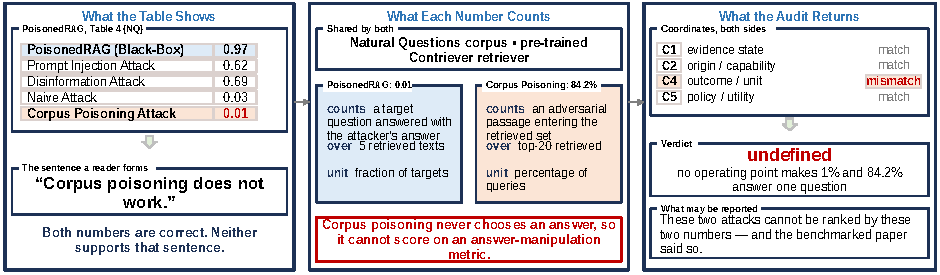
\includegraphics[width=0.90\textwidth]{figures/generated/fig_motivating_case.pdf}%
\caption{One case, in full. Two numbers that share a corpus and a retriever and
still cannot be ranked, because they count different events in different units
over different retrieved sets. Every value and every quoted condition is
re-opened at its cited line range by a released verifier
(\MotivPassed{}/\MotivChecks{} checks pass).}
\label{fig:motivating-case}
\end{figure*}


Both numbers are correct, and neither paper misreports anything. They share a corpus and a
Contriever retriever, but they differ in the size of the retrieved set (top-20 versus five
texts) and, decisively, in the event being counted. Corpus poisoning scores retrieval
success---``the percentage of queries for which at least one adversarial passage is retrieved
in the top-$k$ results'' \citep[l.~333--337]{poisoningRetrievalCorpora2023}---whereas
PoisonedRAG scores end-to-end generation success, that is, whether the model emits the
attacker's target string. PoisonedRAG says as much, noting that the weakest baselines ``are
ineffective because they cannot achieve generation, generation, and retrieval condition,
respectively'' [sic] \citep[l.~1338--1341]{poisonedRAG2024}; we reproduce the sentence as
printed and, together with six further checks behind Figure~\ref{fig:motivating-case}, verify
it against the source with a released tool (\MotivPassed{}/\MotivChecks{}). Inside
PoisonedRAG's own harness the $0.01$ is exactly right; carried across the harness boundary it
is a comparison between two different events. Cases like this are why we think a survey of
this field should say when two published numbers answer the same question, instead of ranking
them.

\paragraph{Contributions.}
\textbf{(i)} We survey robust RAG along four failure surfaces---evidence, model, adversary and
system control---organised around the contrasts between papers rather than around a list of
methods (\S\ref{sec:evidence}--\S\ref{sec:system}).
\textbf{(ii)} We reduce those surfaces to five \emph{reporting coordinates} and an explicit
three-way decision procedure that says when a quoted gap survives, narrows, or is undefined
(\S\ref{sec:coordinates}).
\textbf{(iii)} We then \emph{test the taxonomy as an instrument}: coordinates are recoverable
from prose that states them (\InsFullCoord{} accuracy, $\kappa$ \InsFullK{}), and we
characterise where recovery breaks down, including an arm on which a constant baseline beats
every model judge (\S\ref{sec:tested}).
\textbf{(iv)} We apply it at scale to \FrameCandidates{} candidate cross-paper comparisons
screened from \FlowTexts{} full texts, finding that \ProvReimplemented{} of \ProvClassified{}
classified pairs re-implement their baselines locally rather than transporting numbers, and
that adjudicating whether a gap survives stays underdetermined for automated panels and human
experts alike (\S\ref{sec:applied}).
\textbf{(v)} We derive reporting guidelines from those measurements rather than from
intuition (\S\ref{sec:practice}).

\paragraph{Relation to prior audits.}
Asking whether published numbers are comparable has precedent outside RAG.
\citet{marie2021credibility} hand-coded 769 machine translation papers and found comparisons
drawn across incomparable configurations to be routine, and \citet{bowman2021benchmarking},
\citet{gehrmann2023cracked} and \citet{howcroft2020twenty,vanderlee2021human,clark2021human}
document analogous problems in benchmarking and human evaluation. What is new here is the
combination: no RAG survey has tested whether its own categories are extractable from paper
text, and few audits report the point at which adjudication becomes underdetermined rather
than merely difficult. Since our pipeline leans on LLM judges, whose reliability is itself
contested \citep{zheng2023judging,panickssery2024selfpreference,wang2024fairevaluators}, we
treat evaluator reliability as a quantity to be measured---with human expert panels and
developer-independence checks---rather than as an assumption.

\section{Scope, Protocol and Evidence Base}
\label{sec:protocol}

\paragraph{Scope.}
We survey work in which a retrieval-augmented generator has to behave sensibly when the
evidence it receives is imperfect. The relevant conditions are irrelevant retrieval,
insufficient context, conflicts between sources or between a source and the model's own
parameters, stale or weakly attributed material, and deliberately corrupted passages. Two
neighbouring literatures fall outside this scope: retrieval studies that never generate an
answer, and generation studies that never retrieve. Neither exhibits the interaction we care
about, namely a generator committing to an answer on the basis of evidence it did not choose
and cannot fully trust.

\paragraph{Search and screening.}
We ran \FlowQueries{} arXiv queries together with five venue and repository sources at
snapshot \FlowSnapshot{}, returning \FlowRetrieved{} records. Of these, \FlowOpenPDF{} had
open PDFs, \FlowDedup{} survived deduplication, \FlowScreened{} passed relevance screening,
and \FlowTexts{} full texts were extracted and indexed into overlapping windows. The
screening rules and the scripts that apply them are released, and the PRISMA flow is
reproduced as Appendix Figure~\ref{fig:screening-frame-flow}. One stage is documented but not
re-executable: per-query hit counts were not logged at the snapshot date and live indices
drift, so everything from the \FlowTexts{} extracted texts downward can be re-run, while the
population those texts were drawn from cannot be reconstructed exactly. We therefore keep two
activities apart throughout. The narrative synthesis of
\S\ref{sec:evidence}--\S\ref{sec:system} draws on the broader literature and cites it
directly; every number we report is stated for the screening frame, never for the field.

\paragraph{Frame coverage and audit.}
Because a frame that missed most of the field would make even frame-local numbers hard to
read, we audited it against outside evidence. We took the bibliographies of \CovNSurveys{}
prior surveys (\S\ref{sec:coordinates}), title-screened them for robust-RAG scope, and
matched \CovPooledInScope{} unique references against our index. Recall is moderate rather
than high: \CovRecallTextsPct\% \CovRecallTextsCI{} of those references reach our
\FlowTexts{} full texts. The misses follow a systematic pattern---they name a specific system
architecture in the title without using any scope term---which is why
Sections~\ref{sec:evidence}--\ref{sec:system} cite the wider literature rather than the frame
alone (Appendix Table~\ref{tab:frame-coverage}). The narrative rests on a released
\MapRows{}-row evidence map recording, for each paper, the failure surface it addresses, the
intervention it makes, the benchmarks it uses, and the metrics it reports. Because that map
is preprint-heavy, we re-check every empirical claim on the peer-reviewed stratum alone
(\MapPeerReviewed{} rows; Appendix Table~\ref{tab:peer-reviewed-backbone}).


% Survey outline for Robust RAG. Top-down tree with live representative
% citations per leaf, using natbib aliases for compact rendering.

\definecolor{rragRootBd}{HTML}{2C3340}
\definecolor{rragLeafBg}{HTML}{F6F3EA}
\definecolor{rragLeafBd}{HTML}{C8C0B0}
\definecolor{rragBg}{HTML}{5B7393}  % background -- slate blue
\definecolor{rragEv}{HTML}{A06058}  % evidence -- muted brick
\definecolor{rragMd}{HTML}{5E8466}  % model -- forest sage
\definecolor{rragAt}{HTML}{8B6B91}  % adversarial -- plum
\definecolor{rragCt}{HTML}{4D8786}  % control -- teal
\definecolor{rragFu}{HTML}{A98552}  % future/guidelines -- ochre

% Compact aliases keep the outline readable while preserving live citations.
\defcitealias{lewis2020rag}{RAG}
\defcitealias{ragSurvey2024}{RAG-Survey}
\defcitealias{ragComprehensive2025}{RAG-Frontiers}
\defcitealias{ragEvaluationSurvey2024}{Eval-Survey}
\defcitealias{trustRAGCompass2024}{Trust-Compass}
\defcitealias{trustworthyRAGSurvey2025}{Trustworthy-RAG}
\defcitealias{securityRAGSurvey2026}{Secure-RAG}
\defcitealias{irrelevantContext2023}{IrrelCtx}
\defcitealias{raat2024}{RAAT}
\defcitealias{rgb2023}{RGB}
\defcitealias{ragTruth2024}{RAGTruth}
\defcitealias{queryRobustness2025}{QueryRobust}
\defcitealias{chainOfNote2023}{CoN}
\defcitealias{sufficientContext2024}{SuffCtx}
\defcitealias{tugOfWar2024}{Tug-of-War}
\defcitealias{faithfulRAG2025}{FaithfulRAG}
\defcitealias{astuteRAG2025}{AstuteRAG}
\defcitealias{poisoningRetrievalCorpora2023}{PoisonRetr}
\defcitealias{poisonedRAG2024}{PoisonedRAG}
\defcitealias{badRAG2024}{BadRAG}
\defcitealias{trojanRAG2024}{TrojanRAG}
\defcitealias{phantom2024}{Phantom}
\defcitealias{aip2025}{AIP}
\defcitealias{certifiedRAG2024}{RobustRAG}
\defcitealias{selfRAG2023}{Self-RAG}
\defcitealias{whenToRetrieve2024}{Adapt-LLM}
\defcitealias{ctrla2025}{CtrlA}
\defcitealias{crag2024}{CRAG}
\defcitealias{calibRAG2025}{CalibRAG}
\defcitealias{uncertaintyRAG2024}{UncertaintyRAG}
% --- rrag aliases ---
\defcitealias{rrag001}{URAG}
\defcitealias{rrag002}{SABER}
\defcitealias{rrag003}{FirstDrop}
\defcitealias{rrag004}{ProGRank}
\defcitealias{rrag005}{RetrBarrier}
\defcitealias{rrag006}{OverSearch}
\defcitealias{rrag007}{NAACL-Cal}
\defcitealias{rrag008}{CoRect}
\defcitealias{rrag009}{CleanBase}
\defcitealias{rrag010}{AdvCoT}
\defcitealias{rrag011}{SparseAtt-Def}
\defcitealias{rrag012}{UE-Axioms}
\defcitealias{rrag013}{TrustRAG}
\defcitealias{rrag014}{PoisonTrace}
\defcitealias{rrag015}{AVFilter}
\defcitealias{rrag016}{SecureRAG-Def}
\defcitealias{rrag017}{SeCon-RAG}
\defcitealias{rrag018}{GMTP}
\defcitealias{rrag019}{SafeRAG}
\defcitealias{rrag020}{Rescue-Unp}
\defcitealias{rrag021}{ReliabilityRAG}
\defcitealias{rrag023}{PoisonArena}
\defcitealias{rrag024}{ParamMute}
\defcitealias{rrag027}{MagicMushroom}
\defcitealias{rrag028}{MIRAGE}
\defcitealias{rrag029}{MAGIC}
\defcitealias{rrag030}{DontKnow}
\defcitealias{rrag031}{DRAGged}
\defcitealias{rrag032}{CUB}
\defcitealias{rrag033}{Poison-Bench}
\defcitealias{rrag034}{AdaRetr-Bench}
\defcitealias{rrag035}{LIAR}
\defcitealias{rrag036}{WikiContradict}
\defcitealias{rrag037}{RobustRALM}
\defcitealias{rrag038}{Trust-Or-Not}
\defcitealias{rrag039}{LC-RAG}
\defcitealias{rrag040}{FaithEval}
\defcitealias{rrag041}{Counterfactual}
\defcitealias{rrag042}{Context-DPO}
\defcitealias{rrag043}{Gullible}
\defcitealias{rrag044}{FILCO}
\defcitealias{rrag045}{KnowBoundary}
\defcitealias{rrag046}{Chameleon}
\defcitealias{rrag051}{GraphRAG-Fire}
\defcitealias{rrag055}{WorseZS}
\defcitealias{rrag058}{UDCG}
\defcitealias{rrag064}{UQ-Reason}
\defcitealias{rrag066}{Divide-Align}
\defcitealias{rrag073}{Denoise-First}
\defcitealias{rrag077}{ERA}
\defcitealias{rrag087}{Merlin-RAG}
\defcitealias{rrag088}{ProbeRAG}
\defcitealias{rrag092}{AfterRetr}
\defcitealias{rrag093}{SURE-RAG}
\defcitealias{rrag095}{BalanceRAG}
\defcitealias{rrag105}{FaithUQ}
\defcitealias{rrag107}{DeRAG}
\defcitealias{rrag111}{Unanswerability}
\defcitealias{rrag112}{RealConflict}
\defcitealias{rrag115}{RAFT}
\defcitealias{rrag127}{GraphPoison}
\defcitealias{rrag128}{Traceback}
\defcitealias{rrag131}{DistrAware}
\defcitealias{rrag132}{SourcePref}
\defcitealias{rrag134}{Secure-Survey}
\defcitealias{rrag136}{Curse-Help}
\defcitealias{rrag141}{MTRAG-UN}
\defcitealias{rrag143}{LostInEvi}
\defcitealias{rrag153}{Decide-Retr}
\defcitealias{rrag154}{SLM-Use}
\defcitealias{rrag174}{CARE-RAG}
\defcitealias{rrag175}{StylePoison}
\defcitealias{rrag180}{PrismRAG}
\defcitealias{rrag182}{PKV-Fusion}
\defcitealias{rrag183}{PRGB}
\defcitealias{rrag193}{CRUMQs}
\defcitealias{rrag200}{END-Drop}
\defcitealias{rrag201}{DynContext}
\defcitealias{rrag206}{DSSP-RAG}
\defcitealias{rrag214}{Parenting}
\defcitealias{rrag219}{RAGE-ICL}
\defcitealias{rrag226}{RECOMP}
\defcitealias{rrag229}{MM-RAG-Risk}

\begin{figure*}[!t]
\vspace*{-0.35cm}%
\setlength{\abovecaptionskip}{4pt}%
\centering
\makebox[\textwidth][c]{%
\hspace*{-0.30cm}%
\begin{tikzpicture}[
  x=1cm,y=1cm,
  root/.style={
    draw=rragRootBd, fill=white, text=rragRootBd,
    rounded corners=2pt, line width=0.7pt,
    font=\tiny\bfseries, align=center,
    inner xsep=5pt, inner ysep=4pt, text width=4.35cm
  },
  branch/.style={
    draw=#1, fill=#1, text=white,
    rounded corners=2pt, line width=0pt,
    font=\tiny\bfseries, align=center,
    inner xsep=3pt, inner ysep=3pt, text width=2.22cm
  },
  leaf/.style={
    draw=rragLeafBd, fill=rragLeafBg, text=black!84,
    rounded corners=1.5pt, line width=0.25pt,
    font=\fontsize{4.4}{4.75}\selectfont, align=left,
    inner xsep=1.9pt, inner ysep=1.4pt, text width=2.66cm
  },
  link/.style={-Latex, line width=0.4pt, color=black!42},
  twig/.style={line width=0.35pt, color=black!38, rounded corners=2pt}
]
\newcommand{\leafGap}{6pt}

\node[root] (root) at (0,0) {\textsc{Robust RAG}\\\textsc{under Unreliable Evidence}};

\node[branch=rragBg] (b1) at (-8.50,-1.12) {\S1--\S2\\Background \&\\Taxonomy};
\node[branch=rragEv] (b2) at (-5.10,-1.12) {\S3\\Evidence-Centric\\Robustness};
\node[branch=rragMd] (b3) at (-1.70,-1.12) {\S4\\Model-Centric\\Robustness};
\node[branch=rragAt] (b4) at (1.70,-1.12) {\S5\\Adversarial\\Corruption};
\node[branch=rragCt] (b5) at (5.10,-1.12) {\S6--\S7\\Control \&\\Evaluation};
\node[branch=rragFu] (b6) at (8.50,-1.12) {\S8--\S11\\Synthesis,\\Guidelines \&\\Future};

\coordinate (rootFork) at (0,-0.62);
\draw[twig] (root.south) -- (rootFork);
\draw[twig] (rootFork -| b1.north) -- (rootFork -| b6.north);
\foreach \b in {b1,b2,b3,b4,b5,b6} {
  \draw[link] (rootFork -| \b.north) -- (\b.north);
}

% =============== Background and taxonomy ===============
\node[leaf] (b1l1) at (-8.50,-2.55) {\textbf{\S1~Problem framing}\\RAG as evidence-conditioned policy; running example\\{\color{black!62}\citetalias{lewis2020rag}, \citetalias{ragSurvey2024}, \citetalias{ragComprehensive2025}, \citetalias{trustRAGCompass2024}, \citetalias{trustworthyRAGSurvey2025}, \citetalias{rrag037}, \citetalias{queryRobustness2025}, \citetalias{rgb2023}}};
\node[leaf] (b1l2) at (-8.50,-4.20) {\textbf{Evidence reliability}\\relevance, sufficiency, faithfulness, consistency, integrity\\{\color{black!62}\citetalias{irrelevantContext2023}, \citetalias{sufficientContext2024}, \citetalias{tugOfWar2024}, \citetalias{faithfulRAG2025}, \citetalias{poisonedRAG2024}, \citetalias{badRAG2024}, \citetalias{rrag003}, \citetalias{rrag045}}};
\node[leaf] (b1l3) at (-8.50,-5.85) {\textbf{\S2~Comparability tuple}\\evidence-, model-, system-centric, evaluation layers\\{\color{black!62}\citetalias{trustRAGCompass2024}, \citetalias{trustworthyRAGSurvey2025}, \citetalias{ragComprehensive2025}, \citetalias{ragEvaluationSurvey2024}, \citetalias{securityRAGSurvey2026}, \citetalias{rrag073}, \citetalias{rrag134}, \citetalias{ragSurvey2024}}};
\node[leaf] (b1l4) at (-8.50,-7.50) {\textbf{Operational pipeline}\\detect, diagnose, mitigate, control, monitor\\{\color{black!62}\citetalias{chainOfNote2023}, \citetalias{crag2024}, \citetalias{sufficientContext2024}, \citetalias{selfRAG2023}, \citetalias{ctrla2025}, \citetalias{calibRAG2025}, \citetalias{rrag002}, \citetalias{astuteRAG2025}}};

% =============== Evidence-centric (Section 4) ===============
\node[leaf] (b2l1) at (-5.10,-2.55) {\textbf{Noisy retrieval}\\irrelevant passages, hard negatives, missing positives\\{\color{black!62}\citetalias{irrelevantContext2023}, \citetalias{raat2024}, \citetalias{rgb2023}, \citetalias{rrag027}, \citetalias{rrag001}, \citetalias{rrag037}, \citetalias{rrag043}, \citetalias{rrag055}, \citetalias{rrag030}}};
\node[leaf] (b2l2) at (-5.10,-4.20) {\textbf{Distraction}\\negative context utility, ordering, long-context erosion\\{\color{black!62}\citetalias{rrag003}, \citetalias{rrag032}, \citetalias{rrag039}, \citetalias{rrag058}, \citetalias{rrag131}, \citetalias{rrag136}, \citetalias{rrag143}, \citetalias{rrag180}, \citetalias{rrag200}, \citetalias{rrag201}}};
\node[leaf] (b2l3) at (-5.10,-5.85) {\textbf{Query- \& index-side noise}\\query perturbation, chunking, hybrid retrieval, multimodality\\{\color{black!62}\citetalias{queryRobustness2025}, \citetalias{rrag073}, \citetalias{rrag141}, \citetalias{rrag051}, \citetalias{rrag127}, \citetalias{rrag175}, \citetalias{rrag229}, \citetalias{rrag182}}};
\node[leaf] (b2l4) at (-5.10,-7.50) {\textbf{Evidence-side controls}\\filtering, reranking, compression, query repair\\{\color{black!62}\citetalias{rrag044}, \citetalias{rrag226}, \citetalias{rrag092}, \citetalias{rrag004}, \citetalias{rrag017}, \citetalias{rrag154}, \citetalias{rrag020}, \citetalias{rrag073}}};

% =============== Model-centric (Section 5) ===============
\node[leaf] (b3l1) at (-1.70,-2.55) {\textbf{Context utilization}\\notes, filtering, claim-level support, intermediate reasoning\\{\color{black!62}\citetalias{chainOfNote2023}, \citetalias{rrag032}, \citetalias{rrag115}, \citetalias{rrag226}, \citetalias{rrag088}, \citetalias{rrag042}, \citetalias{rrag038}, \citetalias{rrag040}}};
\node[leaf] (b3l2) at (-1.70,-4.20) {\textbf{Knowledge conflict}\\parametric vs.\ retrieved, retrieved vs.\ retrieved, sources\\{\color{black!62}\citetalias{tugOfWar2024}, \citetalias{faithfulRAG2025}, \citetalias{astuteRAG2025}, \citetalias{rrag008}, \citetalias{rrag024}, \citetalias{rrag029}, \citetalias{rrag031}, \citetalias{rrag036}, \citetalias{rrag112}, \citetalias{rrag174}}};
\node[leaf] (b3l3) at (-1.70,-5.85) {\textbf{Faithful generation \& attribution}\\citations, verification, source reliability, hallucination\\{\color{black!62}\citetalias{ragTruth2024}, \citetalias{rrag206}, \citetalias{rrag132}, \citetalias{rrag115}, \citetalias{rrag017}, \citetalias{rrag013}, \citetalias{rrag045}, \citetalias{rrag046}, \citetalias{rrag092}}};
\node[leaf] (b3l4) at (-1.70,-7.50) {\textbf{Limits of model-centric fixes}\\suppression vs.\ trust, situated faithfulness, robust training\\{\color{black!62}\citetalias{rrag024}, \citetalias{rrag038}, \citetalias{rrag042}, \citetalias{rrag043}, \citetalias{rrag214}, \citetalias{rrag112}, \citetalias{rrag066}, \citetalias{rrag077}}};

% =============== Adversarial corruption (Section 6) ===============
\node[leaf] (b4l1) at (1.70,-2.55) {\textbf{Corpus poisoning \& backdoors}\\malicious passages, triggers, knowledge corruption\\{\color{black!62}\citetalias{poisoningRetrievalCorpora2023}, \citetalias{poisonedRAG2024}, \citetalias{badRAG2024}, \citetalias{trojanRAG2024}, \citetalias{phantom2024}, \citetalias{rrag010}, \citetalias{rrag028}, \citetalias{rrag035}, \citetalias{rrag175}, \citetalias{rrag127}}};
\node[leaf] (b4l2) at (1.70,-4.20) {\textbf{Prompt-level \& injection attacks}\\indirect injection, template attacks, agent attacks\\{\color{black!62}\citetalias{aip2025}, \citetalias{rrag005}, \citetalias{rrag107}, \citetalias{rrag019}, \citetalias{rrag051}, \citetalias{rrag023}, \citetalias{rrag033}, \citetalias{rrag214}}};
\node[leaf] (b4l3) at (1.70,-5.85) {\textbf{Defense-in-depth}\\sanitization, robust retrieval, attention filters, traceback\\{\color{black!62}\citetalias{certifiedRAG2024}, \citetalias{rrag004}, \citetalias{rrag009}, \citetalias{rrag011}, \citetalias{rrag013}, \citetalias{rrag014}, \citetalias{rrag015}, \citetalias{rrag016}, \citetalias{rrag018}, \citetalias{rrag020}, \citetalias{rrag021}, \citetalias{rrag128}}};
\node[leaf] (b4l4) at (1.70,-7.50) {\textbf{Threat models \& attack realism}\\attacker knowledge, retrieval realism, stealth, benchmarks\\{\color{black!62}\citetalias{rrag005}, \citetalias{rrag019}, \citetalias{rrag023}, \citetalias{rrag033}, \citetalias{rrag028}, \citetalias{rrag015}, \citetalias{securityRAGSurvey2026}, \citetalias{rrag134}}};

% =============== Control and evaluation (Sections 7-8) ===============
\node[leaf] (b5l1) at (5.10,-2.55) {\textbf{Adaptive retrieval}\\when to retrieve, re-retrieve, stop, decompose\\{\color{black!62}\citetalias{selfRAG2023}, \citetalias{whenToRetrieve2024}, \citetalias{ctrla2025}, \citetalias{crag2024}, \citetalias{rrag006}, \citetalias{rrag034}, \citetalias{rrag153}, \citetalias{rrag066}, \citetalias{rrag077}}};
\node[leaf] (b5l2) at (5.10,-4.20) {\textbf{Calibration, abstention \& uncertainty}\\confidence, refusal, clarification, conformal control\\{\color{black!62}\citetalias{calibRAG2025}, \citetalias{uncertaintyRAG2024}, \citetalias{rrag002}, \citetalias{rrag007}, \citetalias{rrag012}, \citetalias{rrag041}, \citetalias{rrag064}, \citetalias{rrag087}, \citetalias{rrag095}, \citetalias{rrag105}, \citetalias{rrag111}, \citetalias{rrag141}, \citetalias{rrag193}}};
\node[leaf] (b5l3) at (5.10,-5.85) {\textbf{Policy composition \& cost-aware control}\\over-retrieval, cost--latency budgets, escalation, interaction\\{\color{black!62}\citetalias{rrag006}, \citetalias{rrag034}, \citetalias{rrag111}, \citetalias{rrag141}, \citetalias{rrag041}, \citetalias{rrag002}, \citetalias{rrag066}, \citetalias{rrag038}}};
\node[leaf] (b5l4) at (5.10,-7.50) {\textbf{Evaluation \& benchmarks}\\noise, conflict, attacks, selective risk, action quality\\{\color{black!62}\citetalias{rgb2023}, \citetalias{ragTruth2024}, \citetalias{queryRobustness2025}, \citetalias{rrag001}, \citetalias{rrag019}, \citetalias{rrag023}, \citetalias{rrag027}, \citetalias{rrag029}, \citetalias{rrag036}, \citetalias{rrag040}, \citetalias{rrag093}, \citetalias{rrag183}}};

% =============== Synthesis / guidelines / future (Sections 9-12) ===============
\node[leaf] (b6l1) at (8.50,-2.55) {\textbf{Design principles}\\evidence as constructed context, source reliability, action quality\\{\color{black!62}\citetalias{rrag058}, \citetalias{rrag132}, \citetalias{rrag111}, \citetalias{sufficientContext2024}, \citetalias{astuteRAG2025}, \citetalias{chainOfNote2023}, \citetalias{calibRAG2025}, \citetalias{rrag038}}};
\node[leaf] (b6l2) at (8.50,-4.20) {\textbf{Cross-cutting analysis}\\intervention points, method families, Pareto progress\\{\color{black!62}\citetalias{irrelevantContext2023}, \citetalias{chainOfNote2023}, \citetalias{sufficientContext2024}, \citetalias{certifiedRAG2024}, \citetalias{rrag004}, \citetalias{rrag013}, \citetalias{astuteRAG2025}, \citetalias{ragComprehensive2025}}};
\node[leaf] (b6l3) at (8.50,-5.85) {\textbf{Practical guidelines}\\for benchmark builders, method designers, system builders\\{\color{black!62}\citetalias{rrag019}, \citetalias{rrag023}, \citetalias{rrag027}, \citetalias{rrag033}, \citetalias{rrag034}, \citetalias{rrag141}, \citetalias{rrag193}, \citetalias{certifiedRAG2024}, \citetalias{rrag013}, \citetalias{rrag017}}};
\node[leaf] (b6l4) at (8.50,-7.50) {\textbf{Open challenges \& future}\\joint benchmarks, agentic/multimodal RAG, versioned maps\\{\color{black!62}\citetalias{rrag051}, \citetalias{rrag127}, \citetalias{rrag175}, \citetalias{rrag229}, \citetalias{rrag219}, \citetalias{trustworthyRAGSurvey2025}, \citetalias{securityRAGSurvey2026}, \citetalias{rrag134}}};

\foreach \b/\last in {b1/b1l4,b2/b2l4,b3/b3l4,b4/b4l4,b5/b5l4,b6/b6l4} {
  \coordinate (\b fork) at ($(\b.south)+(0,-0.18)$);
  \draw[twig] (\b.south) -- (\b fork) -| ([xshift=\leafGap]\last.east);
}
\foreach \l in {b1l1,b1l2,b1l3,b1l4,b2l1,b2l2,b2l3,b2l4,b3l1,b3l2,b3l3,b3l4,b4l1,b4l2,b4l3,b4l4,b5l1,b5l2,b5l3,b5l4,b6l1,b6l2,b6l3,b6l4} {
  \draw[link] ([xshift=\leafGap]\l.east) -- (\l.east);
}

\end{tikzpicture}%
}
\caption{\textbf{Outline of this paper.} A top-down view of the paper structure. The root problem is robust RAG under unreliable evidence; the paper then moves from background and taxonomy to evidence-centric, model-centric, adversarial, system-control, evaluation, synthesis, and future-facing guidelines. Each leaf lists representative cited work using compact aliases.}
\label{fig:survey_outline}
\end{figure*}


\section{The Four Failure Surfaces}
\label{sec:taxonomy}

A RAG system is best read as an evidence-conditioned decision process: a query arrives, a
retriever assembles a context, and a generator commits to an action on the basis of that
context. Failures occur when the assembled evidence is incomplete, irrelevant, misleading,
mutually contradictory, corrupted, or simply insufficient to support any answer
(Appendix~\ref{app:background}). Sorting the literature by \emph{where} in this process a
paper intervenes yields four failure surfaces, which we use as the top-level organisation of
the survey and summarise in Figure~\ref{fig:survey_outline}.

\textbf{Evidence-centric} work (\S\ref{sec:evidence}) treats the composition of the context
as the object of study, asking which passages reach the generator and in what order.
\textbf{Model-centric} work (\S\ref{sec:model}) holds the context fixed and asks how the
generator uses it, which is where faithfulness, attribution and knowledge conflict live.
\textbf{Adversarial} work (\S\ref{sec:adversarial}) replaces the assumption of benign noise
with an adaptive attacker who chooses the evidence. \textbf{System-centric} work
(\S\ref{sec:system}) steps outside the single forward pass and asks what the system should
\emph{do}---retrieve again, verify, abstain, or answer---under uncertainty and cost.

The four surfaces partition the literature, not the phenomena, and a single event routinely
touches several at once. A poisoned passage is an evidence state, an adversary capability,
and---if the system declines to answer because of it---a policy decision. That overlap is
exactly why placing two papers on the same surface does not make their numbers comparable,
and it motivates the reduction to five reporting coordinates in \S\ref{sec:coordinates}.
Evaluation practice cuts across all four surfaces and is treated separately in
Appendix~\ref{app:evaluation}; the rules used to assign a paper to a surface are in
Appendix~\ref{sec:appendix-methods}.


\section{Evidence-Centric Robustness}
\label{sec:evidence}

Evidence-centric work takes the context window itself as the object of study: what the
retriever puts in front of the generator, in what order, and at what budget
(Appendix~\ref{app:evidence}). The stakes are higher here than in classical retrieval,
because the retrieved set is not a ranked list a user inspects but a prompt a model reads,
and a single misleading passage can move the answer, the stated confidence, and the citations
all at once.

\paragraph{Noise is not one condition.}
The most consequential distinction in this literature is between failing to fetch the right
evidence and failing to ignore the wrong evidence. \citet{irrelevantContext2023} separate the
two explicitly, and \citet{raat2024} show that the second is far harder than it looks: clearly
off-topic passages are discarded easily, whereas semantically close counterfactuals and hard
negatives are not. RGB makes the same point by construction, scoring noise robustness,
negative rejection and counterfactual handling as three separate abilities rather than one
\citep{rgb2023}. The practical consequence is that a single robustness-under-noise number is
uninterpretable on its own, because two papers reporting it may be stressing different
abilities.

\paragraph{Context construction has negative marginal utility.}
Adding passages is not monotone. \citet{cuconasu2024powerofnoise} find that topically related
but wrong passages hurt generation while purely random text can occasionally stabilise it, and
\citet{liu2024lostmiddle} show that the same passage helps or hurts depending on where it sits
in the prompt. Longer contexts do not resolve this: hard negatives and misleading content
continue to degrade reasoning as the window grows \citep{rrag039,rrag003}. Benchmarks such as
CUB \citep{rrag032} and UDCG \citep{rrag058} follow this observation to its conclusion and score
retrieval by downstream utility rather than by relevance, treating the retriever as an active
constructor of the model's input rather than as a passive supplier of documents.

\paragraph{Mitigations trade one failure for another.}
Evidence-side defences---filtering \citep{rrag044}, compression and reordering \citep{rrag039},
utility-aware reranking \citep{rrag058}, and noise-aware training \citep{raat2024}---all buy
precision with recall, so a defence that improves accuracy under distraction may lose answers
that a noisier pipeline would have found. Interventions on the query and index side, such as
rephrasing \citep{queryRobustness2025} or chunking and graph construction
\citep{rrag141,rrag051}, add failure surfaces of their own. None of these results transfers
across papers unless the corpus snapshot, retriever, and top-$k$ are stated, which is the
content of coordinate C1 in \S\ref{sec:coordinates}.


\section{Model-Centric Robustness}
\label{sec:model}

Model-centric work holds the retrieved set fixed and asks what the generator does with it
(Appendix~\ref{app:model}). Given identical context, models differ in how closely they follow
instructions, how strongly they defer to their parametric priors, how much of the prompt they
actually consult, and how well their stated confidence tracks correctness.

\paragraph{Availability is not utilisation.}
A passage being present in the prompt does not mean it was used, and an unsupported passage may
drive the answer more than the gold one. Chain-of-Note makes this explicit by summarising each
passage, judging its relevance, and abstaining when the set is insufficient
\citep{chainOfNote2023}, while benchmarks such as CUB score whether a model leans on gold
evidence while ignoring plausible distractors \citep{rrag032}. Reporting only end-task accuracy
collapses the two, so a system that answers correctly for the wrong reason is scored as robust.

\paragraph{Knowledge conflict is structural, not incidental.}
Retrieval augmentation puts a model's memory, its retrieved context, and multiple retrieved
sources in the same prompt, and these can disagree. \citet{longpre2021conflicts} formalised the
first case through entity substitution, and \citet{xie2024chameleon} showed that models comply
with coherent counter-evidence but resist incoherent claims, favouring what they already
believe. Two opposite failures follow---over-compliance with false retrieved content and
over-reliance on stale memory---and a study that fixes one can worsen the other
\citep{tugOfWar2024}. Mitigations differ in where they act: localising the disagreement
\citep{faithfulRAG2025}, editing activations \citep{rrag008}, or aggregating evidence weighted by
source reliability \citep{astuteRAG2025}. Because \emph{resolving conflict} can mean answering
correctly, following the context, or reconciling sources, papers that share the label often
optimise different objectives.

\paragraph{Citing is not grounding.}
Source-preference frameworks ask which evidence wins under conflict \citep{rrag132,rrag110}, and
a recurring finding is that a produced citation is weak proof of support: models cite passages
that are topically aligned but do not entail the claim \citep{ragTruth2024}. Reference-free
evaluation suites accordingly separate faithfulness, relevance, and precision instead of merging
them \citep{ragas2024,ares2024}. Since all of these quantities are defined relative to the
evidence the model saw, comparing two generators is only meaningful when the evidence state is
held constant on both sides.


\section{Adversarial Corruption and Security}
\label{sec:adversarial}

Adversarial work removes the assumption that unreliable evidence arrives by accident and
replaces it with an attacker who chooses the evidence (Appendix~\ref{app:adversarial}).
Because RAG externalises knowledge into corpora, indices, prompt templates and tools, every
one of these becomes an attack surface that a purely parametric model does not have.

\paragraph{Poisoning turns small corpus edits into large output changes.}
\citet{poisoningRetrievalCorpora2023} showed that a handful of crafted passages is enough to
distort a dense retriever's neighbourhood structure, and PoisonedRAG carried the same idea
through to the generated answer \citep{poisonedRAG2024}. Later work varies the trigger and the
persistence model: BadRAG studies triggered retrieval \citep{badRAG2024}, while TrojanRAG and
Phantom induce attacker-chosen behaviour through retrieved context alone, without touching
model weights \citep{trojanRAG2024,phantom2024}. What these share is an amplification effect:
retrieval converts a marginal perturbation of the corpus into a first-class input to the model.

\paragraph{Injection and poisoning are different threats.}
Indirect prompt injection plants \emph{executable instructions} rather than false evidence, and
the payload must first clear a retrieval barrier before it can act \citep{rrag005}; AIP instead
exploits prompts shared across users \citep{aip2025}. The distinction matters for defence
design, because a filter tuned to detect implausible claims will not detect a plausible
document that ends with an instruction. Treating templates, ingestion pipelines and retrieved
text as untrusted boundaries is therefore a stronger design stance than treating the corpus as
the only thing to sanitise.

\paragraph{Defences are not comparable across threat models.}
Proposed defences span certified aggregation \citep{certifiedRAG2024}, adversarial reranking
\citep{rrag004}, attention-level filtering \citep{rrag015}, and post-hoc traceback of the
responsible passage \citep{rrag128}, and each is evaluated against the threat its authors
assumed. Two further sources of divergence are less visible. Papers differ in what the
attacker is allowed to know and do, and they differ in the unit that the attack budget is
counted in---documents injected into the corpus versus documents actually retrieved into the
context---so nominally identical budgets can differ by an order of magnitude. Reporting
adversary access and budget scope, coordinate C2 in \S\ref{sec:coordinates}, is what makes two
attack success rates commensurable. Recent evaluation suites move this way, fixing
corpus, retriever and injection budget before pitting attacks against one another
\citep{rrag019,rrag023,rrag033}.


\section{System-Centric Control}
\label{sec:system}

System-centric work treats RAG as a policy rather than a fixed pipeline
(Appendix~\ref{app:system}). The system decides whether to retrieve at all, how much context
to admit, whether to verify, when to fall back on parametric memory, and---most consequentially---whether
to answer or decline.

\paragraph{Sufficiency and confidence answer different questions.}
The negative-rejection condition in RGB shows that systems routinely answer when the evidence
does not license an answer \citep{rgb2023}, and Sufficient Context reframes evaluation around
whether the retrieved set can support an answer at all \citep{sufficientContext2024}, a framing
that unanswerability benchmarks extend to multi-turn and open-domain settings
\citep{rrag111,rrag141}. Keeping the two apart is essential: \emph{evidence uncertainty} asks
whether the context supports the query, \emph{model uncertainty} asks whether the generator can
use it correctly. High confidence under low sufficiency is hallucination on top of false
context, whereas low confidence under adequate evidence calls for verification, not refusal.

\paragraph{The action space is wider than answer-or-abstain.}
Self-RAG, adaptive-retrieval classifiers, CtrlA and Corrective RAG all gate retrieval, using
reflection tokens, learned predictors, internal confidence signals, or evidence-quality
thresholds respectively \citep{selfRAG2023,whenToRetrieve2024,ctrla2025,crag2024}; because each
buys accuracy with calls, they are only comparable on an accuracy--cost plane rather than at a
single point \citep{rrag006}. Beyond gating, a deployed system can ask a clarifying question,
re-retrieve, or surface the contradiction instead of resolving it \citep{rrag141}. This is why
a reported ``abstention rate'' is not yet a result: without the action set and the loss attached
to each action---coordinate C5 in \S\ref{sec:coordinates}---the same number can describe a
cautious system and a useless one. The difficulty is empirical rather than hypothetical: C5 is
not extractable at all from \SilentPct{}\% of the text windows in our census.

\paragraph{Beyond one modality and one turn.}
These questions return in harder form once retrieval spans modalities, tools, or several
interacting agents, where one unreliable passage can be reused across turns and propagated
between sub-agents \citep{rrag229,rrag219,rrag051}. That literature is still thin, and it
inherits every reporting problem above: the action set grows, error costs become
path-dependent, and the unit of measurement stops being a single question.


\section{From Four Surfaces to Five Reporting Coordinates}
\label{sec:coordinates}
\label{sec:estimands}

The four surfaces tell a reader where a paper sits, but they do not tell a reader whether two
papers' numbers may be placed side by side. For that we need a description of each \emph{side}
of a comparison rather than of each paper. We use five reporting coordinates, each one a
compression of a question the surfaces above already raise.

\begin{itemize}[leftmargin=1.15em,itemsep=1.5pt,topsep=2.5pt,parsep=0pt]
\item[\textbf{C1}] \emph{Evidence state} (\S\ref{sec:evidence}): what the context looks like at
the decision point---supported, distracting, insufficient, conflicting, stale, weakly sourced,
or manipulated---together with the corpus snapshot, retriever, top-$k$, and whether a gold
passage is present at all.
\item[\textbf{C2}] \emph{Origin and capability} (\S\ref{sec:adversarial}): how that state came
about, whether through benign retrieval error, a synthetic stressor, distribution drift, or an
adaptive adversary; for attacks, the adversary's access, persistence, budget unit (documents
injected versus documents retrieved), and whether the score is over all queries or only
triggered ones.
\item[\textbf{C3}] \emph{Intervention} (\S\ref{sec:model}): where the change is made, from the
corpus and retriever through the generator to a verifier module or the evaluation artifact.
\item[\textbf{C4}] \emph{Outcome and unit}: what is scored---answer correctness, retrieval
quality, claim support, attack success, leakage, calibration error, or cost---and per what
unit: a question, a response, or a span.
\item[\textbf{C5}] \emph{Policy and utility} (\S\ref{sec:system}): the recourse available under
uncertainty---answer, verify, re-retrieve, expose the conflict, quarantine, or abstain---and the
costs attached to being wrong, refusing, and following up.
\end{itemize}

\paragraph{A decision procedure for a quoted gap.}
Once both sides are recorded, a gap between them is adjudicated in three steps.
\textbf{(1)}~If C1, C2, C4 and C5 match, the gap \emph{survives} and may be reported as stated.
\textbf{(2)}~If they do not match but one paper reports an operating point matching the other's
configuration, the comparison \emph{narrows} to that point and must be restated there.
\textbf{(3)}~Otherwise the gap is \emph{undefined}: the claim must be confined to the common
subset or withdrawn, not computed across the mismatch. The third outcome is the one current
practice lacks a vocabulary for, and \S\ref{sec:applied} shows how often it is the correct one.

\paragraph{Why C3 is recorded but not gated.}
The intervention coordinate is deliberately excluded from the rule above, and the reason is
definitional rather than empirical: two systems being compared differ in their intervention by
construction, so requiring C3 to match would declare every cross-system comparison invalid.
We nonetheless record C3 and report in \S\ref{sec:tested} exactly what this choice costs.

\paragraph{Relation to existing survey taxonomies.}
Prior surveys organise robust RAG by mechanism---noise types \citep{ragSurvey2024}, trust
dimensions \citep{trustRAGCompass2024}, attack vectors \citep{securityRAGSurvey2026}, conflict
types \citep{xuKnowledgeConflicts2024}, or abstention strategies \citep{wenAbstentionSurvey2025}---and
those structures are effective for finding related work. None of them structures the act of
comparison, and none tests whether paper text carries enough detail for its own categories to be
recovered. Comparability audits of this kind exist outside RAG, in translation, benchmarking and
human evaluation \citep{marie2021credibility,howcroft2020twenty,gehrmann2023cracked}, and our
coordinates adapt long-standing ideas from evidence synthesis, selective prediction and security
evaluation \citep{richardson1995pico,chow1970reject,papernot2018sok} to this setting (Appendix
Table~\ref{tab:main-prior-work-comparison}).


\section{Testing the Taxonomy}
\label{sec:tested}
\label{sec:instrument}

A taxonomy that cannot be applied by anyone other than its authors is a description of the
authors' intuitions. We therefore treat the coordinates of \S\ref{sec:coordinates} as an
instrument and measure it: can independent coders recover the coordinates from prose, what does
excluding C3 actually cost, and are five coordinates doing work that two would not? The coders
in this section are LLM judges from several providers; \S\ref{sec:applied} adds a human expert
panel.\footnote{Throughout, $\kappa$ is Fleiss' $\kappa$ over the panel, $\kappa_{\max}$ the
largest value attainable given the raters' marginals \citep{umesh1989maxkappa,sim2005kappa},
$AC_1$ is Gwet's prevalence-robust statistic, and ``observed'' is raw pairwise agreement. Under
skewed labels $\kappa$ is deflated by construction, so we report all four. Intervals are
percentile bootstrap over the stated cluster unit.}

\paragraph{Coordinates are recoverable when they are stated.}
We wrote \InsTwoItems{} short passages in the style of an experimental-setup paragraph, each
generated from a ground-truth specification of whether two settings agree on C1, C2, C4 and C5
and of which of them the text actually discloses; the correct verdict then follows
deterministically from the rule in \S\ref{sec:coordinates}. Disclosure varies across three
regimes---everything stated; something withheld but the verdict still fixed by what remains
(baseline \InsBalBase{}); and something withheld so that the correct answer is
\emph{underspecified} (a degenerate arm, baseline \InsForceBase{})---crossed with a
checklist-versus-prose presentation factor (Appendix~\ref{sec:appendix-instrument}). On the
\InsFullN{} fully disclosing passages, \InsTwoJudges{} judges recover coordinate labels with
\InsFullCoord{} accuracy and agree on the verdict at $\kappa$ \InsFullK{}. Over all
\InsTwoScored{} items the composed rule reaches \InsTwoRule{} against a constant baseline of
\InsTwoBase{}, and writing the same content as natural prose rather than as a checklist costs
almost nothing (\InsCanonCoord{} to \InsNatCoord{}). The instrument is therefore sound; what
follows is about the text it is applied to.

\paragraph{What excluding C3 costs.}
Since dropping C3 is a definitional choice, we report its consequences rather than defend it.
Across \CensusEligible{} eligible windows, majority vote marks C3 a mismatch on
\CthreeMismatchCount{} instances (\CThreeMismatchMaj\% of majority-classified items). Gating on
C3 would flip \CthreeGateChanged{} of \CthreeGateN{} composite verdicts and cut surviving
comparisons from \CthreeSurvWithout{} to \CthreeSurvWith{}, which is to say it would abolish
cross-paper comparison rather than discipline it. One statistic needs care here: inter-judge
$\kappa$ on C3 is near zero, but \PrevCThree\% of its labels fall in a single class, and under
that skew $\kappa$ is uninformative. Raw agreement is \ObsCThree{}, Gwet's $AC_1$ is $0.72$, and
$\kappa_{\max}$ is only \KmaxCThree{}: this is the prevalence paradox \citep{sim2005kappa}, not
an inability to read intervention descriptions.

\paragraph{Five coordinates versus two.}
On non-degenerate items the five-coordinate rule reaches \InsFiveAcc{} against \InsBestTwoAcc{}
for the best two-coordinate estimator (paired difference \InsFiveVsTwoDiff{}, exact McNemar
$p=\InsFiveVsTwoP$). On the degenerate arm ($N=\InsForceN$) five coordinates give \InsForceFive{}
and two give \InsForceTwo{}, yet both lose to a constant predictor that always answers
``underspecified'' (\InsForceBase{} by construction)---the clearest single sign that the
bottleneck is the source text rather than the schema. On real corpus data a reduced C1/C4
codebook performs comparably (\AblCFourDelta{} difference, \AblCFourCI{}). We read this as C1 and
C4 being the minimal pair a comparison cannot do without, while C2 and C5 earn their place by
naming the ambiguity that remains.


\section{The Taxonomy Applied at Scale}
\label{sec:applied}
\label{sec:census}

We now run the same instrument over published text. A deterministic screen across
\FlowTexts{} full texts isolates \FrameCandidates{} passages in which one paper's number is
placed beside another's, drawn from \FrameFiles{} papers
(Appendix~\ref{sec:appendix-census}); majority vote over three model judges keeps
\CensusEligible{} of them as genuine cross-paper comparisons ($\kappa$ \DecEligK{}). A second
pass asks a structural question about each survivor---were the compared baselines
\emph{transported} from their original papers, or \emph{re-implemented} locally?---and a third
asks the substantive one: does the quoted gap survive?

\paragraph{Most comparisons are made inside one harness.}
Of the \ProvClassified{} eligible candidates whose provenance could be classified,
\ProvReimplemented{} re-implement their baselines inside a single corpus, retriever, generator
and metric harness, and only \ProvTransported{} carry numbers across a harness boundary
(\ProvReimplPct{}\% re-implemented; \GateUnanSharePct{}\% under unanimous gating,
\GateLooRangePct{}\% across leave-one-out sensitivity). This is a reassuring finding about the
field, and it is one automation can be trusted with: judges agree at $\kappa$ \DecProvK{} and
reach \DepPvAcc{} \DepPvCI{} accuracy against reference adjudicators who read the full papers
(\DepPvN{} windows, baseline \DepPvBase{}; Appendix Table~\ref{tab:privileged-reference}).

\paragraph{Whether a gap survives is not decidable from the text.}
The substantive question behaves entirely differently. Over the same \CensusEligible{} windows,
verdict agreement is $\kappa$ \DecVerdictK{}---\KShareVerdict{}\% of the attainable ceiling
\KmaxVerdict{}, at observed agreement \ObsVerdict{}---and accuracy against reference
adjudicators is \DepVdAcc{} \DepVdCI{} over \DepVdN{} quote-verified windows (baseline
\DepVdBase{}). Bounding the \RefVdNoMaj{} windows with no majority gives worst and best cases of
\BoundVdCommitWorst{} and \BoundVdCommitBest{}. The failures are not subtle: the weakest judge
contradicts its own coordinate assignments on \RuleContraWorst{} of \RuleContraWorstN{} items
(rule fidelity \RuleFidelityLo{} versus \RuleFidelityHi{} for the strongest), and \QFAbsent{} of
\QFNonEmpty{} quoted pieces of evidence (\QFAbsentPct{}\%) cannot be found in the cited source.

\paragraph{The bottleneck is the prose, not the evaluator.}
To locate the cause we varied one thing at a time with the codebook and items fixed
(Figure~\ref{fig:interventions}). Supplying the whole paper instead of a window raises agreement
by \LadVdDeltaCite{} \LadVdDeltaCiteCI{}, confirming that windowing truncates relevant context
but not closing the gap. The remaining interventions barely move it: offering an explicit
\emph{underspecified} option shifts agreement by \AbsKDiff{} \AbsKDiffCI{}, composing the rule
deterministically by \RuleKDiff{} \RuleKDiffCI{}, \OwjNOpen{} open-weight models reach $\kappa$
\OwjKOpen{} ($\kappa_{\max}=\text{\OwjKmaxOpen{}}$), and a non-generative structural classifier
trained on reference verdicts reaches \NllVdStructAcc{} against a \NllVdBaseAcc{} baseline
(\NllVdStructdAcc{} \NllVdStructdAccCI{}).

Finally, we asked whether trained people do better. Three NLP and RAG researchers annotated
\HumN{} published claims over \HumHours{} person-hours with senior adjudication, reaching
$\kappa$ \HumVerdictK{} \HumVerdictKCI{} against a ceiling of \HumVerdictKmax{}; the model panel
scored $\kappa$ \HumModVerdictK{} on the same items, a difference of \HumGapDelta{}
\HumGapCI{}. A power analysis over \HumClusters{} clusters bounds any human advantage below
\HumMDE{}, and the experts spread as widely as the models in how many claims they were willing
to call valid (\HumSpreadLo{}\%--\HumSpreadHi{}\% versus \HumModSpreadLo{}\%--\HumModSpreadHi{}\%
across \HumModJudges{} models). Underdetermination therefore lives in what published papers say,
not in who is reading them.


\section{What Follows for Practice}
\label{sec:practice}

Three recommendations follow directly from the measurements above; extended versions are in
Appendices~\ref{app:guidelines} and~\ref{app:challenges}, and a one-page form is the checklist in
Appendix~\ref{sec:appendix-eval}.

\paragraph{State all five coordinates, and state C1 and C4 first.}
Evidence state and outcome unit are the pair that no comparison survives without: when they are
missing, adjudicating a cross-paper gap is underdetermined for every reader we tested. That the
single most effective intervention was simply giving judges the full paper
(\LadVdDeltaCite{} \LadVdDeltaCiteCI{}) says the information is often present but scattered
outside the results section, where a table caption should have carried it. C2 and C5 matter for a
different reason: they do not decide comparability so much as name the ambiguity that would
otherwise be silently resolved, and C5 is currently unrecoverable in \SilentPct{}\% of published
cases.

\paragraph{Declare where each baseline number came from.}
Provenance is cheap to disclose and reliably recovered once disclosed (\DepPvAcc{} \DepPvCI{},
stable at \GateLooRangePct{} across eligibility gates). It is worth disclosing because
transported and locally re-implemented baselines are not interchangeable evidence, and silently
mixing them biases a comparison in a direction the reader cannot estimate. One sentence in the
table caption is enough.

\paragraph{Use automation to extract coordinates, not to issue verdicts.}
Model panels reach only \DepVdAcc{} verdict accuracy against reference adjudicators, barely above
the \DepVdBase{} constant baseline, so a pipeline that emits pass/fail judgements is reporting
its own noise. The same panels are accurate at retrieving comparisons and filling in coordinate
metadata, which is the role we recommend: surface the candidates and their coordinates, and leave
the verdict to a human. Any study that then aggregates such judgements must treat raters as
random assignment units rather than fixed effects, since rater thresholds vary substantially
($\hat\sigma_r=\OwjSigPooled{}$ \OwjSigPooledCI{}; Appendix~\ref{sec:appendix-sim}). All
codebooks, prompts, logs and verification tools are released
(Appendix~\ref{sec:audit-artifacts}).


\section{Conclusion}

We surveyed robust RAG along four failure surfaces and reduced them to five reporting
coordinates describing each side of a quantitative comparison. The reduction is validated,
not asserted: on prose that states its coordinates, coders recover them at \InsFullCoord{}
accuracy ($\kappa$ \InsFullK{}), with C1 and C4 minimal throughout. Applied to
\FrameCandidates{} candidate comparisons from \FlowTexts{} full texts, it shows \ProvReimplemented{} of \ProvClassified{} classified pairs
re-implementing baselines locally rather than transporting published numbers---a fact
automation recovers well. Whether a quoted gap survives is not recoverable: model panels and
human experts ($\kappa$ \HumVerdictK{}) fail alike, because papers do not say enough.
Frameworks should ask authors for coordinates and provenance, not for verdicts.


\section*{Limitations}
\label{sec:limitations-anchor}

\paragraph{Corpus coverage and search bounds.}
Our empirical evaluations operate over a defined screening frame rather than the entire literature; reference-based recall auditing (\S\ref{sec:protocol}) establishes that \CovRecallTextsPct\% of in-scope references from six prior surveys reach our indexed full texts. The corpus emphasizes open-access English publications; papers presenting extended arguments outside standardized results sections may be under-represented in windowed screening (\S\ref{sec:applied}). All composition statistics are reported strictly for the screening frame or the re-weighted universe of \RecUniverse{} windows.

\paragraph{Evaluation models and human annotation panel.}
Corpus-scale annotations in \S\ref{sec:tested} and \S\ref{sec:applied} utilize LLM panels evaluated against an evidence-privileged reference (adjudicators examining full paper texts with verbatim quote verification). To anchor automated models, \HumN{} published comparative claims were annotated by three independent NLP/RAG researchers over \HumHours{} person-hours (Appendix~\ref{sec:appendix-cmj}). Human agreement bounds confirm that verdict underdetermination reflects source prose ambiguity rather than evaluator artifact.

\paragraph{Synthetic benchmark and variance estimation.}
Synthetic benchmark items (\S\ref{sec:tested}) measure coordinate extractability under explicit prose specifications rather than arbitrary unstructured text. Diagnostic interventions (\S\ref{sec:applied}) confirm that providing full paper text increases agreement without achieving complete inter-rater reproducibility. The estimated rater variance parameter ($\hat\sigma_r=\OwjSigPooled{}$ \OwjSigPooledCI{}) indicates that empirical evaluations must treat raters as random assignment units to maintain valid Type-I error control (Appendix~\ref{sec:appendix-sim}).







\section*{Ethics Statement}

\paragraph{Human subject annotation protocol.}
Human evaluations (\S\ref{sec:applied}) involved three expert annotators labelling \HumN{} published comparative claims, adjudicated by a senior researcher across \HumHours{} person-hours. Annotators were recruited via professional academic networks, possessed formal research backgrounds in NLP, RAG, or experimental methodology, and were compensated at standard professional rates. All participants provided explicit consent for de-identified annotation release. Institutional review determined formal IRB oversight was exempt or non-human-subjects research. Released datasets comprise labels, source text locations, rationales, and adjudicated consensus; participant identities and consent forms are withheld for privacy. Annotators operated independently without access to model outputs prior to label finalization.

\paragraph{Reproducibility and automated execution.}
All corpus-scale annotations (\S\ref{sec:tested} and \S\ref{sec:applied}) were produced via deterministic algorithms or LLM judges under fully released prompts and raw log files, enabling full re-execution. Excerpted paper quotes are checked verbatim against source line numbers by a released verifier.

\paragraph{Dual use considerations and licensing.}
Our literature audit relies exclusively on public academic publications and introduces no personal contact. Regarding dual-use security considerations: our survey discusses published threat models and defenses strictly at a conceptual level to assess experimental assumptions, releasing no attack payloads, poisoned corpora, or exploit code. All open-weight model runs utilize deterministic decoding parameters with full raw output releases.







\clearpage
\bibliography{references,auto_references,venue_authoritative_references,venue_extra_references,venue_200_selected_references,multimodal_100_selected_references}

\clearpage
\appendix
\startcontents[appendices]
\section*{Appendix Table of Contents}
\printcontents[appendices]{}{0}{\setcounter{tocdepth}{1}}

\section*{What to Read in the Appendix}
% Appendix navigation guide
\noindent The appendix provides detailed empirical artifacts backing every numerical claim in the main text. To assist navigation, the core tables and figures addressing key experimental questions are highlighted below:

\begin{itemize}[leftmargin=1.2em,itemsep=1pt,topsep=2pt]
\item \textbf{Screening frame coverage:}
Table~\ref{tab:frame-coverage} (recall against six prior survey bibliographies) and Figure~\ref{fig:screening-frame-flow} (PRISMA flow diagram).
\item \textbf{Coordinate extractability:}
Tables~\ref{tab:instrument-disclosure-v2} and~\ref{tab:instrument-baselines-v2} (synthetic benchmark evaluations, including baseline comparison arms).
\item \textbf{Provenance classification robustness:}
Table~\ref{tab:privileged-reference} (accuracy against reference adjudicators), Table~\ref{tab:provenance-gate-sensitivity} (eligibility gate sensitivity), and Table~\ref{tab:screen-recall} (frame re-weighting analysis).
\item \textbf{Verdict underdetermination diagnostics:}
Table~\ref{tab:human-anchor} (human expert panel evaluation), Table~\ref{tab:nonllm-instrument} (non-generative structural classifier), Table~\ref{tab:reference-independence} and Table~\ref{tab:reference-selfpreference} (developer-independence and self-preference audits), Table~\ref{tab:privileged-reference-bounds} (unresolved window bounds), Table~\ref{tab:kappa-ceiling} ($\kappa_{\max}$ upper bounds), and Figure~\ref{fig:interventions} (diagnostic intervention ladder).
\item \textbf{Evaluator diagnostic forensics:}
Table~\ref{tab:census-diagnostics} (judge-level rule fidelity and quote verification analysis, including \QFAbsent{} unverified quotes).
\item \textbf{Author reporting guidelines:}
Table~\ref{tab:robust-rag-reporting-checklist} (reporting checklist).
\end{itemize}

\newpage

\part*{Part I: Extended Survey}
\label{app:part-survey}

\section{Substantive Comparability in Robust RAG}
\label{sec:robust-rag-landscape}

We use the literature map as a source of boundary cases, not as prevalence
evidence. Five \emph{operating questions} organise discovery: how evidence is
constructed, how a model uses it, how deliberate corruption changes the game,
how signals become actions, and how those actions are evaluated. They are a
different cut of the same literature from the four failure surfaces of
\S\ref{sec:taxonomy}, and both are different again from the five
\emph{reporting coordinates} of \S\ref{sec:coordinates}, which describe not a
literature but a single proposed contrast. The boundary cases below are what
made the coordinates necessary.

\paragraph{Evidence availability is not evidence use.}
Irrelevant-context studies test whether retrieved distractors redirect a
generator \citep{irrelevantContext2023}; noise-aware training changes the
generator's training distribution \citep{raat2024}; RGB supplies diagnostic
stress conditions \citep{rgb2023}; and Chain-of-Note changes how retrieved
documents are read \citep{chainOfNote2023}. A filter, a trained reader, and a
benchmark may share a harness, but their native scores do not rank
interchangeable interventions. Insufficient evidence creates another
boundary: when no passage can support an answer, re-retrieval or abstention
can dominate better distractor resistance \citep{sufficientContext2024}.

\paragraph{Support, authority, conflict, and attack are distinct.}
RAGTruth annotates unsupported spans, while evaluators estimate claim or
response support \citep{ragTruth2024,ragas2024,ares2024}; knowledge-conflict
methods instead study competition between parametric memory and retrieved
evidence \citep{tugOfWar2024,faithfulRAG2025,astuteRAG2025}. A response can be
correct but unsupported, or faithful to a weak source. Provenance and timestamp
determine which source should govern \citep{kilt2021,freshllms2024,
realtimeQA2023}. Deliberate corruption changes the game again: corpus
poisoning, indirect prompt injection, and backdoors differ in corpus write
access, query knowledge, retriever visibility, insertion budget, persistence,
and objective \citep{poisonedRAG2024,aip2025,phantom2024}, and their defenses
prevent, detect, certify, trace, quarantine, or recover under different
assumptions \citep{certifiedRAG2024,rrag017,rrag128}. An attack-success
comparison is transportable only within a matched capability envelope.

\paragraph{A signal is not a policy.}
Calibration predicts a property of a score \citep{guo2017calibration};
selective prediction trades coverage against risk
\citep{geifman2017selective}; sufficient-context classification
asks whether available passages can support an answer; adaptive retrieval
chooses whether to search, verify, answer, or abstain
\citep{calibRAG2025,sufficientContext2024,whenToRetrieve2024}. Self-RAG, CRAG,
and CtrlA expose this policy layer explicitly
\citep{selfRAG2023,crag2024,ctrla2025}. Comparing them requires a common
action set, budget, and loss: accuracy alone cannot price extra retrieval,
coverage, or refusal.

\paragraph{Comparison ladder.}
The strongest contrast reruns alternatives with the same corpus snapshot,
retriever, generator, evidence state, capability envelope, action set, and
outcome. When that is impossible, synthesis should retain only the common
scope supported by both studies. If a decision-critical field is absent, the
comparison is under-specified rather than evidence that either method is
better. Appendix~\ref{sec:extended-survey} gives paper-level contrasts and the
documentary-map boundary; the next section turns these recurring boundaries
into a claim-level audit.


\section{Extended Synthesis by Operating Question}
\label{sec:extended-survey}

Sections~\ref{sec:evidence}--\ref{sec:system} organise robust RAG by failure
surface, which is where a paper sits. This appendix cuts the same literature the
other way, by the \emph{operating question} a study answers, and develops the
paper-level contrasts the main text compresses. It is a synthesis, not an
exhaustive bibliography: the released \MapRows{}-row evidence map holds the long-tail
records, source strata and intervention labels.

Two limits carry over from \S\ref{sec:protocol} and govern how the contrasts
below may be read. The screening flow's first stage is documented but not
re-executable, so this synthesis identifies recurring scientific distinctions
rather than estimating prevalence or ranking evidence families; and the map
carries no study-level risk-of-bias weighting. A review-directed recall check
also surfaced older, pre-freeze publications absent from the frozen map, which
we cite as qualitative context and log as post-freeze discoveries without
entering them into any denominator. Where this survey states a number rather
than a distinction, it does so only for the frame of \S\ref{sec:applied}.

\subsection{When Does Retrieved Context Help?}

Irrelevant-context and noise-aware-training studies intervene at different
points. \citet{irrelevantContext2023} shows that retrieved distractors can
actively redirect generation and tests filtering and targeted fine-tuning.
\citet{raat2024} instead trains a generator across random, relevant, and
counterfactual retrieval conditions. RGB supplies stress conditions and
diagnostic abilities rather than a competing mitigation \citep{rgb2023}.
These papers can share an end-to-end harness, but their native results do not
rank a filter, a trained reader, and a benchmark as interchangeable objects.

Context construction creates a second boundary. Chain-of-Note changes how the
generator reads retrieved documents, whereas compression and reranking alter
what reaches it \citep{chainOfNote2023,rrag044,rrag058}. Long-context studies
show that retaining more passages can improve evidence availability while
worsening position sensitivity or distraction \citep{rrag039,rrag143}. A fair
comparison therefore fixes the candidate evidence, generator, decoding, and
budget when the intended claim is about the intervention rather than the
entire system.

Insufficient evidence is not merely severe distraction. Sufficient Context
labels whether the available passages can support an answer and evaluates
selective behavior \citep{sufficientContext2024}. A reader that resists a hard
negative and a controller that abstains when support is absent solve different
problems. Reports should state both answer-bearing support availability and
the scored action.

\subsection{Which Knowledge Should Govern an Answer?}

Knowledge-conflict work separates context--memory disagreement from conflict
among retrieved sources. Tug-of-War measures how models trade parametric and
contextual knowledge; FaithfulRAG models fact-level discrepancies; Astute RAG
reconciles imperfect retrieval with internal knowledge
\citep{tugOfWar2024,faithfulRAG2025,astuteRAG2025}. Although all three concern
``conflict,'' their experimental units, source assumptions, and desired
responses differ. The appropriate outcome may be answer correctness,
contextual faithfulness, calibrated disclosure, or source reconciliation.
Earlier entity-substitution experiments and PopQA isolate when parametric
memory resists or benefits from retrieved evidence
\citep{longpre2021conflicts,mallen2023trust}. ConflictBank broadens the
benchmark unit to millions of claim--evidence pairs across misinformation,
temporal conflict, and semantic ambiguity \citep{conflictBank2024}; its scale
does not make those conflict types interchangeable.

Grounding resources address another layer. RAGTruth provides span-level
hallucination labels, while RAGAS and ARES estimate response or context support
\citep{ragTruth2024,ragas2024,ares2024}. These evaluators can identify an
unsupported answer, but support alone does not establish that the cited source
is current or authoritative. A system can be faithful to weak evidence or
correct for a reason absent from its citations.

Source reliability and time therefore belong in the evidence record. Recent
work models source reliability directly \citep{sourceReliabilityRAG2025}, and
other studies examine source preference and contextual authority
\citep{rrag132,rrag147}. The comparison-relevant question is not only whether
the model used retrieved text, but whether the benchmark specified which
source should govern, at what timestamp, and under what corroboration rule.
KILT standardizes provenance against a fixed knowledge source, while FreshQA
and RealTimeQA test knowledge whose answer changes over time
\citep{kilt2021,freshllms2024,realtimeQA2023}. ALCE and generative-search
verifiability work separately score citation attribution and whether cited
sources actually support generated statements
\citep{alce2023,verifiability2023}.

Multi-agent methods add yet another intervention boundary. MAIN-RAG uses
agent voting to filter retrieved documents, MADAM-RAG assigns agents to
conflicting documents before aggregation, and DRAG introduces debate during
retrieval and generation \citep{mainRAG2025,madamRAG2025,drag2025}. General
multi-agent debate supplies methodological background
\citep{duMultiagentDebate2024}, but these RAG systems should be compared only
when the evidence allocation, agent budget, aggregation rule, and target
outcome match.

\subsection{What Changes Under an Attacker?}

Corpus poisoning makes evidence unreliability intentional. PoisonedRAG inserts
passages to steer target answers; earlier corpus-poisoning work manipulates
retrieval through adversarial passages
\citep{poisonedRAG2024,poisoningRetrievalCorpora2023}. Attack success is
conditional on corpus write access, insertion budget, query knowledge,
retriever visibility, and target scope. Omitting these fields can make two
attack rates numerically similar but scientifically incomparable.

Indirect prompt injection and backdoors target a different interface.
Retrieved text may contain instructions that override the user task, or a
trigger may activate behavior learned during training
\citep{aip2025,phantom2024,trojanRAG2024}. These attacks should not inherit
claims from factual poisoning merely because both place malicious text in the
context. Retrieval realism, instruction-following behavior, and trigger access
define distinct games.

Defenses likewise have different roles. Certified RAG gives guarantees under a
bounded corruption model; filtering and semantic isolation demote suspicious
documents; traceback identifies likely poisoned sources
\citep{certifiedRAG2024,rrag017,rrag128}. Prevention, certified accuracy,
detection, and recovery require different outcomes. Any cross-defense
comparison should pair the same capability envelope with clean utility and
state whether the defense prevents, detects, traces, quarantines, or recovers.

\subsection{How Does a Signal Become an Action?}

Calibration, answerability, and retrieval usefulness are related but not
identical signals. Calibration-oriented RAG predicts reliability, whereas
Sufficient Context asks whether the retrieved evidence can support an answer
\citep{calibRAG2025,sufficientContext2024}. A well-calibrated score can still
feed a poor threshold or action policy, and an insufficient-context detector
does not determine whether retrieval, clarification, or abstention has the
highest utility.

Adaptive systems make the policy explicit. Self-RAG learns when to retrieve
and critique; CRAG adds corrective retrieval; CtrlA separates uncertainty
sources to select control actions
\citep{selfRAG2023,crag2024,ctrla2025}. Their reported gains depend on the
available action set and resource budget. Answer-only accuracy cannot capture
the benefit or cost of extra retrieval, verification, or refusal.

Selective evaluation should therefore retain risk, coverage, action, and cost
rather than collapse them into one score. Trust-or-abstain methods, conformal
controllers, and uncertainty benchmarks instantiate different operating
points \citep{rrag002,rrag041,rrag001}. Comparisons are strongest when systems
share evidence and actions and are evaluated across a risk--coverage or
utility curve.

\subsection{What Can the Evidence Map Establish?}

The map documents that robust-RAG research spans evidence construction,
evidence use, adversarial integrity, and action control. Existing surveys
provide architectural, evaluation, trustworthiness, security, conflict, and
abstention views
\citep{ragSurvey2024,ragEvaluationSurvey2024,trustRAGCompass2024,
securityRAGSurvey2026,xuKnowledgeConflicts2024,wenAbstentionSurvey2025}.
Controlled searches for RAG best practices provide an empirical component
comparison under shared tasks \citep{ragBestPractices2024}, complementary to
survey taxonomies and to the claim-level audit studied here.
Table~\ref{tab:main-prior-work-comparison} states the narrower claim-level
increment tested here.

The map cannot establish that these families occur at representative rates,
that its taxonomy is complete, or that one family has stronger evidence.
Accepted-paper additions strengthen several historical lines, while
\MapPreprints{} of \MapRows{} mapped rows remain preprints against
\MapPeerReviewed{} peer-reviewed, and coding depth varies across legacy strata.
Map counts therefore provide documentary context only. Every measured claim in
this survey rests elsewhere: the taxonomy test on the constructed benchmark of
\S\ref{sec:tested}, the composition figures on the screened frame of
\S\ref{sec:applied}, and the design claim on the assignment-unit simulation.


\FloatBarrier
\section{Evidence-Centric Robustness in Full}
\label{app:evidence}

Evidence-centric robustness concerns the quality, integrity, and sufficiency of the evidence that enters the context window. In classical information retrieval, irrelevant results are often treated as a ranking problem. In RAG, however, the retrieved set becomes part of the model input; a single misleading passage can change the generated answer, confidence, and citations. Evidence-centric work therefore asks three questions: what kinds of bad evidence appear, how do they affect generation, and which pre-generation controls can reduce their harm?

\begin{table*}[t]
\centering
\small
\begin{tabularx}{\linewidth}{p{0.18\linewidth}p{0.18\linewidth}p{0.25\linewidth}X}
\toprule
\textbf{Theme} & \textbf{Representative work} & \textbf{Core idea} & \textbf{What it reveals for robust RAG} \\
\midrule
Irrelevant context & \citetalias{irrelevantContext2023} & Analyze and mitigate irrelevant retrieved context with filtering and robust training & Even answerable questions degrade when irrelevant passages enter the context; robustness is not equivalent to retrieval recall. \\
Retrieval-noise training & \citetalias{raat2024} & Categorize retrieval noise and train with adaptive adversarial objectives & Noise types should be separated: irrelevant, relevant-but-insufficient, and counterfactual evidence have different effects. \\
Generator note-taking & \citetalias{chainOfNote2023} & Generate per-passage notes before answering & Robust generation benefits from intermediate relevance judgments rather than direct answer generation. \\
Fine-grained noise benchmark & \citetalias{rrag027} & Configurable benchmark for distracting, low-quality, inconsequential, and irrelevant noise & ``Noise'' is not monolithic; evaluation should vary type, amount, and placement of bad evidence. \\
Nonlinear distraction & \citetalias{rrag003} & Study disproportionate effect of small amounts of misleading information & A few strong distractors can dominate long-context reasoning, so average noise rate is insufficient. \\
Long-context RAG & \citetalias{rrag039} & Analyze long-input RAG and hard negatives & More retrieved context can hurt unless ordering, filtering, or training adapts to long-context failure modes. \\
Sentence-level filtering & \citetalias{rrag044} & Filter retrieved context before generation & Filtering can be more fine-grained than document reranking and can remove local distractors inside otherwise useful passages. \\
Retrieval evaluation & \citetalias{rrag058} & Utility-aware retrieval metric for LLMs & RAG retrieval should be evaluated by downstream utility, including negative utility from distracting passages. \\
\bottomrule
\end{tabularx}
\caption{Representative evidence-centric work on noisy retrieval and distraction.}
\label{tab:evidence-methods}
\end{table*}


\paragraph{Retrieval Noise: Beyond Relevant vs. Irrelevant}

The earliest robust-RAG studies show that retrieval errors do not merely reduce recall; they alter the generator's behavior. \citet{irrelevantContext2023} demonstrate that retrieval-augmented language models can be brittle to irrelevant context and propose filtering and robust training as mitigation. This work is important because it separates two effects that are often conflated: a retriever may fail to retrieve enough relevant evidence, and a generator may fail to ignore irrelevant evidence once it is retrieved. Robustness therefore depends on both retriever quality and generator selectivity.

Subsequent work expands the typology of noise. \citet{raat2024} distinguishes multiple retrieval-noise types and trains models with adaptive adversarial objectives and explicit noise awareness. The distinction matters: an irrelevant passage that is obviously off-topic may be easy to ignore, while a counterfactual or hard-negative passage may be semantically close to the query and therefore much more dangerous. RGB similarly evaluates noise robustness, negative rejection, information integration, and counterfactual robustness as separate abilities \citep{rgb2023}. Taken together, these works suggest that ``RAG robustness'' cannot be measured by a single noisy-context accuracy number. A strong evaluation should vary the type, quantity, ranking position, and semantic hardness of negative evidence.

Recent benchmarks make this point more explicit. Magic Mushroom introduces fine-grained retrieval noise categories, including distracting and low-quality evidence \citep{rrag027}. URAG formulates uncertainty quantification in RAG and studies the effect of irrelevant and noisy retrieval on conformal prediction \citep{rrag001}. PRGB and other placeholder or perturbation-based benchmarks test whether models remain robust when retrieval context is systematically manipulated \citep{rrag183}. The trajectory of this literature is clear: robust RAG evaluation is moving from randomly injected distractors to controlled stress tests that expose distinct failure mechanisms.

\paragraph{Distraction and Context Utility}

Distraction is stronger than irrelevance. A passage is distracting when it has negative marginal utility: adding it changes the answer, confidence, attribution, or reasoning path in a harmful direction. This explains why more retrieval is not always better. In long-context settings, retrieving more passages can increase the chance that a hard negative appears before or near useful evidence. \citet{rrag039} study long-context RAG and show why ordering and hard negatives become central once the generator can consume many passages. \citet{rrag003}, whose title names the \emph{first drop of ink}, identify a nonlinear effect in which a small amount of misleading information disproportionately degrades long-context reasoning. CUB evaluates context-utilisation techniques across gold, conflicting, and irrelevant contexts \citep{rrag032}, while UDCG redefines retrieval evaluation around downstream utility rather than traditional relevance alone \citep{rrag058}.

This line of work changes the role of the retriever. The retriever is not only a recall engine; it is a context constructor. A retriever optimised for lexical or embedding similarity may return passages that are highly related to the query but harmful to the generator. A robust retriever should consider downstream answer utility, redundancy, conflict, and the interaction between passages. Similarly, a robust RAG system should not treat the top-$k$ list as a fixed input. It should be able to filter, reorder, compress, diversify, or abstain when the context set is unreliable.

\paragraph{Evidence-Side Mitigations}

Evidence-side defenses operate before or during context construction. They include retriever retraining, reranking, filtering, passage compression, and context ordering. Filtering can be document-level or sentence-level. FILCO-style sentence filtering removes irrelevant local content inside otherwise useful passages \citep{rrag044}; this is important because a retrieved document can contain both answer evidence and distracting details. Utility-aware retrieval metrics and rerankers attempt to optimise what helps the generator, not what merely matches the query \citep{rrag058}. Context ordering and long-context tuning address cases where the same evidence set has different effects depending on position \citep{rrag039}.

Training-based approaches expose the generator to noise so that it learns to separate relevant from irrelevant context \citep{raat2024,rrag091}. This can improve robustness but also raises a scalability question: robust training may be less effective or less necessary as base LLMs become stronger, and adversarially generated noise can overfit to a particular retriever or generator. Training-free approaches, such as filtering and note-taking, are easier to add to existing systems but depend on reliable relevance or sufficiency signals. A recurring pattern is that no single pre-generation control is sufficient: retrieval filtering reduces easy noise, reranking handles ordering, compression improves context budget, and downstream calibration remains necessary for residual uncertainty.

\paragraph{Query-Side and Index-Side Sources of Noise}

Evidence noise does not begin at retrieval scoring. Query formulation is itself a brittle interface. Query-level robustness work shows that minor changes in wording can substantially affect retrieval and downstream answers \citep{queryRobustness2025}. This suggests that robust RAG should include query normalisation, query expansion, and query uncertainty estimation. In multi-turn settings, the query may be non-standalone or under-specified, making retrieval quality depend on dialogue state tracking \citep{rrag141}. The retriever may also inherit biases from chunking and indexing: relevant facts can be split across chunks, qualifiers can be separated from claims, and embeddings can overemphasise topical similarity over answer sufficiency.

Index-side design also changes robustness. Smaller chunks improve retrieval granularity but can remove context needed for factual interpretation. Larger chunks preserve context but increase the chance of including distracting material. Hybrid sparse--dense retrieval can reduce some embedding failures but may increase redundancy. Graph-based, multimodal, and agentic/process-level RAG add structure but introduce new poisoning surfaces, as shown by GraphRAG poisoning, graph poisoning, and reasoning-style poisoning work \citep{rrag051,rrag127,rrag175}. Thus, evidence-centric robustness should be studied as a corpus construction problem, not only as a retriever ranking problem.

\paragraph{Design Tradeoffs}

Evidence-side controls have three recurring tradeoffs. First, filtering improves precision but can remove weakly relevant evidence needed for multi-hop reasoning. Second, reranking can demote distractors but may also amplify model-specific biases if the reranker is trained against a narrow generator. Third, context compression saves tokens but can delete qualifiers, source information, or uncertainty markers. Robust RAG systems should therefore expose confidence about filtering decisions and allow later stages to recover from false negatives. A practical design is multi-stage: retrieve broadly, rerank cautiously, filter locally, preserve provenance, and let the generator or verifier request more evidence when sufficiency is low.


\FloatBarrier
\section{Model-Centric Robustness in Full}
\label{app:model}

Model-centric robustness concerns how the generator interprets, weighs, and integrates evidence once it appears in the prompt. Even with the same retrieved context, different generators can answer differently because they vary in instruction following, parametric prior strength, context utilisation, and calibration. Model-centric work therefore studies the internal and behavioral mechanisms that determine whether retrieved evidence is used faithfully or misleadingly.

\begin{table*}[t]
\centering
\small
\begin{tabularx}{\linewidth}{p{0.2\linewidth}p{0.2\linewidth}p{0.28\linewidth}X}
\toprule
\textbf{Problem} & \textbf{Representative work} & \textbf{Mechanism} & \textbf{Limitation or open issue} \\
\midrule
Parametric--retrieved conflict & \citetalias{tugOfWar2024} & Construct and analyze conflicts between internal and external knowledge & Conflict behavior depends on model, prompt, evidence coherence, and task framing. \\
Fact-level conflict modeling & \citetalias{faithfulRAG2025} & Extract parametric self-facts, align them with retrieved facts, and reason before answering & Requires reliable fact extraction and alignment; complex claims remain difficult. \\
Source-aware consolidation & \citetalias{astuteRAG2025} & Elicit internal knowledge and consolidate it with retrieved sources using reliability comparison & Training-free but still depends on LLM self-assessment and source-quality cues. \\
Hidden-state rectification & \citetalias{rrag008} & Locate layers where parametric suppression occurs and contrast contextual/non-contextual logits & Promising for model-centric control, but model internals and transferability remain open. \\
Context utilisation benchmarks & \citetalias{rrag032} & Test gold, conflicting, and irrelevant contexts across models & Benchmarks reveal whether a model uses context, but not always why a model chooses one source. \\
Real-document conflict & \citetalias{rrag112} & Study behavior under context-memory conflicts with real documents & Realistic evidence can be messier than synthetic conflicts and harder to label. \\
Source preference & \citetalias{rrag132} & Analyze which sources win under conflict & Source preference may encode bias, recency effects, or authority priors. \\
\bottomrule
\end{tabularx}
\caption{Representative model-centric work on knowledge conflict and contextual faithfulness.}
\label{tab:conflict-methods}
\end{table*}


\paragraph{Context Utilisation and Intermediate Reasoning}

One model-centric strategy is to force the generator to process evidence more explicitly before answering. Chain-of-Note asks the model to write notes for each retrieved passage, assess relevance, and abstain when evidence is insufficient \citep{chainOfNote2023}. This moves the generator from direct answer synthesis to a read--judge--answer pipeline. The value of this design is not simply better prompting; it externalises intermediate evidence judgments that can be inspected, scored, or used to trigger abstention.

Other approaches manipulate the context itself. Context compression and filtering reduce the amount of irrelevant information passed to the model, while context-utilisation benchmarks test whether models actually rely on gold evidence when it is present and ignore conflicting or irrelevant evidence when it is not \citep{rrag032}. The key distinction is between \emph{context availability} and \emph{context use}. A passage can be present in the prompt but ignored; a misleading passage can be unsupported but still dominate the answer. Thus, robust RAG must evaluate how models allocate attention, probability mass, and rationales across sources.

\paragraph{Parametric--Retrieved Knowledge Conflict}

RAG introduces a conflict structure that does not exist in standard closed-book generation. The model has parametric memory, the retriever supplies external evidence, and multiple retrieved passages may disagree. When these sources conflict, models can exhibit two opposite failures: over-compliance with false retrieved evidence or stubborn reliance on stale parametric knowledge. Tug-of-War constructs and studies internal--external conflict in retrieval-augmented language models \citep{tugOfWar2024}. Adaptive Chameleon and related work show that LLMs can be highly receptive to coherent counter-evidence but resistant under other conflict conditions \citep{rrag046}. Real-document conflict studies show that behavior under conflict is not only a synthetic benchmark artifact \citep{rrag112}.

Conflict-aware methods differ in granularity. FaithfulRAG extracts parametric self-facts, aligns them with retrieved facts, localises discrepancies, and uses a self-thinking step before generation \citep{faithfulRAG2025}. CoRect applies hidden-state and logit rectification to resolve conflicts without full model retraining \citep{rrag008}. Astute RAG elicits internal knowledge and consolidates it with retrieved passages through source-aware reliability comparison \citep{astuteRAG2025}. These methods share a principle: conflict should be represented explicitly before the final answer is produced.

\paragraph{From Faithfulness to Source Reliability}

Many faithful RAG methods implicitly assume that retrieved context should be trusted. Robust RAG cannot make this assumption. Retrieved context can be stale, poisoned, incomplete, or irrelevant; parametric knowledge can be outdated or hallucinated. The correct policy depends on source reliability. Source preference studies ask which sources win under conflict \citep{rrag132}; the \emph{Who's Who} evaluation of \citet{rrag110} studies behaviour under practical entity-level conflicts. These works suggest that future systems should represent not only claims but also provenance, timestamp, authority, and consistency. In a high-stakes setting, the most robust answer may not be a single synthesised fact; it may be a statement that exposes disagreement and explains why one source is more credible.

\paragraph{Citation, Attribution, and Verification}

RAG systems are often expected to cite sources, but citations do not guarantee faithfulness. A model can cite a passage that is topically related but does not support the generated claim, or cite the correct document while generating a claim from parametric memory. RAGTruth provides fine-grained hallucination annotations for RAG outputs \citep{ragTruth2024}. Related grounding methods train models to quote source spans or decompose external and parametric semantics, but these are not substitutes for claim-level citation verification \citep{rrag115,rrag206}. The key challenge is granularity. Document-level citation is too coarse when a passage contains multiple claims, qualifiers, or contradictions. Claim-level or sentence-level attribution is more informative but requires reliable entailment, alignment, and segmentation.

Verification can be pre-generation, post-generation, or iterative. Pre-generation verification asks whether the context is sufficient and trustworthy before answering. Post-generation verification checks whether each generated claim is supported by the evidence. Iterative verification alternates between generation and retrieval, using detected gaps or conflicts to form new queries. The limitation is cost: verification often requires additional model calls, retrieval calls, or entailment models. Robust RAG therefore needs cheap first-pass signals for routine cases and stronger verification for high-risk cases.

\paragraph{Limits of Model-Centric Fixes}

Model-centric methods can improve evidence use, but they cannot fully solve evidence unreliability. A generator cannot reliably infer provenance if the corpus does not preserve it. It cannot resolve a conflict if all sources are equally stale or poisoned. It cannot calibrate answerability if retrieval never exposes missing evidence. Conversely, evidence-side controls cannot guarantee faithful generation. This complementarity motivates the layered framework: evidence-centric controls shape the input distribution, model-centric controls shape context use, and system-centric controls decide when the remaining uncertainty is too high to answer.


\FloatBarrier
\section{Adversarial Corruption and Security in Full}
\label{app:adversarial}

Adversarial corruption is evidence unreliability under an adaptive attacker. RAG systems are vulnerable because they externalise memory into corpora, indices, prompts, and tools. An attacker can target any of these surfaces: the corpus before indexing, the retriever during matching, the prompt template, the retrieved context, or the downstream agent that executes actions.

\begin{table*}[t]
\centering
\small
\begin{tabularx}{\linewidth}{p{0.17\linewidth}p{0.19\linewidth}p{0.25\linewidth}X}
\toprule
\textbf{Attack/defense surface} & \textbf{Representative work} & \textbf{Threat or defense} & \textbf{Implication} \\
\midrule
Retriever poisoning & \citetalias{poisoningRetrievalCorpora2023} & Inject adversarial passages to manipulate dense retrievers & Retrieval security can fail before generation begins. \\
RAG knowledge corruption & \citetalias{poisonedRAG2024} & Craft malicious passages that steer generated answers & End-to-end RAG needs corpus integrity and generation safeguards. \\
Backdoor attacks & \citetalias{trojanRAG2024}; \citetalias{phantom2024} & Triggered retrieval/generation behavior via poisoned contexts & RAG can act as a backdoor carrier without modifying model weights. \\
Prompt template attacks & \citetalias{aip2025} & Weaponize shared instructional prompts to steer retrieval and generation & Prompt templates are part of the attack surface, not just implementation details. \\
Indirect prompt injection & \citetalias{rrag005} & Optimize trigger fragments so malicious instructions are retrieved in the wild & Real attacks must overcome the retrieval barrier, not merely place malicious text in a corpus. \\
Certified defense & \citetalias{certifiedRAG2024} & Isolate-and-aggregate answers for robustness certificates & Certification gives stronger guarantees but typically assumes specific attack budgets. \\
Reranking defense & \citetalias{rrag004} & Use probe-gradient instability to demote poisoned passages & Defense can be inserted retriever-side without retraining the LLM. \\
Attention defense & \citetalias{rrag015} & Detect poisoning via normalised attention variance & Internal attention signals may expose poisoned evidence, but adaptivity remains a concern. \\
\bottomrule
\end{tabularx}
\caption{Representative adversarial corruption attacks and defenses.}
\label{tab:adversarial-methods}
\end{table*}

\begin{table*}[t]
\centering
\scriptsize
\renewcommand{\arraystretch}{0.88}
\begin{tabularx}{\linewidth}{>{\raggedright\arraybackslash}p{0.18\linewidth}c c c c >{\raggedright\arraybackslash}p{0.15\linewidth}X}
\toprule
\textbf{Threat class} & \textbf{Corpus} & \textbf{Query} & \textbf{Retr.} & \textbf{Gen.} & \textbf{Objective} & \textbf{Boundary} \\
\midrule
Dense-retriever poisoning \citep{poisoningRetrievalCorpora2023} & write & train set & white/gray & no & retrieve bad passages & Not always end-to-end. \\
RAG knowledge corruption \citep{poisonedRAG2024,badRAG2024} & write & target topic & black/gray & black & answer steering & Stealth/dynamics vary. \\
Backdoor-style RAG \citep{trojanRAG2024,phantom2024} & write & trigger & gray & black & latent behavior & Normal queries may pass. \\
Indirect prompt injection \citep{aip2025,rrag005} & write/share & natural & black & black & instruction hijack & Must overcome retrieval. \\
Opinion/fairness manipulation \citep{rrag104,rrag162} & write & group/topic & black/gray & black & bias steering & QA metrics miss social harm. \\
Defense setting \citep{certifiedRAG2024,rrag004,rrag015,rrag128} & bounded & varies & assumed & black/gray & detect/demote/trace & Depends on budget/visibility. \\
\bottomrule
\end{tabularx}
\caption{Attacker-capability matrix for adversarial RAG. The same ``attack success rate'' can mean different things depending on corpus write access, query control, retriever visibility, generator access, and objective.}
\label{tab:attacker-capability}
\end{table*}

\begin{table*}[t]
\centering
\scriptsize
\renewcommand{\arraystretch}{0.88}
\begin{tabularx}{\linewidth}{>{\raggedright\arraybackslash}p{0.17\linewidth}>{\raggedright\arraybackslash}p{0.21\linewidth}>{\raggedright\arraybackslash}p{0.22\linewidth}>{\raggedright\arraybackslash}p{0.16\linewidth}X}
\toprule
\textbf{Comparison} & \textbf{Why it looks comparable} & \textbf{Hidden mismatch} & \textbf{Metric pitfall} & \textbf{Normalised reading} \\
\midrule
PoisonedRAG vs. dense-retriever poisoning & Both insert malicious evidence into a retrieval corpus. & One evaluates end-to-end answer steering; the other may evaluate retriever ranking before generation. & Retrieval success and answer attack success are not the same target. & Compare only after recording whether poisoned evidence is retrieved and whether the generator changes the final answer. \\
Certified RAG defense vs. prompt-injection defense & Both are RAG defenses against corrupted retrieved content. & Certification assumes a bounded number of corrupted passages; prompt injection exploits instruction following rather than only false facts. & A certificate under bounded corruption may not imply instruction-hijack resistance. & Treat certification, instruction isolation, and document sanitisation as complementary defenses. \\
Traceback vs. prevention & Both reduce harm after poisoning. & Traceback identifies influential poisoned documents after failure; prevention attempts to block harmful output before response. & Lower post-hoc traceback error does not equal lower user-facing attack success. & Report prevention, detection, demotion, traceback, and recovery as separate outcome variables. \\
Backdoor trigger vs. natural query attack & Both can produce targeted malicious behavior. & Trigger attacks may rely on rare phrases; natural-query attacks must survive ordinary retrieval and ranking. & Attack success under attacker-crafted triggers overstates risk under natural user queries. & Require query-control and trigger-frequency fields before comparing attack strength. \\
\bottomrule
\end{tabularx}
\caption{Concrete examples of threat-model normalisation. These cases show how reported attack or defense success can reverse when attacker access, retrieval realism, and evaluation target differ.}
\label{tab:threat-model-examples}
\end{table*}



\paragraph{Corpus and Retriever Poisoning}

Corpus poisoning attacks insert malicious passages into the retrieval database so that they are returned for target queries. Early work on poisoning retrieval corpora demonstrates that small numbers of adversarial passages can manipulate dense retrieval \citep{poisoningRetrievalCorpora2023}. PoisonedRAG extends this threat to end-to-end generation: retrieved malicious passages can cause the LLM to output attacker-chosen answers \citep{poisonedRAG2024}. BadRAG, UniC-RAG, and related methods explore different trigger structures, optimisation objectives, and attack settings \citep{badRAG2024,rrag049,rrag057}. The important lesson is that retrieval augmentation can amplify small corpus changes into large generation effects.

Backdoor-style attacks make the threat more persistent. TrojanRAG and Phantom show that triggers can activate malicious behavior through retrieved contexts without changing the generator weights \citep{trojanRAG2024,phantom2024}. Other attacks optimise token-level substitutions, influential tokens, or attention-steering patterns \citep{rrag050,rrag052,rrag120}. These works expose a system risk: a RAG system may appear safe under normal queries but fail under targeted concepts, phrases, or document manipulations.

\paragraph{Indirect Prompt Injection and Prompt-Level Attacks}

Indirect prompt injection differs from factual poisoning. Instead of inserting false evidence, the attacker inserts instructions that are retrieved and interpreted by the LLM as commands. In practice, an indirect prompt injection must overcome the retrieval barrier: the malicious document must actually be retrieved under natural queries. \citet{rrag005} explicitly study this barrier and propose trigger fragments that improve retrieval of attack fragments. AIP broadens the surface further by showing that shared instructional prompts can be weaponised to steer RAG retrieval and generation \citep{aip2025}. These attacks imply that prompt templates, document ingestion rules, and retrieved text should be treated as untrusted inputs.

\paragraph{Defenses and Their Assumptions}

Defenses against adversarial corruption operate at multiple layers. Certified approaches such as RobustRAG isolate and aggregate outputs to provide guarantees under bounded retrieval corruption \citep{certifiedRAG2024}. Reranking defenses such as ProGRank use instability or probe-gradient signals to demote suspicious passages \citep{rrag004}. Attention-based filters detect abnormal attention patterns caused by poisoned evidence \citep{rrag015}. Clustering and conflict-resolution defenses such as TrustRAG and SeCon-RAG filter semantically inconsistent or suspicious evidence before generation \citep{rrag013,rrag017}. Traceback methods attempt to identify poisoned texts after an attack has occurred \citep{rrag128}.

The main limitation is threat-model fragmentation. A defense designed for corpus poisoning may not stop prompt-template attacks; a filter trained on obvious malicious instructions may not detect fact-level poisoning; a certified aggregation method may assume a corruption budget that is hard to estimate in open corpora. Robust RAG security therefore needs compositional evaluation: combine poisoned facts, retrieval triggers, prompt-bearing documents, and benign noise in the same pipeline.

\paragraph{Threat Model Dimensions}

Security papers differ in attacker knowledge, access, and objective. Some assume the attacker can insert a few documents into a public corpus but cannot see user queries. Others assume black-box query access, white-box retriever gradients, control over prompt templates, or access to agent memory. Objectives also differ: targeted answer steering, denial of service, refusal induction, opinion manipulation, privacy extraction, fairness manipulation, or guardrail bypass. Comparing attacks without specifying these dimensions is misleading. A poisoning method that works with five injected documents under black-box access has stronger practical relevance than a method requiring full index control; a defense evaluated only against keyword triggers may fail against semantic triggers.

Table~\ref{tab:attacker-capability} makes this comparison explicit. We separate corpus write access, query control, retriever visibility, generator access, and objective because they determine whether two attack results are comparable. This matrix also clarifies why benign retrieval noise and adversarial corruption should not be collapsed into a single robustness score: the former tests system tolerance to accidental evidence errors, while the latter tests adaptive pressure against the retrieval-generation interface.

\paragraph{Attack Success Is Not Enough}

Attack success rate is necessary but insufficient. A strong RAG attack must also be stealthy, durable, and retrieval-realistic. Stealth means poisoned passages should not be trivially detected by lexical filters or human inspection. Durability means attacks should persist under chunking, reranking, context filtering, and prompt changes. Retrieval realism means the malicious content must be retrieved under natural user queries, not only under attacker-crafted queries. Work on indirect prompt injection in the wild explicitly highlights this retrieval barrier \citep{rrag005}. Recent stealth and attention-aware work similarly argues that defenses should evaluate whether poisoned content can be distinguished from benign evidence \citep{rrag015}.

\paragraph{Defense-in-Depth}

The surveyed defenses suggest a defense-in-depth architecture. At ingestion time, systems should validate sources, scan documents for prompt-like instructions, preserve provenance, and detect anomalous clusters. At retrieval time, systems can rerank with robustness signals, compare retrieved documents for contradictions, and demote passages with suspicious trigger behavior. At generation time, systems should isolate evidence from instructions, verify answer support, and refuse to execute instructions found in retrieved documents. During operation, systems need logging and traceback to identify which corpus items influenced harmful outputs. No layer is sufficient alone, but layered controls reduce the chance that one bypass compromises the entire pipeline.


\FloatBarrier
\section{System-Centric Control in Full}
\label{app:system}

System-centric control treats RAG as a policy rather than a fixed pipeline. A robust system must decide whether to retrieve, how much to retrieve, whether to re-retrieve, whether to verify, whether to trust internal knowledge, and whether to answer at all. This layer is where evidence reliability becomes an action.

\begin{table*}[t]
\centering
\small
\begin{tabularx}{\linewidth}{p{0.16\linewidth}p{0.18\linewidth}p{0.28\linewidth}X}
\toprule
\textbf{Control/evaluation question} & \textbf{Representative work} & \textbf{Signal or decision} & \textbf{Why it matters} \\
\midrule
When to retrieve & \citetalias{selfRAG2023}; \citetalias{whenToRetrieve2024}; \citetalias{ctrla2025} & Reflection tokens, special retrieval tokens, or representation-based confidence/honesty directions & Retrieval is an action with costs and risks, not a fixed preprocessing step. \\
When retrieval is weak & \citetalias{crag2024}; \citetalias{sufficientContext2024} & Retrieval evaluator or sufficient-context signal & A system should repair or abstain rather than answer from insufficient evidence. \\
Calibration & \citetalias{calibRAG2025}; \citetalias{uncertaintyRAG2024}; \citetalias{rrag007} & Decision calibration, span uncertainty, verbal confidence calibration & Robustness requires confidence to reflect both model and evidence uncertainty. \\
Unanswerability & \citetalias{rrag111}; \citetalias{rrag141} & Unanswerable and underspecified RAG benchmarks & Real users often ask questions the corpus cannot answer; refusal and clarification need direct evaluation. \\
RAG capabilities & \citetalias{rgb2023} & Noise robustness, negative rejection, integration, counterfactual robustness & Multi-axis evaluation exposes failures hidden by answer accuracy. \\
Hallucination detection & \citetalias{ragTruth2024} & Word-level hallucination annotations for RAG outputs & Fine-grained labels support detection and attribution beyond answer-level scoring. \\
Query robustness & \citetalias{queryRobustness2025} & Perturb query wording and measure pipeline sensitivity & Robustness must include the query-to-retrieval interface. \\
\bottomrule
\end{tabularx}
\caption{Representative work on system-centric control and evaluation.}
\label{tab:control-eval-methods}
\end{table*}

\begin{table*}[t]
\centering
\scriptsize
\renewcommand{\arraystretch}{0.9}
\begin{tabularx}{\linewidth}{>{\raggedright\arraybackslash}p{0.18\linewidth}>{\raggedright\arraybackslash}p{0.22\linewidth}>{\raggedright\arraybackslash}p{0.25\linewidth}X}
\toprule
\textbf{Lineage} & \textbf{Classical question} & \textbf{RAG-specific version} & \textbf{Why it matters for robust RAG} \\
\midrule
Selective prediction & When should a model abstain to control risk? & Abstain when retrieved evidence is insufficient, conflicting, stale, or corrupted. & Selective risk must condition on evidence state, not only answer confidence. \\
Calibration & Does confidence match correctness? & Does confidence match answer correctness, evidence sufficiency, citation support, and retrieval usefulness? & A calibrated answer probability can still hide unreliable evidence. \\
Active clarification & When should the system ask a user for more information? & Ask clarification before retrieval when the query is ambiguous or underspecified. & Clarification can be the correct action even when retrieval could produce a plausible answer. \\
Cost-sensitive retrieval & When is additional computation worth it? & Decide whether to retrieve, re-retrieve, verify, rerank, or escalate under latency/cost budgets. & Robustness gains should be reported with action cost and coverage, not only accuracy. \\
Decision-theoretic control & Which action minimizes expected risk? & Choose among answer, abstain, expose conflict, cite uncertainty, retrieve again, or quarantine evidence. & Action quality is the bridge between evidence reliability estimates and user-facing behavior. \\
\bottomrule
\end{tabularx}
\caption{Action-control lineage. The framework imports ideas from selective prediction, calibration, clarification, and cost-sensitive decision-making, but makes retrieved evidence state the object being controlled.}
\label{tab:action-control-lineage}
\end{table*}



\paragraph{Answerability and Sufficient Context}

The most basic control question is whether the available evidence is sufficient. RGB's negative rejection task and counterfactual robustness task show that RAG systems often answer when they should reject unsupported or false evidence \citep{rgb2023}. Sufficient Context reframes the problem: rather than asking whether the model can answer, ask whether the retrieved context contains enough information to answer \citep{sufficientContext2024}. Unanswerability benchmarks extend this idea to underspecified and unsupported queries \citep{rrag111,rrag141}.

This line of work separates two forms of uncertainty. \emph{Evidence uncertainty} asks whether the corpus and retrieved context support the answer. \emph{Model uncertainty} asks whether the generator can integrate the evidence correctly. A system can have high model confidence but low evidence sufficiency, which is dangerous. Conversely, a system may have adequate evidence but low model confidence, suggesting verification or decomposition rather than refusal.

\paragraph{Adaptive Retrieval and Retrieval Budgets}

Always retrieving is inefficient and can be harmful; never retrieving leaves the model dependent on stale parametric knowledge. Adaptive retrieval methods learn or infer when external evidence is needed. Self-RAG trains models to retrieve, generate, and critique with reflection tokens \citep{selfRAG2023}. Adapt-LLM-style methods use explicit retrieval tokens to signal when retrieval is needed \citep{whenToRetrieve2024}. CtrlA uses representation-level honesty and confidence directions to guide retrieval timing \citep{ctrla2025}. Corrective RAG uses a retrieval evaluator to trigger additional retrieval or web search when the initial evidence is weak \citep{crag2024}.

Recent work also shows that retrieval can be over-used. Over-searching studies introduce metrics such as tokens-per-correctness and benchmarks that measure when search-augmented systems retrieve unnecessarily \citep{rrag006}. Adaptive retrieval without self-knowledge benchmarks many uncertainty-estimation methods and shows that retrieval policies must be evaluated for both accuracy and efficiency \citep{rrag034}. The emerging view is that retrieval is a budgeted decision: each retrieval step trades cost, latency, exposure to noise, and potential accuracy gain.

\paragraph{Calibration, Abstention, and Interaction}

Calibration asks whether confidence matches correctness. In RAG, confidence depends on both model uncertainty and evidence uncertainty. CalibRAG optimises for calibrated decision-making \citep{calibRAG2025}; UncertaintyRAG uses span-level uncertainty to improve retrieval training and robustness under distribution shift \citep{uncertaintyRAG2024}; noise-aware verbal confidence calibration targets overconfidence under irrelevant or counterfactual retrieval \citep{rrag007}. SABER-style trust-or-abstain approaches estimate whether parametric knowledge and contextual knowledge paths are reliable, then map them to trust and abstention decisions \citep{rrag002}.

Abstention should not be treated as a single fallback string. A RAG system can refuse, ask a clarifying question, retrieve more, answer partially with caveats, or expose conflicting evidence. Multi-turn unanswerability benchmarks show that robust systems must distinguish between genuinely unanswerable questions, underspecified questions requiring clarification, and answerable questions requiring retrieval \citep{rrag141}. The next step is interactive calibration: a system should not only know when it is uncertain but also choose the user-facing action that best reduces risk.

\paragraph{Policy Composition}

Most control methods study one decision at a time: retrieve or not, abstain or answer, verify or skip. Deployed RAG systems need policy composition. For example, if a query is ambiguous, the system should ask clarification before retrieval; if retrieval is low-confidence, it should re-query or broaden the corpus; if evidence conflicts, it should verify sources and expose disagreement; if a document contains instructions, it should treat them as data rather than commands. These actions have dependencies. Abstention after one weak retrieval may be premature if re-retrieval is cheap; re-retrieval after detecting poisoning may be unsafe if the corpus itself is compromised. A full control policy should represent state: query ambiguity, retrieval confidence, evidence sufficiency, conflict level, adversarial risk, and user risk tolerance.

\paragraph{Cost, Latency, and Deployment Constraints}

Control policies are constrained by cost and latency. Multi-query retrieval, reranking, entailment verification, and self-consistency can improve reliability but increase token cost and response time. Over-searching work makes this explicit by measuring the cost of unnecessary search \citep{rrag006}. In organizational settings, retrieval may also be constrained by access control, privacy, and logging requirements. A useful research direction is risk-adaptive computation: cheap pipelines for low-risk queries, stronger verification for high-risk domains, and human review for cases with high uncertainty or high potential harm.


\FloatBarrier
\section{Evaluation and Benchmarks}
\label{app:evaluation}

% Drawn by scripts/revision3/fig_appendix_schematics.py; the .pptx is the
% editable source and is released with the paper.
\begin{figure*}[t]
\centering
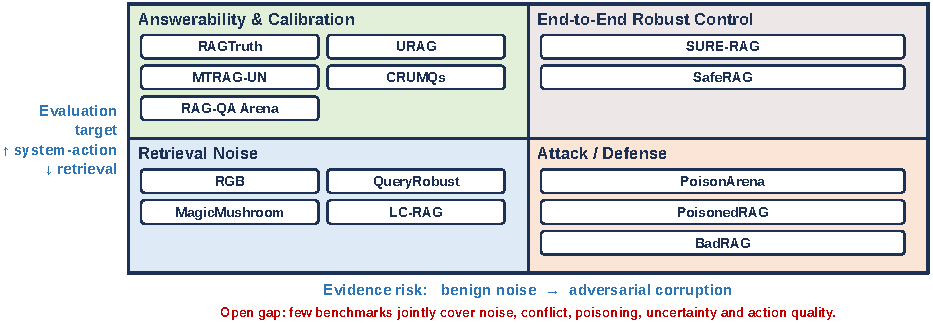
\includegraphics[width=\textwidth]{figures/generated/fig_benchmark_landscape.pdf}%
\caption{Conceptual benchmark landscape. Placement is illustrative rather than
data-derived; the figure organises differences in evidence risk and evaluation
level, not empirical distance or benchmark quality. The two axes are
coordinates C1 and C4, and the open gap is the reason a single ``robustness''
number rarely transfers between quadrants.}
\label{fig:benchmark-landscape}
\end{figure*}

\begin{table*}[t]
\centering
\scriptsize
\renewcommand{\arraystretch}{0.95}
\begin{tabularx}{\linewidth}{>{\raggedright\arraybackslash}p{0.12\linewidth}>{\raggedright\arraybackslash}p{0.13\linewidth}>{\raggedright\arraybackslash}p{0.17\linewidth}>{\raggedright\arraybackslash}p{0.18\linewidth}>{\raggedright\arraybackslash}p{0.14\linewidth}X}
\toprule
\textbf{Benchmark} & \textbf{Risk focus} & \textbf{Task / data} & \textbf{Perturbation or threat} & \textbf{Metrics} & \textbf{Boundary} \\
\midrule
RGB \citep{rgb2023} & noise, rejection, integration, counterfactuality & English/Chinese QA & noisy passages, false evidence, negative evidence & accuracy, ability-specific scores & Broad diagnostic benchmark but not adaptive attack-oriented. \\
RAGTruth \citep{ragTruth2024} & hallucination / faithfulness & QA, data-to-text, summarization & naturally generated unsupported spans & word-level hallucination labels & Strong annotation granularity; less focused on retrieval-side threat models. \\
Sufficient Context \citep{sufficientContext2024} & answerability & QA with context sufficiency labels & insufficient retrieved evidence & selective generation / abstention & Captures answerability but not adversarial corruption. \\
MagicMushroom \citep{rrag027} & retrieval noise & configurable RAG stress tests & distracting, low-quality, inconsequential, irrelevant noise & robustness under noise types & Fine-grained noise; limited conflict/security coverage. \\
URAG \citep{rrag001} & uncertainty & RAG as MCQA / conformal prediction & irrelevant/noisy retrieval and uncertainty sets & coverage, set size, calibration & Good for uncertainty; less direct for free-form generation. \\
QueryRobust \citep{queryRobustness2025} & query robustness & QA with query perturbations & wording variation at query--retrieval interface & retrieval and end-task degradation & Focuses on query perturbation, not corpus corruption. \\
PoisonArena \citep{rrag023} & adversarial poisoning & RAG attack competition setting & competing poisoning attacks & attack success, retrieval effects & Strong security focus; benign uncertainty is secondary. \\
SafeRAG \citep{rrag019} & RAG security & security benchmark for RAG & poisoning / malicious retrieval contexts & attack and defense metrics & Security-oriented; not a full evidence reliability suite. \\
MTRAG-UN \citep{rrag141} & multi-turn unanswerability & multi-turn RAG conversations & unanswerable, underspecified, non-standalone questions & abstention / clarification quality & Covers interaction; less focused on adversarial evidence. \\
CRUMQs \citep{rrag193} & unanswerable multi-hop RAG & realistic multi-hop queries & unanswerable and uncheatable questions & answerability and robustness & Useful for abstention; not a broad attack/noise benchmark. \\
\bottomrule
\end{tabularx}
\caption{Benchmark-level comparison for robust RAG evaluation. The table makes explicit what each benchmark perturbs, what it measures, and which failure modes remain outside its scope.}
\label{tab:benchmark-comparison}
\end{table*}


\begin{table*}[t]
\centering
\scriptsize
\begin{tabularx}{\linewidth}{p{0.18\linewidth}p{0.22\linewidth}p{0.24\linewidth}X}
\toprule
\textbf{Benchmark component} & \textbf{Required annotation} & \textbf{Metric suite} & \textbf{Why it is needed} \\
\midrule
Evidence reliability & relevance, sufficiency, freshness, provenance, support span & retrieval recall, sufficient-context accuracy, support precision & Distinguishes merely related passages from answer-supporting evidence. \\
Distraction and conflict & distractor type, conflicting claim pair, source agreement & answer flip rate, conflict sensitivity, context-utilisation score & Reveals whether models ignore harmful context or silently pick a source. \\
Adversarial corruption & attacker access, insertion budget, trigger type, poisoned document ID & attack success, poisoned retrieval rate, stealth, defense bypass & Makes security results comparable across threat models. \\
Unanswerability and ambiguity & answerability label, ambiguity type, clarification target & selective risk, abstention precision/recall, clarification accuracy & Evaluates robust action selection, not just answer generation. \\
Cost and system action & number of retrievals, verifier calls, latency, final action trace & cost-adjusted accuracy, action utility, coverage--risk curve & Prevents methods from hiding robustness gains behind unbounded computation. \\
\bottomrule
\end{tabularx}
\caption{A proposed benchmark blueprint for robust RAG under unreliable evidence. This is a research agenda rather than a validated leaderboard; existing benchmarks cover parts of the schema.}
\label{tab:benchmark-blueprint}
\end{table*}

\begin{table*}[t]
\centering
\scriptsize
\renewcommand{\arraystretch}{0.88}
\begin{tabularx}{\linewidth}{>{\raggedright\arraybackslash}p{0.16\linewidth}>{\raggedright\arraybackslash}p{0.20\linewidth}>{\raggedright\arraybackslash}p{0.20\linewidth}>{\raggedright\arraybackslash}p{0.18\linewidth}X}
\toprule
\textbf{Pilot item type} & \textbf{Evidence state label} & \textbf{Correct action trace} & \textbf{Answer metric alone would say} & \textbf{Action-aware diagnosis} \\
\midrule
Benign hard negative & Gold evidence present; hard negative ranked above it & retrieve $\rightarrow$ rerank/filter $\rightarrow$ answer with support & Correct/incorrect answer & Separates retriever ranking error from generator distraction. \\
Insufficient context & Retrieved context related but lacks answer-bearing span & retrieve $\rightarrow$ detect insufficiency $\rightarrow$ re-retrieve or abstain & Wrong answer or refusal & Rewards abstention/retrieval control rather than forced guessing. \\
Retrieved conflict & Two sources disagree with different dates/provenance & retrieve $\rightarrow$ compare sources $\rightarrow$ expose conflict or prefer fresher source & One answer may match gold & Checks whether the system hides unresolved conflict. \\
Poisoned evidence & Malicious document retrieved with plausible support & retrieve $\rightarrow$ detect/demote/quarantine $\rightarrow$ answer or abstain & Attack success/failure & Distinguishes poisoned retrieval, defense detection, and final answer steering. \\
\bottomrule
\end{tabularx}
\caption{Illustrative action-trace pilot for the benchmark blueprint. This is a worked annotation example, not a released leaderboard or empirical system ranking.}
\label{tab:action-trace-pilot}
\end{table*}


\begin{table}[t]
\centering
\small
\begin{tabular}{lrrr}
\toprule
\textbf{Toy policy} & \textbf{Ans.} & \textbf{Act.} & \textbf{Joint} \\
\midrule
Answer-only & 0.25 & 0.25 & 0.25 \\
Abstain-on-missing & 0.67 & 0.50 & 0.50 \\
Evidence-action oracle & 1.00 & 1.00 & 1.00 \\
\bottomrule
\end{tabular}
\caption{Action-trace pilot over 12 synthetic diagnostic items. Answer accuracy, action accuracy, and joint answer-action accuracy diagnose different behavior.}
\label{tab:action-trace-pilot-results}
\end{table}


\begin{table*}[t]
\centering
\scriptsize
\renewcommand{\arraystretch}{0.92}
\begin{tabularx}{\linewidth}{>{\raggedright\arraybackslash}p{0.17\linewidth}>{\raggedright\arraybackslash}p{0.27\linewidth}>{\raggedright\arraybackslash}p{0.25\linewidth}X}
\toprule
\textbf{Axis} & \textbf{Typical variation across papers} & \textbf{Why conclusions fail to transfer} & \textbf{Minimum reporting requirement} \\
\midrule
Retriever/generator setting & BM25 vs dense vs hybrid retrieval; small vs frontier generators; frozen vs fine-tuned models & A defense may work by compensating for one retriever or one model scale rather than solving the failure mode. & Retriever, index, top-$k$, reranker, generator, prompt, decoding, and context length. \\
Attack budget and access & Poisoned-document count, corpus write access, query control, retriever visibility, generator access & Attack success rates are incomparable when one attacker edits a corpus and another only controls the query. & Capability matrix, insertion budget, target set, stealth objective, and whether malicious evidence is retrieved. \\
Metric target & EM/F1, faithfulness, citation support, attack success, calibration error, selective risk, cost & Improving answer accuracy can worsen citation faithfulness; improving abstention can reduce coverage; reducing attacks can lower utility. & Report utility, evidence support, risk, calibration, cost, and security as a Pareto surface. \\
Statistical and reproducibility evidence & Single seed/model vs multiple seeds/models; code/data availability varies & Small prompt or model changes can reverse robustness rankings, especially for LLM-as-judge or attack benchmarks. & Seeds, confidence intervals or bootstrap tests where feasible, released prompts, data splits, and code or exact API settings. \\
Long-context baseline & RAG-only comparisons vs long-context LLMs with the same documents & A robustness gain may reflect retrieval compression rather than evidence reliability control. & Include a long-context or full-context baseline when context length permits, and report latency/cost. \\
Attribution vs answer accuracy & Some tasks score only final answer; others require evidence-supported citations & A model can answer correctly for the wrong reason, cite irrelevant evidence, or ignore retrieved support. & Claim-level support labels, citation precision/recall, and answer correctness reported separately. \\
\bottomrule
\end{tabularx}
\caption{Evaluation-assumption matrix for robust RAG. The table summarises why benchmark results often cannot be compared without aligning system setup, threat model, metric target, reproducibility evidence, and long-context baselines.}
\label{tab:evaluation-assumption-matrix}
\end{table*}



Evaluation must reflect the full hierarchy. Standard exact match, F1, and retrieval recall remain useful but insufficient. A RAG system can retrieve relevant evidence and still answer from a distractor; it can answer correctly but be overconfident; it can refuse correctly but fail to explain what evidence is missing; it can pass benign noise tests but fail under poisoned corpora. Robust evaluation must therefore measure both failure resistance and action quality.

We group robust RAG evaluation into six families:
\begin{enumerate}[leftmargin=*]
    \item \textbf{Noise robustness}: performance as irrelevant or misleading passages are injected, removed, reordered, or ranked higher.
    \item \textbf{Distraction sensitivity}: whether answer or confidence changes when distractors are added while gold evidence remains available.
    \item \textbf{Conflict sensitivity}: whether the system detects and resolves parametric--retrieved or retrieved--retrieved contradictions.
    \item \textbf{Adversarial robustness}: attack success rate, poisoned retrieval rate, trigger robustness, defense bypass rate, and recovery after filtering.
    \item \textbf{Uncertainty and selective prediction}: selective risk, abstention precision/recall, expected calibration error, and clarification quality.
    \item \textbf{End-to-end action quality}: whether the system chooses the right policy among answer, retrieve, re-retrieve, filter, abstain, or ask.
\end{enumerate}
Benchmarking work such as RGB, RAGTruth, robustness-at-query-level analyses, poisoning benchmarks, and uncertainty benchmarks provides pieces of this landscape \citep{rgb2023,ragTruth2024,queryRobustness2025}. RGB is useful because it separates RAG abilities rather than reporting one score \citep{rgb2023}. RAGTruth contributes fine-grained hallucination annotations that support detection and attribution \citep{ragTruth2024}. Query-level robustness work shows that the query--retrieval interface is itself fragile \citep{queryRobustness2025}. PoisonArena-style benchmarks and LIAR-style attack evaluations stress adversarial settings rather than benign retrieval noise \citep{rrag023,rrag035}. URAG and uncertainty benchmarks evaluate whether systems know when their answers are reliable \citep{rrag001,rrag093}.

The main gap is joint evaluation. Most benchmarks isolate one failure: noise, conflict, poisoning, or unanswerability. In plausible high-risk document-grounded settings, these failures can interact: a query may be ambiguous, retrieval may surface partially relevant evidence, a document may be stale, and one source may be malicious or misleading. A future benchmark should therefore cross product failure types: benign hard negatives, conflicting evidence, poisoned passages, query perturbations, and insufficient context. It should also report action metrics: when the system retrieves, when it filters, when it verifies, when it abstains, and whether these actions improve risk--cost tradeoffs.

Table~\ref{tab:benchmark-blueprint} turns this observation into a proposed benchmark schema. We treat it as a research agenda, not as a validated benchmark contribution: no leaderboard or empirical re-ranking is claimed. The key design choice is to annotate not only answers but also evidence states and action traces. Without evidence annotations, a model can receive credit for an answer supported by parametric memory rather than retrieved evidence. Without action traces, a system that repeatedly retrieves, verifies, and self-consistently samples can look more robust while hiding its cost. Without attacker capability fields, security benchmark results become incomparable.

To make the proposal concrete, we include a 12-item synthetic action-trace pilot with three toy policies (Table~\ref{tab:action-trace-pilot-results}). The pilot is not a benchmark release, but it demonstrates the diagnostic difference: an answer-only policy can receive some answer credit while failing action quality, whereas action-aware scoring distinguishes answer correctness, control behavior, and their joint success.

Table~\ref{tab:evaluation-assumption-matrix} makes the comparison problem more explicit. Many reported gains depend on retriever choice, generator scale, context length, poisoning budget, and metric target. A method can improve EM while worsening citation support; a defense can reduce attack success while reducing answer utility; a retrieval policy can increase accuracy while hiding cost. We therefore treat robust-RAG evaluation as a multi-axis reporting problem rather than a leaderboard scalar.

\paragraph{A concrete benchmark protocol.}
An executable robust-RAG benchmark should instantiate the following template. Each item contains a user query, a gold answer or abstention/clarification target, a corpus snapshot with document IDs, a retrieved-context candidate set, and labels for supporting, distracting, conflicting, stale, poisoned, and insufficient evidence. The benchmark should define four splits: benign retrieval noise, knowledge conflict, adversarial corruption, and answerability uncertainty. For each split, systems must output both an answer and an action trace: whether they retrieved, filtered, verified, re-retrieved, abstained, or asked for clarification. The metric suite should report answer utility, evidence support precision, attack success or defense bypass where applicable, calibration/coverage, and cost-adjusted action utility. This protocol makes it possible to compare systems that answer directly against systems that spend additional computation on verification or abstention.

\paragraph{Metric Design}

Robust RAG metrics should be diagnostic. For retrieval, recall and nDCG should be complemented by negative-utility metrics that penalise distracting evidence \citep{rrag058}. For generation, exact match should be complemented by faithfulness, citation support, and claim-level entailment. For attacks, attack success rate should be paired with stealth, retrieval rate, injected-document budget, and transferability. For calibration, expected calibration error should be paired with selective risk and coverage. For control, the unit of evaluation should be an action trace: retrieve, filter, verify, answer, abstain, or ask clarification. This makes it possible to distinguish a lucky correct answer from a robust decision process.

\paragraph{Benchmark Construction Principles}

We identify four principles for future benchmark construction. First, benchmarks should include both benign and adversarial evidence unreliability. Second, they should provide source-level annotations: which passage supports which claim, which passage is distracting, which passage is poisoned, and which source conflicts with which. Third, they should include unanswerable and underspecified questions so that abstention and clarification can be evaluated. Fourth, they should report cost and latency, because robust RAG methods often trade reliability for additional computation. Benchmarks that omit these dimensions risk rewarding systems that answer more often rather than systems that answer more responsibly.


\FloatBarrier
\section{Cross-Cutting Analysis}
\label{app:crosscut}
\begin{table*}[t]
\centering
\scriptsize
\renewcommand{\arraystretch}{0.9}
\begin{tabularx}{\linewidth}{>{\raggedright\arraybackslash}p{0.18\linewidth}>{\raggedright\arraybackslash}p{0.25\linewidth}>{\raggedright\arraybackslash}p{0.23\linewidth}X}
\toprule
\textbf{Backbone conclusion} & \textbf{Venue-linked evidence base} & \textbf{What remains stable} & \textbf{What remains preprint/trend evidence} \\
\midrule
Irrelevant or noisy evidence can change generation behavior. & Irrelevant-context robustness, noise-aware training, counterfactual-noise analyses, and robust fine-tuning papers in ICLR/ACL/NAACL/SIGIR-style venues. & Robustness is not just retriever recall; generator selectivity and context construction matter. & Fine-grained noise taxonomies, long-tail stress tests, and model-specific mitigation rankings. \\
Knowledge conflict is distinct from poisoning. & Conflict-resolution and imperfect-retrieval work in TACL/COLING/EMNLP-style records, plus venue-linked conflict benchmarks. & Natural contradiction requires source reconciliation and evidence sufficiency reasoning. & Many automatic conflict-resolution methods and large-scale conflict benchmark variants. \\
RAG security comparisons require capability normalisation. & USENIX/WWW/CCS/KDD-style poisoning, traceback, membership-inference, and backdoor records. & Attack success cannot be interpreted without corpus write access, query control, retriever visibility, insertion budget, and stealth. & The detailed ranking of attacks/defenses and many newly proposed bypasses. \\
Calibration and abstention are action-control decisions. & Venue-linked relevance-assessment, answerability, calibration, and RAG evaluation records. & Confidence, evidence sufficiency, retrieve/answer decisions, and abstention are separable evaluation targets. & Specific adaptive-control policies and frontier-model calibration behavior. \\
Benchmark design needs evidence and action labels. & RGB, RAGTruth, RAG evaluation libraries, long-form/context benchmarks, and challenge-style records. & Answer accuracy alone is insufficient for robust RAG evaluation. & The full action-trace blueprint remains a proposal until implemented and validated. \\
\bottomrule
\end{tabularx}
\caption{Peer-reviewed / venue-linked backbone of the analysis. These are the conclusions the paper treats as stable when preprint-only evidence is downweighted.}
\label{tab:peer-reviewed-backbone}
\end{table*}


\begin{table*}[t]
\centering
\scriptsize
\renewcommand{\arraystretch}{0.82}
\begin{tabularx}{\linewidth}{>{\raggedright\arraybackslash}p{0.17\linewidth}>{\raggedright\arraybackslash}p{0.25\linewidth}>{\raggedright\arraybackslash}p{0.24\linewidth}X}
\toprule
\textbf{Case} & \textbf{Naive reading} & \textbf{Normalization coordinate that changes it} & \textbf{Revised conclusion} \\
\midrule
IrrelCtx \citep{irrelevantContext2023} vs. RAAT \citep{raat2024} & Both are ``noise-robust RAG'' methods. & IrrelCtx targets naturally retrieved irrelevant context and filtering/back-off; RAAT trains on constructed relevant/irrelevant/counterfactual mixtures. & They are complementary context-filtering vs. noise-training regimes, not one leaderboard. \\
IrrelCtx \citep{irrelevantContext2023} vs. Chain-of-Note \citep{chainOfNote2023} & Both reduce distractor harm. & Intervention point differs: context filtering/fine-tuning vs. generator-side document reading. & A valid comparison must hold context state fixed and report whether the action is filter, answer, or unknown. \\
Sufficient Context \citep{sufficientContext2024} vs. Self-RAG \citep{selfRAG2023} & Both decide when retrieval is useful. & Evidence-sufficiency labeling vs. retrieve/generate/critique action policy. & Sufficiency prediction is an evidence-state signal; adaptive retrieval is a policy over actions and costs. \\
RAGTruth \citep{ragTruth2024} vs. FaithfulRAG/AstuteRAG \citep{faithfulRAG2025,astuteRAG2025} & All are faithfulness/conflict papers. & Unit of support differs: generated span support vs. fact/source conflict resolution. & Detector F1 and conflict-resolution accuracy should not be pooled as one faithfulness score. \\
Tug-of-War \citep{tugOfWar2024} vs. ParamMute \citep{rrag024} & Both study parametric-vs-contextual knowledge. & Source-preference analysis vs. parametric-knowledge suppression/intervention. & The conclusion shifts from ``trust context or model'' to reporting source reliability and update policy. \\
Poisoning corpora \citep{poisoningRetrievalCorpora2023} vs. PoisonedRAG \citep{poisonedRAG2024} & Both are RAG poisoning attacks. & Corpus-write access, query control, retriever visibility, and target objective differ. & Attack success rates transfer only inside a shared capability envelope. \\
PoisonedRAG \citep{poisonedRAG2024} vs. CertifiedRAG \citep{certifiedRAG2024} & Attack and defense appear directly comparable. & Defense guarantee assumes bounded retrieved corruption and an aggregation/abstention policy. & Certification is meaningful only under the stated budget; it is not a universal defense to open-web insertion. \\
AgentPoison \citep{rrag053} vs. document poisoning \citep{poisonedRAG2024} & Both corrupt retrieved evidence. & Persistent memory/tool state vs. static corpus passages. & Agentic poisoning needs memory-update and tool-call action labels, not only answer steering. \\
Spill-Beans/privacy \citep{venue200SpillBeans} vs. steering attacks \citep{poisonedRAG2024} & Both are security failures. & Objective differs: data extraction or privacy leakage vs. answer manipulation. & Privacy, extraction, steering, traceback, and recovery require separate outcome columns. \\
RAGAS/ARES \citep{ragas2024,ares2024} vs. RAGTruth \citep{ragTruth2024} & All evaluate grounded RAG. & LLM-as-judge metric toolkit vs. human-annotated hallucination/support resource. & Automated evaluation and corpus labels are different evidence artifacts; agreement with one does not validate the other. \\
RGB \citep{rgb2023} vs. Sufficient Context \citep{sufficientContext2024} & Both benchmark unreliable evidence. & Diagnostic ability axes vs. answerability/sufficiency labels and selective risk. & A benchmark score is interpretable only after stating the evidence state and required action. \\
Lost-in-the-Middle \citep{liu2024lostmiddle} vs. long-context retrieval & More context seems to solve retrieval misses. & Evidence availability differs from evidence selection and citation. & Full-context access can still fail if the model cannot select or ground the supporting span. \\
ColPali/Table/Graph RAG \citep{colpali2025,tableRAG2024,venueAcc004} vs. passage RAG & Extension papers look like new application areas. & Evidence object changes: page image, table cell/schema, graph neighborhood, or tool memory. & They are retained as extension-layer stress tests of typed evidence states, not as broad co-equal survey scope. \\
\bottomrule
\end{tabularx}
\caption{Concrete conclusions that change after five-coordinate normalization. Each row is grounded in released case-study or Map-B records and shows why a common citation-list comparison becomes invalid, partial, or more specific once failure, assumption, intervention, metric, and action are aligned.}
\label{tab:main-normalization-findings}
\end{table*}


% Drawn by scripts/revision3/fig_appendix_schematics.py; the .pptx is the
% editable source and is released with the paper.
\begin{figure*}[t]
\centering
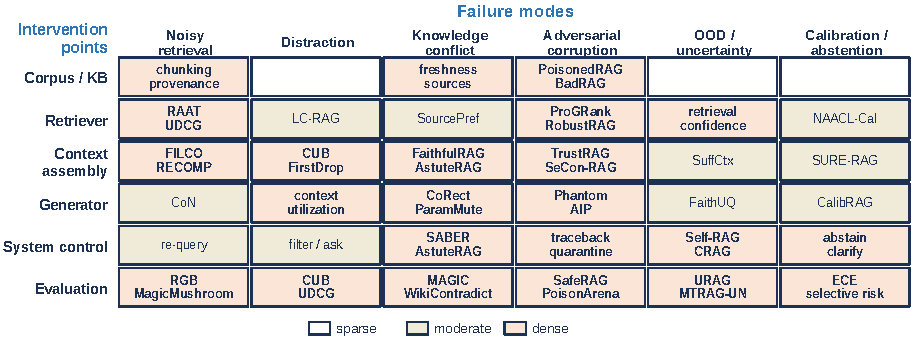
\includegraphics[width=\textwidth]{figures/generated/fig_failure_matrix.pdf}%
\caption{Schematic literature-family $\times$ intervention matrix. Shading and
example labels are illustrative design aids, not counts from Map~B;
quantitative Map-B distributions appear in Table~\ref{tab:corpus-stats}. Rows
are coordinate C3 and columns are coordinate C1, which is why a cell, not a
column, is the unit at which two systems become comparable.}
\label{fig:failure-intervention-matrix}
\end{figure*}

\begin{table*}[t]
\centering
\scriptsize
\renewcommand{\arraystretch}{0.92}
\begin{tabularx}{\linewidth}{>{\raggedright\arraybackslash}p{0.13\linewidth}>{\raggedright\arraybackslash}p{0.12\linewidth}>{\raggedright\arraybackslash}p{0.16\linewidth}>{\raggedright\arraybackslash}p{0.18\linewidth}>{\raggedright\arraybackslash}p{0.13\linewidth}>{\raggedright\arraybackslash}X}
\toprule
\textbf{Work} & \textbf{Failure} & \textbf{Task / setup} & \textbf{Key assumption} & \textbf{Metric} & \textbf{Boundary} \\
\midrule
IrrelCtx & irrelevant context & Open-domain QA & Irrelevance can be filtered or learned against & Robust accuracy & No adversarial/conflict setting. \\
RAAT & retrieval noise & Noisy QA training & Noise-aware training improves generation & F1/EM & Needs deployment-like noise. \\
RGB & multi-ability RAG & Bilingual benchmark & RAG reliability decomposes into abilities & Ability accuracy & Not adversarially adaptive. \\
FaithfulRAG & conflict & Fact-level conflict & Conflicts can be localised and reasoned over & Faithfulness & Needs reliable fact extraction. \\
AstuteRAG & imperfect retrieval & Training-free consolidation & Internal/external knowledge can be reliability-compared & Robust QA & Depends on LLM self-assessment. \\
PoisonedRAG & poisoning & Injected passages & Few crafted passages can dominate retrieval & Attack success & Targeted corruption focus. \\
RobustRAG & defense & Bounded corruption & Isolate-and-aggregate can certify robustness & Certificate, accuracy & Assumes attack budget. \\
Self-RAG / CtrlA & adaptive retrieval & Retrieve-or-answer & Model state can trigger retrieval & Trigger quality & Calibration can shift. \\
CalibRAG / URAG & calibration & Decision/MCQA & Confidence should reflect evidence uncertainty & ECE, coverage & Does not repair evidence. \\
PoisonArena / SafeRAG & security eval. & Poisoning benchmark & Threat models must be explicit & ASR, bypass & Still isolates attacks. \\
\bottomrule
\end{tabularx}
\caption{Analytical matrix of representative robust RAG work. Compared with a citation list, the matrix highlights each work's task setup, central assumption, metric focus, and boundary of applicability.}
\label{tab:analytical-matrix}
\end{table*}

\begin{table*}[t]
\centering
\scriptsize
\renewcommand{\arraystretch}{0.86}
\begin{tabularx}{\linewidth}{>{\raggedright\arraybackslash}p{0.13\linewidth}>{\raggedright\arraybackslash}p{0.17\linewidth}>{\raggedright\arraybackslash}p{0.17\linewidth}>{\raggedright\arraybackslash}p{0.16\linewidth}>{\raggedright\arraybackslash}p{0.13\linewidth}X}
\toprule
\textbf{Work} & \textbf{System setup} & \textbf{Failure construction} & \textbf{Metric / cost} & \textbf{Main claim} & \textbf{Failure boundary} \\
\midrule
IrrelCtx & RALM / open-domain QA; retrieved context injected into generator & Irrelevant passages with varying plausibility & Robust accuracy / answer degradation & Models can be brittle to irrelevant context. & Does not cover adversarial corruption or answerability policy. \\
RAAT & Noise-aware training for retrieval-augmented LMs & Multiple retrieval-noise types during training/evaluation & EM/F1 under noisy retrieval & Adaptive adversarial training improves noise robustness. & Transfer depends on whether deployment noise matches training noise. \\
RGB & Benchmark over English/Chinese QA-style RAG tasks & Noise, negative rejection, integration, counterfactual evidence & Ability-specific accuracy & RAG reliability decomposes into distinct abilities. & Benchmark abilities are diagnostic but not a unified control policy. \\
Sufficient Context & QA contexts labeled by sufficiency & Insufficient vs sufficient retrieved evidence & Selective answering / abstention quality & Evidence sufficiency should govern answerability. & Does not repair retrieval and does not model adversarial evidence. \\
PoisonedRAG & Corpus-injection attack against RAG & Crafted poisoned passages inserted into retrieval corpus & Attack success, retrieval of poison & Few poisoned documents can steer answers. & Strength depends on corpus write access, topic targeting, and retrieval success. \\
Certified / isolate defenses & Bounded-corruption RAG defense setting & Assumed corruption budget over retrieved evidence & Certificate, robust accuracy & Aggregation can certify robustness under budget assumptions. & Guarantees narrow when attacker violates budget or attacks instructions/tools. \\
Self-RAG / CtrlA & Adaptive retrieve-or-answer policies & Uncertainty about whether retrieval is needed & Trigger quality, answer utility, cost & Retrieval should be a conditional action. & Calibration shifts under distribution change; action cost often underreported. \\
RAGTruth & Annotated hallucination/faithfulness resource & Naturally generated unsupported spans across tasks & Span-level hallucination labels & Fine-grained support labels improve evaluation. & Faithfulness labels do not fully specify retrieval failure or system action. \\
\bottomrule
\end{tabularx}
\caption{Method-level comparison of representative robust-RAG work. The table makes explicit the setup, failure construction, metric target, main claim, and failure boundary that must be aligned before comparing methods.}
\label{tab:method-level-comparison}
\end{table*}


\begin{table*}[t]
\centering
\scriptsize
\renewcommand{\arraystretch}{0.86}
\begin{tabularx}{\linewidth}{>{\raggedright\arraybackslash}p{0.14\linewidth}>{\raggedright\arraybackslash}p{0.19\linewidth}>{\raggedright\arraybackslash}p{0.24\linewidth}>{\raggedright\arraybackslash}p{0.18\linewidth}X}
\toprule
\textbf{Case} & \textbf{Released rows / papers} & \textbf{Audited comparison fields} & \textbf{Metric or failure conflict} & \textbf{Synthesis / artifact boundary} \\
\midrule
Noise / distraction robustness & 5 rows: IrrelCtx, RAAT, Chain-of-Note, Sufficient Context, RGB & Assumption, QA dataset or benchmark slice, generator / reader setup, negative type, rank and gold-evidence availability. & EM/F1, rejection, selective risk, and ability-specific benchmark scores answer different questions. & Treat filtering, noise-aware training, generator reading, sufficiency prediction, and benchmark diagnosis as different mechanisms; artifact status is recorded per paper in the released worksheet. \\
Faithfulness, conflict, and attribution & 5 rows: RAGTruth, FaithfulRAG, AstuteRAG, Tug-of-War, Chain-of-Note & Unit of support, source-conflict assumption, attribution granularity, model-side reasoning setup, artifact availability. & Span-level support, fact-level conflict resolution, source preference, and final answer accuracy can disagree. & Citation faithfulness should not be collapsed into conflict robustness; the worksheet records where artifact evidence is dataset-level, code-level, or paper-only. \\
Adversarial corruption and RAG security & 6 rows: PoisonedRAG, corpus poisoning, BadRAG, certified defense, TrojanRAG, traceback & Corpus write access, insertion budget, retriever visibility, query control, generator access, stealth, retrieved malicious evidence, defense timing. & Attack success, certified robust accuracy, detection, traceback, and clean utility are not one defense score. & Compare only inside a capability envelope; prevention, demotion, detection, traceback, recovery, and certification remain separate outcomes. \\
Calibration, abstention, and adaptive control & 5 rows: Sufficient Context, Self-RAG, CRAG, CalibRAG, uncertainty RAG & Confidence target, evidence sufficiency labels, retrieval trigger, action set, cost budget, model/policy setup. & ECE, selective risk, coverage, retrieval-trigger quality, and answer utility can move in different directions. & Separate belief estimation from action selection; report coverage, cost, and final action alongside correctness. \\
Evaluation and benchmark comparability & 5 rows: RGB, RAGTruth, Sufficient Context, query robustness, RAG security benchmark & Evidence-state labels, perturbation source, model outputs scored, threat model, benchmark artifact availability. & Harder scores may reflect retrieval instability, unsupported spans, unanswerability, or adversarial steering. & Evaluation resources are diagnostic slices, not a universal robustness scale; benchmark comparisons require aligned evidence state and action policy. \\
\bottomrule
\end{tabularx}
\caption{Deeper case-study synthesis. The released 26-row worksheet compares assumptions, datasets or benchmark settings, model/evidence setup, metrics, failure modes, artifact availability, and comparison implications for the same five C1--C5 cases.}
\label{tab:deep-case-study-matrix}
\end{table*}

\begin{table*}[t]
\centering
\scriptsize
\renewcommand{\arraystretch}{0.9}
\begin{tabularx}{\linewidth}{>{\raggedright\arraybackslash}p{0.19\linewidth}>{\raggedright\arraybackslash}p{0.24\linewidth}>{\raggedright\arraybackslash}p{0.23\linewidth}X}
\toprule
\textbf{Apparent conclusion} & \textbf{What the framework changes} & \textbf{Non-trivial finding} & \textbf{Implication} \\
\midrule
``Method A is more robust to noise than method B.'' & Aligns noise type, rank position, gold-evidence availability, and intervention point. & Some methods solve generator distraction while others solve retriever defects; their scores are not competing estimates of the same property. & Report noise source and intervention point before ranking methods. \\
``Defense X lowers attack success.'' & Separates prevention, demotion, detection, traceback, and recovery. & A defense can improve traceback without lowering user-facing attack success, or certify bounded corruption without handling prompt-bearing documents. & Security papers should report outcome type, not only attack success rate. \\
``Calibration improves reliability.'' & Separates confidence in answer correctness from evidence sufficiency and action utility. & A calibrated answerer can still answer from insufficient evidence; an abstaining system can lower risk while reducing coverage. & Calibration metrics should be paired with evidence and action metrics. \\
``Benchmark Y is harder.'' & Compares evidence state, required action, cost budget, and metric target. & A benchmark can be hard because retrieval fails, because evidence conflicts, or because the correct action is refusal; these failures should not be pooled. & Leaderboards should expose diagnostic sub-scores instead of one robust-RAG score. \\
\bottomrule
\end{tabularx}
\caption{Distilled classes of non-trivial findings produced by the comparability framework. Main Table~\ref{tab:main-normalization-findings} gives the concrete paper-pair cases; this appendix table groups them into reusable interpretation rules.}
\label{tab:nontrivial-findings}
\end{table*}

\begin{table*}[t]
\centering
\scriptsize
\renewcommand{\arraystretch}{0.9}
\begin{tabularx}{\linewidth}{>{\raggedright\arraybackslash}p{0.24\linewidth}>{\raggedright\arraybackslash}p{0.25\linewidth}>{\raggedright\arraybackslash}p{0.21\linewidth}X}
\toprule
\textbf{Main claim} & \textbf{Cited evidence basis} & \textbf{What the evidence supports} & \textbf{Boundary} \\
\midrule
Irrelevant or noisy context can harm generation. & Irrelevant-context robustness, RAAT, RGB, and counterfactual-noise studies. & Noise affects both retrieval quality and generator context use. & Does not imply one robustness score covers all noise types. \\
Knowledge conflict differs from adversarial corruption. & Conflict and poisoning studies with different evidence origins and evaluation targets. & Natural disagreement and attacker-created contradiction require different assumptions. & Conflict-resolution results should not be read as poisoning-defense results. \\
RAG attacks require capability normalisation. & Poisoning, backdoor, prompt-injection, traceback, and certification studies. & Attack/defense results require corpus access, query control, retriever visibility, and budget. & The paper does not rank attacks by real-world prevalence. \\
Calibration, abstention, and retrieval control are distinct. & Sufficient-context, uncertainty, adaptive-retrieval, and calibration studies. & Confidence estimation, evidence sufficiency, retrieval triggering, and abstention optimise different quantities. & Does not validate a single universal control policy. \\
Action-trace evaluation is a benchmark agenda. & Benchmarks exposing subsets of answer, evidence, action, cost, and threat fields. & Existing benchmarks cover pieces of the proposed schema. & No new leaderboard or empirical system ranking is claimed. \\
\bottomrule
\end{tabularx}
\caption{Narrative claim-to-source ledger. Expanded and strict citation audits
were model-assisted and deterministic; this table records the intended evidence
boundary rather than certifying every citation.}
\label{tab:claim-verification-ledger}
\end{table*}


\paragraph{Peer-Reviewed Backbone and Preprint Trends}

The main synthesis is anchored in the venue-linked backbone summarised in Table~\ref{tab:peer-reviewed-backbone}. Under that stricter evidence stratum, five conclusions remain stable: retrieved evidence can harm generation; conflict and poisoning require different assumptions; security results require attacker-capability normalisation; calibration and abstention are separate control decisions; and answer accuracy alone is insufficient for robust-RAG evaluation. The broader 268-paper adjudicated map is still useful, but mainly for trend discovery and auditability. Its preprint-heavy cross-tabs are moved to Appendix~\ref{sec:map-statistics}; they diagnose where the map is dense or sparse, but they are not used as field-wide prevalence estimates.

\paragraph{Critical judgments from the re-analysis.}
The framework weakens three common readings of the literature. First, many ``robust to retrieval noise'' claims are over-broad: once distractor hardness, gold-evidence availability, and intervention point are aligned, several methods address complementary mechanisms rather than competing on one robustness axis. Second, many RAG security defenses are narrower than their abstracts suggest: a defense against bounded factual corruption is not evidence of robustness to prompt-bearing documents, trigger-based backdoors, or post-hoc traceback settings. Third, answer-only benchmark gains are often under-specified: without citation support, evidence sufficiency, and action-cost labels, a higher score can mean better answering, riskier coverage, or simply more computation. These are the places where the framework changes interpretation rather than merely renaming categories.

\paragraph{Where Robustness Interventions Act}

Across the literature, robustness interventions cluster by where they act in the RAG pipeline. \textbf{Corpus-level interventions} sanitise, filter, watermark, or validate documents before indexing. They are attractive because they prevent bad evidence from entering the system, but they require corpus governance and may not be possible for open-web retrieval. \textbf{Retriever-level interventions} improve ranking, detect poisoned passages, or diversify evidence. They are efficient and model-agnostic, but they only control what enters the context, not how the generator uses it. \textbf{Context-level interventions} compress, reorder, or filter the retrieved context. They are flexible, but can remove qualifiers or multi-hop evidence. \textbf{Generator-level interventions} use prompting, fine-tuning, note-taking, self-reflection, or hidden-state control. They directly address evidence use but may be model-specific. \textbf{System-level interventions} decide when to retrieve, verify, abstain, or ask. They are closest to deployment needs but require calibrated signals from all earlier stages.

This intervention map helps explain why papers sometimes appear to solve the same problem while actually operating at different layers. For example, irrelevant-context filtering \citep{irrelevantContext2023}, Chain-of-Note \citep{chainOfNote2023}, and Sufficient Context \citep{sufficientContext2024} all address unreliable evidence, but the first filters evidence, the second changes generator reasoning, and the third changes answer policy. Similarly, PoisonedRAG-style attacks \citep{poisonedRAG2024} target the corpus-to-generation path, while AIP attacks prompt templates \citep{aip2025}. A comprehensive survey must therefore compare methods by intervention point, not only by reported task accuracy.

\paragraph{Critical Case Studies of Taxonomy Use}
\begin{table*}[t]
\centering
\scriptsize
\renewcommand{\arraystretch}{0.9}
\begin{tabularx}{\linewidth}{>{\raggedright\arraybackslash}p{0.17\linewidth}>{\raggedright\arraybackslash}p{0.25\linewidth}>{\raggedright\arraybackslash}p{0.25\linewidth}X}
\toprule
\textbf{Case} & \textbf{Papers / settings compared} & \textbf{Why naive comparison fails} & \textbf{Synthesis from the framework} \\
\midrule
Noise / distraction robustness & IrrelCtx, RAAT, RGB, Chain-of-Note, Sufficient Context & Some vary retriever noise, some change generator reading behavior, and some decide answerability; robust accuracy, ability scores, and abstention metrics answer different questions. & Treat retrieval imperfection, harmful context influence, and insufficient evidence as separate states; compare methods only after fixing the intervention point and required action. \\
Faithfulness, conflict, and attribution & RAGTruth, FaithfulRAG, AstuteRAG, Tug-of-War, Chain-of-Note & Span-level support, fact-level conflict, document-level reading, and final answer correctness are different target objects. & Citation faithfulness is not the same as conflict robustness; valid comparisons must state support unit, source reliability assumption, and action policy. \\
Adversarial corruption and RAG security & PoisonedRAG, BadRAG, certified defenses, traceback methods, prompt-injection defenses & One result may assume corpus write access, another bounded corruptions, another instruction-bearing documents, and another post-hoc observability; attack success rates transfer poorly across assumptions. & Report corpus write access, insertion budget, retriever visibility, generator access, stealth, and whether malicious evidence was retrieved before comparing attacks or defenses. \\
Calibration, abstention, and adaptive control & Self-RAG, CRAG, CalibRAG, uncertainty RAG, Sufficient Context & ECE, selective risk, retrieval-trigger quality, and abstention precision measure different objects; better confidence does not necessarily repair evidence or choose the right user action. & Separate belief estimation from action selection. A complete benchmark should score confidence, evidence sufficiency, final action, and cost. \\
Evaluation and benchmark comparability & RGB, RAGTruth, Sufficient Context, query-robustness benchmarks, RAG security arenas & A benchmark can be hard because retrieval fails, evidence conflicts, attribution is unsupported, the item is unanswerable, or an attacker is stronger. & Evaluation resources should expose diagnostic sub-scores and threat/action labels rather than one robust-RAG scalar. \\
\bottomrule
\end{tabularx}
\caption{Critical case studies showing how the comparability framework changes interpretation of representative robust-RAG papers.}
\label{tab:critical-case-studies}
\end{table*}


\paragraph{Case 1: irrelevant evidence is not one problem.}
IrrelCtx, RAAT, RGB, Chain-of-Note, and Sufficient Context are sometimes all described as robustness-to-noise work, but they instantiate different experimental objects. IrrelCtx tests whether a generator can ignore irrelevant context; RAAT treats noise as a training distribution; RGB decomposes reliability into benchmark abilities; Chain-of-Note changes the generator's intermediate reading behavior; Sufficient Context changes the answer policy when evidence is inadequate. A direct leaderboard comparison would mix retrieval perturbation, generator selectivity, and answerability control. The taxonomy changes the question from ``which method is best under noise?'' to ``which evidence state is present, which module intervenes, and what action should be scored?''

\paragraph{Case 2: poisoning papers differ by attacker capability.}
Poisoning Retrieval Corpora, PoisonedRAG, BadRAG, TrojanRAG, Phantom, AIP, and newer one-shot or traceback studies are all adversarial, but they assume different access and objectives. Some manipulate dense retrieval, some steer final answers, some rely on triggers, some attack shared prompt templates, and some evaluate whether poisoned evidence can be traced after the fact. Attack success rate is therefore not a portable metric unless corpus write access, query control, retriever visibility, generator access, insertion budget, and stealth requirements are aligned. This is why Table~\ref{tab:attacker-capability} treats capability fields as part of the result, not just implementation detail.

\paragraph{Case 3: calibration is not the same as abstention.}
UncertaintyRAG, CalibRAG, URAG, Self-RAG, CtrlA, Sufficient Context, and SABER-style trust/abstain methods all relate to uncertainty, but they optimise different objects. Some estimate uncertainty in spans or answer sets; some calibrate decision confidence; some decide when to retrieve; some decide when to abstain; some predict whether the retrieved context is sufficient. Expected calibration error, selective risk, retrieval-trigger accuracy, and abstention precision cannot be collapsed into one number. The taxonomy forces a distinction between belief estimation and action selection, explaining why a method can improve calibration without repairing evidence or improve retrieval triggering without improving final answer faithfulness.

\paragraph{Case 4: poisoning defenses do not share one threat model.}
Certified defenses, isolate-and-aggregate defenses, poisoned-document detectors, activation-based traceback, and prompt-injection defenses respond to different adversarial assumptions. A certificate can be meaningful under a bounded corruption budget but irrelevant when the attacker controls prompt-like instructions; a traceback method may be useful after an incident but may not prevent answer steering; a prompt-injection defense may not address embedding-space poisoning. The framework therefore asks defense papers to report the same capability fields as attack papers and to distinguish prevention, detection, demotion, traceback, and recovery.

\paragraph{Strengths and Weaknesses by Method Family}

Filtering and reranking are attractive robustness methods because they can be added around existing LLMs. Their weakness is false negatives: an aggressive filter may discard the only passage that supports a rare or multi-hop answer. Robust training can teach models to ignore noise, but training data may not cover future attacks or domain-specific distractors. Conflict modeling provides a principled way to handle contradictions, but fact extraction and alignment remain brittle for long, compositional, or numerical claims. Certified defenses provide valuable guarantees, but their assumptions are often narrower than realistic attack surfaces. Adaptive retrieval and abstention improve risk control, but their performance depends on calibration signals that can themselves be miscalibrated under distribution shift.

The synthesis suggests that method families should be composed according to risk profile rather than stacked indiscriminately. A low-risk FAQ system may only justify lightweight filtering and citation checks, while a high-stakes document-grounded setting may require source validation, contradiction detection, selective abstention, and escalation. These are design implications, not claims that the evidence map validates any particular enterprise, medical, or legal deployment.

\paragraph{What Counts as Progress?}

The corpus currently reports progress through heterogeneous metrics: EM/F1, hallucination rate, retrieval recall, attack success rate, calibration error, abstention accuracy, and human preference. These metrics are not directly comparable. A defense that reduces attack success may reduce answer utility; a calibration method may improve selective risk while lowering coverage; a retriever that improves recall may increase distraction. Robust RAG progress should therefore be reported as a Pareto frontier across utility, robustness, calibration, cost, and security. This mirrors the broader lesson from trustworthy ML: robustness is not a scalar property but a tradeoff surface.

\paragraph{What Is Still Missing from the Literature}

Several gaps recur across categories. First, benchmarks rarely combine failures. Noise, conflict, poisoning, and unanswerability are usually tested separately, even though realistic systems may encounter them jointly. Second, many papers evaluate with one retriever and one generator, making transfer difficult to assess. Third, few works evaluate long-term corpus dynamics: documents are updated, poisoned documents are removed, indices are rebuilt, and user feedback changes future retrieval. Fourth, most papers treat users as passive recipients rather than interactive participants who can clarify intent or verify sources. Fifth, multilingual and multimodal robust RAG remains underdeveloped relative to text-only English QA; because our corpus is also text-heavy, this is a boundary of the present survey rather than a resolved conclusion about those areas.


\FloatBarrier
\subsection{Evidence-Map Cross-Tabulations}
\label{sec:map-statistics}
These cross-tabulations diagnose where the released map is dense or sparse. They
are preprint-heavy and are not used anywhere as field-wide prevalence estimates.
\begin{table*}[t]
\centering
\small
\begin{tabularx}{\linewidth}{p{0.18\linewidth}X}
\toprule
\textbf{Dimension} & \textbf{Distribution in the 342-paper adjudicated Map B} \\
\midrule
Publication year & 2025: 170; 2024: 92; 2026: 65; 2023: 12; 2021: 2; 2022: 1 \\
Source / venue type & arXiv/preprint: 207; venue/proceedings-linked: 126; workshop/challenge: 5; other/unclear: 4 \\
Primary failure category & adversarial corruption: 120; knowledge conflict: 57; calibration/control: 55; evaluation/benchmark: 43; noisy retrieval: 34; distraction: 18; extension layer: 7; survey/background: 6; OOD/uncertainty: 2 \\
Method family & defense/mitigation: 119; attack: 75; benchmark/evaluation: 67; control/calibration: 27; method/evaluation: 21; analysis: 21; survey background: 6; conflict modeling: 4; method: 2 \\
Intervention point & generator: 81; corpus/KB: 67; evaluation: 51; context assembly: 48; mixed: 43; system control: 36; retriever/context: 15; not applicable: 1 \\
\bottomrule
\end{tabularx}
\caption{Descriptive corpus statistics for the canonical 342-row adjudicated Map B. These are map statistics, not field-wide prevalence estimates. Map A remains the IAA/adjudication snapshot.}
\label{tab:corpus-stats}
\end{table*}


\FloatBarrier
\section{Background and Preliminaries}
\label{app:background}

RAG systems are often described as a simple two-stage pipeline: retrieve documents, then generate an answer. Robustness failures show that this description is too coarse. In practice, a deployed RAG system includes corpus acquisition, chunking, indexing, retrieval, reranking, context assembly, prompt construction, generation, citation, verification, and sometimes tool use or multi-turn interaction. Each stage can introduce reliability errors. A noisy document can enter during acquisition; chunking can split evidence away from its qualifiers; dense retrieval can surface semantically similar but answer-irrelevant passages; reranking can over-prioritise fluent misinformation; prompt construction can place misleading evidence before correct evidence; and generation can over-trust the retrieved context.

\paragraph{Evidence reliability dimensions.}
We use \emph{evidence reliability} as an umbrella concept with six dimensions. \textbf{Relevance} asks whether the evidence is about the query. \textbf{Sufficiency} asks whether it contains enough information to answer. \textbf{Faithfulness support} asks whether the final claim is entailed by the evidence rather than merely related. \textbf{Consistency} asks whether different evidence sources agree. \textbf{Provenance and freshness} ask where the evidence came from and whether it is up to date. \textbf{Integrity} asks whether the evidence has been manipulated. Existing work usually studies one or two of these dimensions at a time. For example, irrelevant-context robustness focuses on relevance and distraction \citep{irrelevantContext2023}, sufficient-context work focuses on answerability \citep{sufficientContext2024}, conflict work focuses on consistency \citep{tugOfWar2024,faithfulRAG2025}, and poisoning work focuses on integrity \citep{poisonedRAG2024,badRAG2024}. A central goal of this survey is to place these dimensions in one framework.

\paragraph{Benign unreliability vs. adversarial unreliability.}
Some evidence failures are benign: a retriever misses a relevant document, a query is ambiguous, or a corpus contains stale information. Others are adversarial: an attacker plants poisoned passages, modifies prompt templates, or injects hidden instructions into retrievable content. The two regimes share mechanisms. A hard negative and a poisoned passage can both be semantically close to the query; a stale document and a malicious document can both conflict with parametric knowledge; an ambiguous query and an adversarial trigger can both cause retrieval instability. However, adversarial settings require stronger assumptions about attacker capability, corpus mutability, and defense bypass. This is why we treat adversarial corruption as a distinct section while still connecting it to noisy retrieval and conflict.

\paragraph{Why robust RAG differs from robust LLMs.}
Robustness in closed-book LLMs often focuses on input perturbations, calibration, jailbreaks, or distribution shift. RAG adds an external memory whose content changes independently of the model. This creates three asymmetries. First, the corpus can be updated or poisoned without retraining the model. Second, the retriever can fail even when the generator is strong. Third, the generator may treat retrieved text simultaneously as evidence, instruction, and context. Therefore, robust RAG requires reasoning about the interaction between retriever, corpus, prompt, and generator, not only the generator.

\paragraph{Historical foundations and boundary.}
Many ingredients of robust RAG predate the current RAG literature. Retrieval-augmented pretraining, dense retrieval, and fusion-in-decoder open-domain QA established the retrieval--reader/generator interface \citep{realm2020,dpr2020,fid2021}. Selective prediction and neural calibration provide the conceptual basis for coverage--risk and confidence calibration \citep{geifman2017selective,guo2017calibration}. Long-context work shows that simply placing relevant evidence in a long input does not guarantee use of that evidence \citep{liu2024lostmiddle}. These works are background foundations rather than members of the venue-augmented robust-RAG evidence map unless they directly study RAG evidence reliability. We cite them to avoid presenting older IR, QA, calibration, and context-utilisation problems as entirely new.

\paragraph{A running example.}
Consider a hypothetical clinical-document assistant answering whether a drug is safe for a patient group. A benign failure might retrieve an outdated guideline or a passage about a similar but different drug. A distraction failure might retrieve a high-scoring passage that mentions the drug and patient group but discusses a different contraindication. A conflict failure might retrieve two guidelines with different dates. An adversarial failure might retrieve a poisoned webpage recommending unsafe use. An uncertainty failure might occur when no retrieved passage covers the subgroup. This example is illustrative rather than evidence that the surveyed benchmarks validate clinical deployment. It shows why robust RAG is a control problem grounded in evidence reliability: the system may need to re-rank, check dates, compare sources, abstain, or ask for more information rather than simply answer.


\FloatBarrier
\section{Practical Guidelines}
\label{app:guidelines}

The literature suggests different design priorities for different risk regimes, but the evidence base is strongest for text QA and document-grounded RAG. This section therefore gives design checklists and reporting guidance rather than validated deployment prescriptions for enterprise, medical, legal, or agentic systems.

\paragraph{For Benchmark Builders}

Benchmark builders should avoid treating robustness as a single score. A useful benchmark should specify: (1) the corpus construction process; (2) the retriever and generator assumptions; (3) the failure type being tested; (4) whether failures are benign or adversarial; (5) the required system action; and (6) the cost budget. For noisy retrieval, benchmarks should vary the type and placement of distractors, not only the number of negative passages. For conflict, benchmarks should distinguish parametric--retrieved conflict from retrieved--retrieved conflict. For adversarial evaluation, benchmarks should report attacker knowledge, insertion budget, trigger type, and whether malicious evidence is actually retrieved. For uncertainty, benchmarks should include answerable, unanswerable, ambiguous, and underspecified questions.

Benchmarks should also provide evidence-level annotations. Without knowing which passage supports which claim, it is difficult to evaluate faithfulness or citation. Without knowing which passage is distracting, it is difficult to measure negative utility. Without knowing which document is poisoned, it is difficult to evaluate defense recall and false positives. The most useful future benchmarks will resemble diagnostic test suites rather than single leaderboard datasets.

\paragraph{For Method Designers}

Method designers should state the intervention point. A method that filters retrieved passages should not be compared directly to a method that fine-tunes the generator unless the comparison controls for retriever, generator, corpus, and cost. A method that improves calibration should specify whether it calibrates answer correctness, evidence sufficiency, retrieval usefulness, or abstention. A method that handles knowledge conflict should specify whether it assumes retrieved evidence is more trustworthy than parametric memory.

Methods should also report failure cases. A filter may remove useful multi-hop evidence. A conflict resolver may over-trust internal knowledge when the model is outdated. A poisoning defense may fail against paraphrased or multimodal attacks. An abstention method may over-refuse when retrieval returns all-negative contexts. Reporting these failures is not merely a negative result; it clarifies the method's operating region and helps later work combine complementary methods.

\paragraph{For System Builders}

System builders should start with risk assessment. If the corpus is closed, curated, and static, benign noise and calibration may dominate. If the corpus is open-web or user-editable, adversarial corruption becomes central. If the domain has high failure cost, answerability, provenance, and escalation should be first-class. If the system uses tools or persistent memory, retrieved instructions and memory poisoning require special controls. These recommendations are extrapolations from the surveyed text-RAG evidence and should be validated in the target domain.

A practical robust RAG stack should include at least four components. First, corpus governance: source tracking, ingestion filters, and update logs. Second, retrieval diagnostics: not just top-$k$ scores, but diversity, provenance, and conflict signals. Third, generation safeguards: evidence separation from instructions, claim-level support checks, and conflict-aware prompting or reasoning. Fourth, control policies: calibrated abstention, clarification, re-retrieval, and escalation. The exact implementation can be lightweight or heavy depending on risk, but the architecture should preserve these functions.


\FloatBarrier
\section{Open Challenges and Future Directions}
\label{app:challenges}

\paragraph{Unified evidence reliability estimation.}
Current systems often estimate relevance, faithfulness, safety, and confidence with separate modules. Robust RAG needs a unified evidence reliability model that accounts for relevance, sufficiency, consistency, provenance, freshness, and adversarial risk.

\paragraph{Causal understanding of context influence.}
We need better tools for measuring how each passage changes the final answer. Passage attribution, counterfactual context removal, hidden-state probing, and answer-flip analysis can help distinguish useful evidence from harmful distraction.

\paragraph{Conflict-aware generation.}
Fact-level conflict resolution remains immature. Future systems should explicitly represent claims, sources, timestamps, and confidence, and generate answers that expose unresolved conflict rather than hiding it.

\paragraph{Adaptive control under cost constraints.}
Retrieval, reranking, verification, and human review all have costs. Robust RAG should optimise risk--cost tradeoffs: when is extra retrieval worth it, when is abstention better, and when should a system ask the user for clarification?

\paragraph{Adversarially realistic benchmarks.}
Many attacks assume simplified access patterns, while many defenses assume narrow threat models. Benchmarks should specify attacker capabilities, corpus mutability, retriever visibility, access control, and deployment constraints.

\paragraph{Multimodal, agentic, and long-context RAG.}
Robustness becomes harder when evidence includes images, tables, code, web pages, memory, tools, or long-context documents. Agentic RAG introduces persistent memory and tool calls, expanding both the control problem and the attack surface.

\paragraph{Versioned evidence maps.}
The literature is changing quickly, especially around RAG attacks and defenses. The practical implication is modest but important: survey artifacts should be versioned and machine-readable. Our supplementary CSV files provide a first snapshot of paper categories, source strata, threat-model fields, benchmark dimensions, assumptions, and known limitations; maintaining a living survey would require public versioning, update cadence, and re-coding procedures beyond the scope of this submission.


\FloatBarrier
\section{Taxonomy Assignment Rules and Operational Pipeline}
\label{sec:appendix-methods}
% Drawn by scripts/revision3/fig_appendix_taxonomy.py; the .pptx is the
% editable source and is released with the paper.
\begin{figure*}[t]
\centering
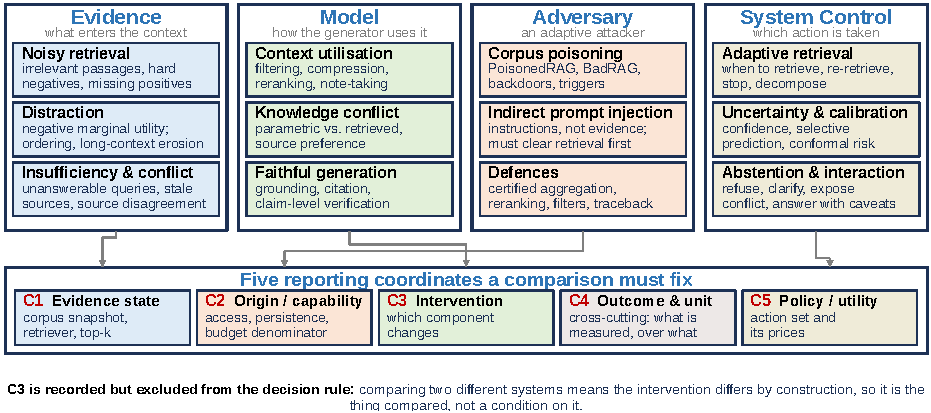
\includegraphics[width=\textwidth]{figures/generated/fig_taxonomy_map.pdf}%
\caption{The four failure surfaces and the reduction they support. Each column
is one surface of the survey (\S\ref{sec:evidence}--\S\ref{sec:system}); the
band below is the five reporting coordinates of \S\ref{sec:coordinates}, and the
connectors show which surface each coordinate collapses. C4 is cross-cutting
and has no single parent surface. The organisation is a partition of the
\emph{comparison} rather than of the literature: the columns tell a reader where
to look for related work, and the band tells a reader what must be stated on
both sides before two numbers can be placed together.}
\label{fig:hierarchical-taxonomy}
\end{figure*}

\begin{table*}[t]
\centering
\scriptsize
\renewcommand{\arraystretch}{0.88}
\begin{tabularx}{\linewidth}{>{\raggedright\arraybackslash}p{0.18\linewidth}>{\raggedright\arraybackslash}p{0.31\linewidth}>{\raggedright\arraybackslash}p{0.25\linewidth}X}
\toprule
\textbf{Boundary case} & \textbf{Rule used in this paper} & \textbf{Verdict consequence} & \textbf{Example implication} \\
\midrule
Noisy retrieval vs. distraction & Retrieval imperfection alone is coded as relevance/noise; harmful influence on generation, confidence, or reasoning is coded as distraction. & Same broad topic but different measured effect is partial. & Random negatives and hard distractors should not be pooled into one score. \\
Query/OOD vs. evidence state & Query ambiguity, distribution shift, and model uncertainty describe the need or belief state. Code them under origin unless the study labels the resulting retrieved evidence. & Shared uncertainty language does not imply a common evidence state or policy. & An OOD detector is not automatically an insufficient-context detector. \\
Natural conflict vs. adversarial corruption & Code by the source of contradiction, not by surface form. Naturally occurring or diagnostic contradiction is conflict; attacker-created contradiction is integrity/adversarial corruption. & Natural-conflict and poisoning results are invalid as a direct ranking unless the threat model is redefined. & Faithfulness or source-preference methods are not poisoning defenses by default. \\
Intervention mismatch & Code the component changed, then inspect the evaluation harness. Different interventions can be compared as alternatives if the remaining pipeline and target are controlled. & Shared harness and end-to-end target can support valid comparison; unmatched pipelines support only a qualified comparison. & A filter and a note-taking prompt can be compared after fixing retriever, generator, evidence states, budget, and action utility. \\
Metric overlap & Metric targets must match the object being measured. Accuracy, citation support, attack success, calibration, and selective risk are separate families. & Shared dataset but different metric family is partial; mutually incompatible targets are invalid for one-scalar ranking. & A correct answer with unsupported citation should not pass a faithfulness comparison. \\
Observable but unnamed action & Infer behavior only when action is decision-relevant and the protocol is unambiguous; otherwise use \emph{not applicable}. & Merely omitting the phrase ``action policy'' does not force under-specification. & An answer-only benchmark supplies \emph{answer} for a policy claim, but a fixed latency comparison needs no action label. \\
Security capability missing & Mark only decision-critical missing access, budget, objective, or target as unknown. A shared harness may intentionally vary capability. & Unknown capability makes a cross-game rank under-specified; controlled capability variation can support a valid descriptive contrast. & Black- and white-box variants of one attack can be compared inside the same harness without implying cross-paper transfer. \\
Benchmark vs. method & Code benchmark if the reusable artifact is the main contribution; otherwise code the intervention. & Benchmark-method comparison is partial unless the method is evaluated on the benchmark under aligned assumptions. & RGB is benchmark-first; RAAT is training-first. \\
Tuple match but control mismatch & After semantic coding, inspect corpus, data, retriever, generator, top-$k$, budget, baselines, decoding, and uncertainty. & A tuple match is insufficient for direct ranking when these factors confound the reported score. & Two answer-only noise methods on different datasets and generators require a shared rerun or a qualified claim. \\
\bottomrule
\end{tabularx}
\caption{Boundary rules for applying the revised diagnostic schema. Verdicts are claim-specific and require both semantic and experimental-control checks.}
\label{tab:taxonomy-rules}
\end{table*}

\begin{figure*}[t]
\centering
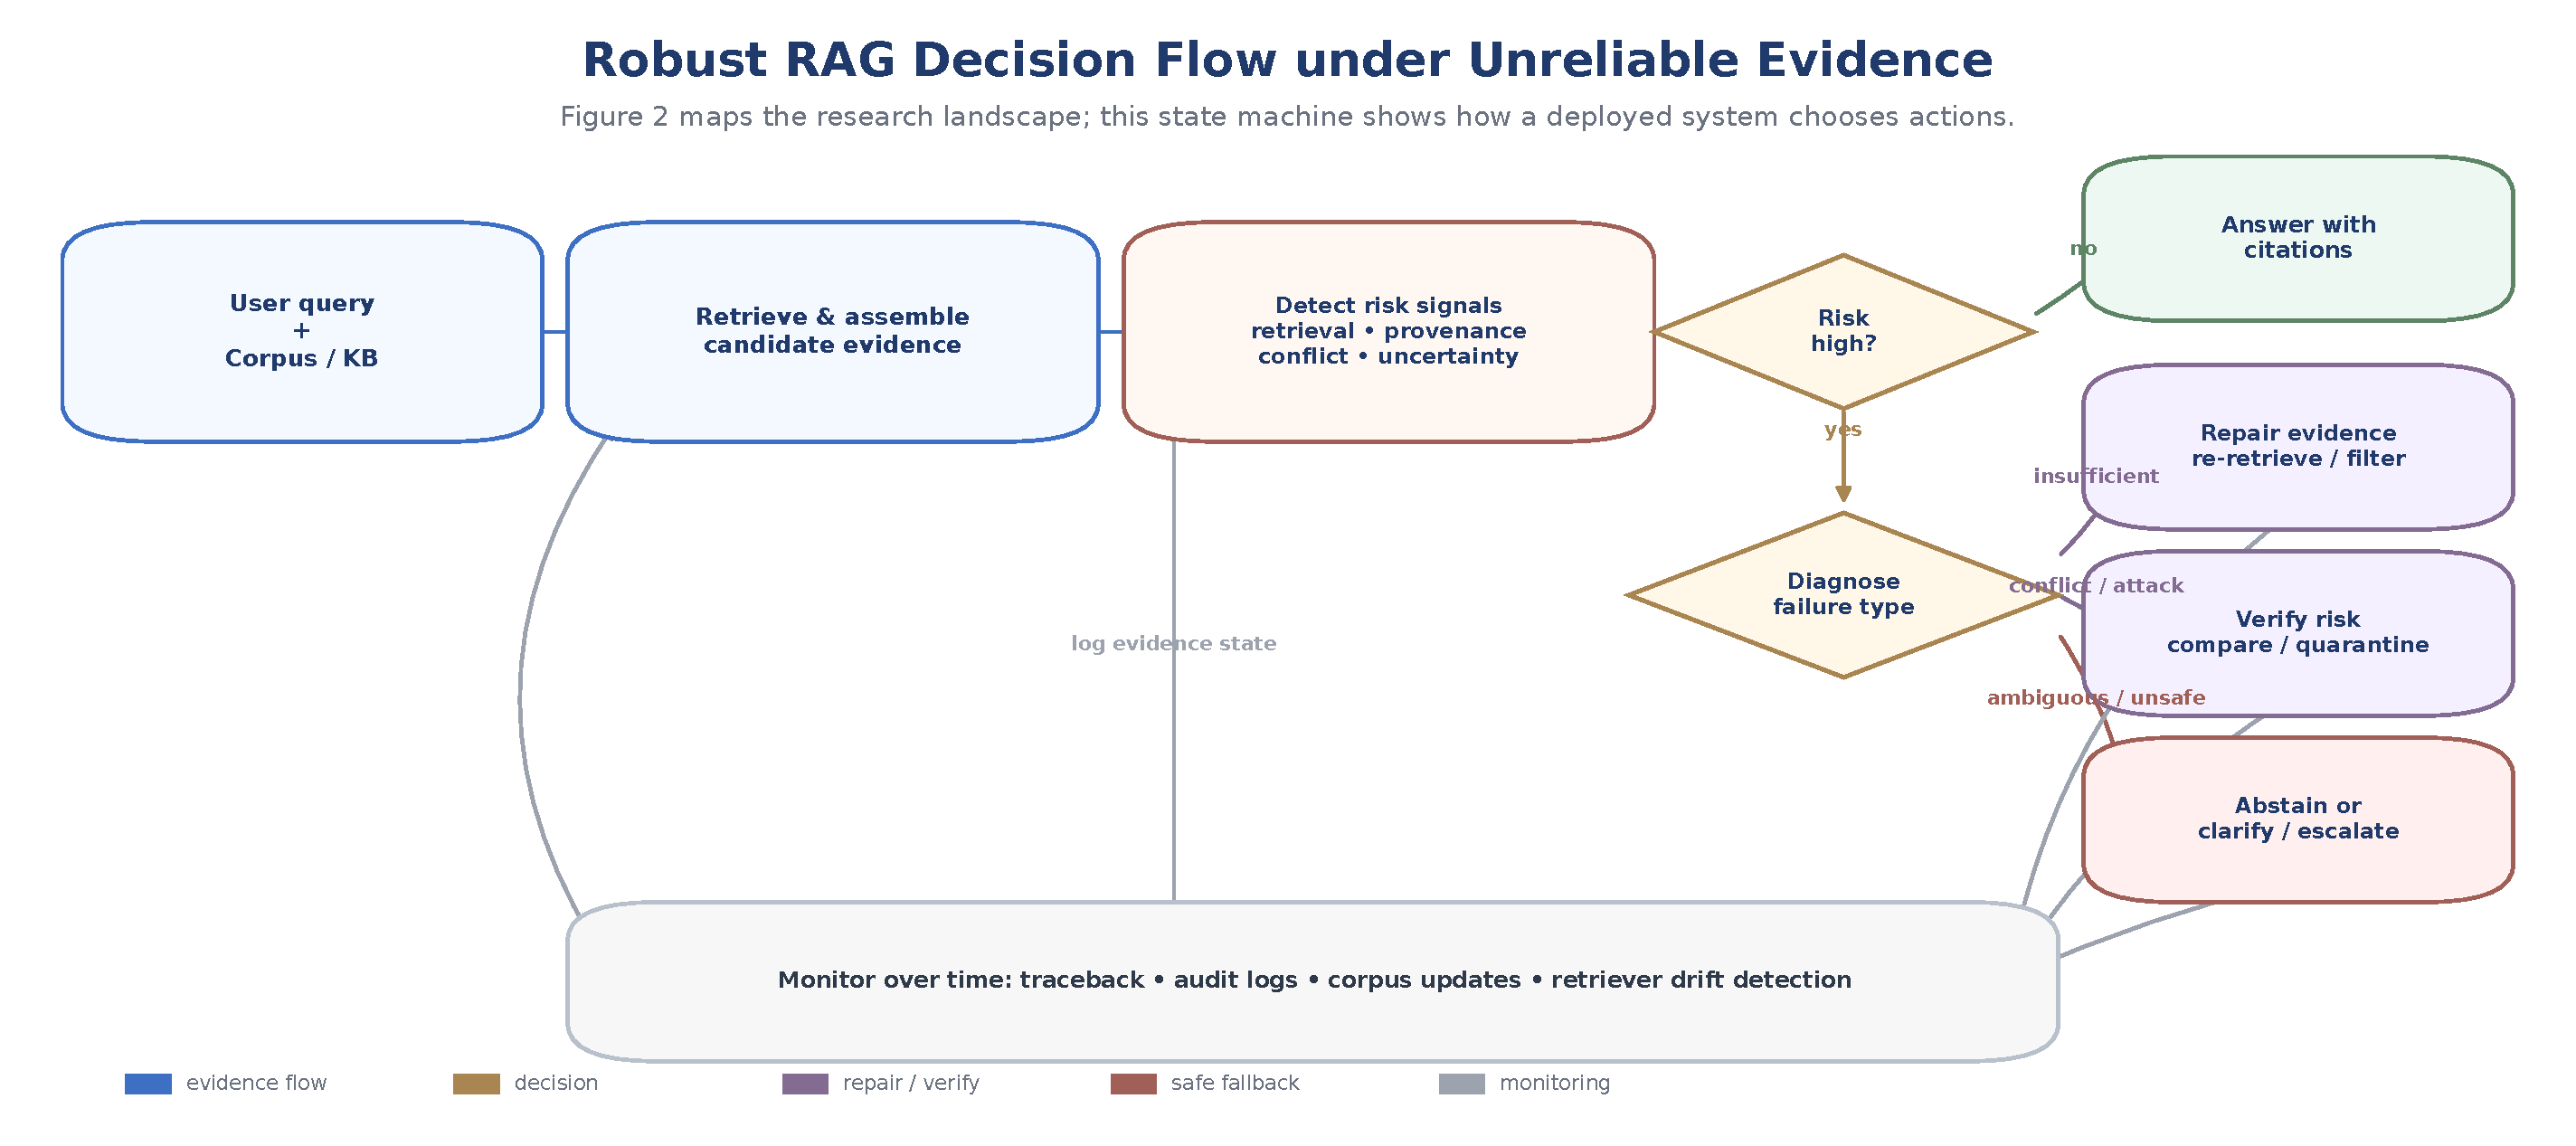
\includegraphics[width=\textwidth,keepaspectratio]{figures/generated/fig3_operational_decision_flow_py_4k.pdf}
\caption{Operational decision flow for robust RAG. Unlike the taxonomy in Figure~\ref{fig:hierarchical-taxonomy}, this state-machine view describes the branching actions a deployed system can take when unreliable evidence is encountered: answer, repair evidence, verify risk, abstain, clarify, escalate, or monitor.}
\label{fig:operational-pipeline-image}
\end{figure*}

\begin{table*}[t]
\centering
\small
\begin{tabularx}{\linewidth}{p{0.14\linewidth}p{0.2\linewidth}p{0.27\linewidth}X}
\toprule
\textbf{Stage} & \textbf{Question} & \textbf{Typical signals} & \textbf{Representative actions} \\
\midrule
Detect & Is the current evidence unreliable? & Low retrieval confidence, high contradiction, low sufficient-context score, suspicious document patterns & Flag query/evidence, route to stronger checks, log risk state \\
Diagnose & What kind of unreliability is present? & Irrelevance, distraction, conflict, poisoning, ambiguity, unanswerability, stale evidence & Assign failure type; separate benign noise from adversarial risk \\
Mitigate & Can the evidence be repaired before answering? & Alternative retrieval results, filter scores, reranker utility, provenance, source agreement & Re-rank, filter, compress, re-query, retrieve from trusted sources, remove malicious passages \\
Control & What should the system do now? & Calibrated confidence, selective risk, cost budget, user risk tolerance & Answer, abstain, ask clarification, expose conflict, escalate to human review \\
Monitor & Did the system fail or get attacked? & User feedback, traceback signals, poisoned-document clusters, drift over time & Update index, quarantine sources, revise prompts, retrain filters, update audit logs \\
\bottomrule
\end{tabularx}
\caption{An operational pipeline for robust RAG. The pipeline turns the paper's taxonomy into actionable system design steps.}
\label{tab:operational-pipeline}
\end{table*}


\part*{Part II: Testing and Applying the Taxonomy}
\label{app:part-audit}

\FloatBarrier
\section{Comparability Case Ledger}
\label{sec:appendix-cases}
\label{sec:cases}
\begin{table*}[t]
\centering\scriptsize
\setlength{\tabcolsep}{2pt}
\begin{tabular}{@{}>{\raggedright\arraybackslash}p{0.048\textwidth}>{\raggedright\arraybackslash}p{0.050\textwidth}>{\raggedright\arraybackslash}p{0.140\textwidth}>{\raggedright\arraybackslash}p{0.098\textwidth}>{\raggedright\arraybackslash}p{0.062\textwidth}>{\raggedright\arraybackslash}p{0.062\textwidth}>{\raggedright\arraybackslash}p{0.390\textwidth}@{}}
\toprule
ID & Src & Compared results & Quoted gap & Mismatch & Verdict & Consequence of matching the coordinate \\
\midrule
SEC-01 & rerun & PoisonedRAG vs.~CorpusPoisoning & 1\% vs 84.2\% for the same attack & C1, C2, C4 & undefined & C4 differs: 0.01 scores answer manipulation, 84.2 scores top-20 retrieval, so no gap is defined. \\
SEC-02 & invited & PoisonedRAG vs.~Phantom & +3.7\% ASR in favor of PoisonedRAG & C1, C2, C4 & undefined & No matched operating point exists for C4 (targeted answer vs refusal), so no gap is defined at any budget. \\
SEC-03 & no num. & RobustRAG vs.~PoisonedRAG & Defense credited with reducing poisoning ASR to <=15\% & C1, C2, C4 & undefined & No number is transported; RobustRAG re-implements the attack, and its own poisoning ASRs are 37-86. \\
SEC-04 & quoted & BadRAG vs.~PoisonedRAG & +1.2\% in favor of BadRAG (98.2\% vs 97\%) & C2, C4, C5 & undefined & Objectives differ (denial of service vs targeted answer), so the 1.2-point gap does not rank the two attacks. \\
SEC-05 & rerun & AIP vs.~PoisonedRAG & +66.66\% ASR in favor of AIP & C1, C2 & narrows & At five injected documents on MedSquad the 66.66-point gap stands; it does not transfer to NQ. \\
NOISE-01 & rerun & CRAG (Self-CRAG) vs.~Self-RAG 7B & +6.9 accuracy in favor of Self-CRAG & C3 & survives & All five coordinates match, so the 6.9-point gap stands as reported. \\
NOISE-02 & rerun & CtrlA 7B vs.~Self-RAG 7B & +6.9 accuracy in favor of CtrlA & C1, C3 & narrows & Backbone and retriever differ, so the 6.9-point gap has no determined sign. \\
NOISE-03 & invited & RGB (ChatGPT) vs.~RAAT (ChatGPT3.5) & +4.53 accuracy/EM in favor of RGB's ChatGPT & C1, C4 & undefined & Substring accuracy is weaker than exact match, so the 4.53-point gap has no determined sign. \\
NOISE-04 & invited & Chain-of-Note vs.~RAAT (ChatGPT3.5) & +7.55 vs +1.68 EM gain & C1, C3, C4 & undefined & The two baselines differ in whether gold context is present, so the two gains are not commensurable. \\
NOISE-05 & rerun & AstuteRAG vs.~RobustRAG & +4.4 accuracy in favor of ASTUTE RAG & C1, C5 & survives & Model, dataset, retrieval and metric match, so the 4.4-point accuracy gap stands. \\
FAITH-02 & quoted & FaithfulRAG vs.~FaithEval (GPT-4o CF) & 81.7\% vs 47.5\% (+34.2) & C1, C4 & undefined & Aggregate and single-task scores under different conflict types and models cannot be differenced. \\
CALIB-03 & invited & ADAPT-LLM vs.~Self-RAG 7B & +16.75 accuracy in favor of Self-RAG & C1, C4 & narrows & A harder test subset and a stricter metric are confounded with the method, so 16.75 is not a method effect. \\
\midrule
\multicolumn{7}{@{}l}{\emph{Within-harness controls (one paper, one harness)}} \\
FAITH-01 & invited & RAGTruth (resp-level) vs.~RAGTruth (span-level) & 78.7\% F1 vs span-level & C4 & narrows & Response-level and span-level scores are different units, so the contrast holds only within one unit. \\
CALIB-01 & stated & Self-RAG 7B vs.~RAG-baseline & +23.9 accuracy in favor of Self-RAG & C3 & survives & Within one paper and one harness the 23.9-point gap stands as reported. \\
CALIB-02 & stated & CtrlA 7B vs.~FLARE (reimpl.) & +4.0 accuracy in favor of CtrlA & C3 & survives & Within one paper and one harness the 4.0-point gap stands as reported. \\
\bottomrule
\end{tabular}
\caption{Worked cross-paper comparisons. Of 12 comparisons published papers state (Src=stated) or invite by grouping (Src=invited), 7 have no common scope, 3 survive only on a strict subset and 2 survive as stated; 3 within-harness contrasts are negative controls. \emph{Src} also records how the other side's number reached the citing paper: \emph{quoted} transports it, \emph{rerun} re-implements the other system in this harness, \emph{no num.} asserts a relation without giving the other side's number, and \emph{invited} is a juxtaposition no author stated. Every number is copied verbatim from a locally extracted full text and re-checked at its line by \texttt{verify\_cross\_paper\_cases.py}; all \VerifChecks{} provenance, numeral and verbatim-quotation checks pass. C1 evidence state, C2 origin/capability, C3 intervention, C4 outcome, C5 policy/utility; the rule of \S\ref{sec:estimands} is applied exactly, so only C1, C2, C4 and C5 threaten a comparison and a C3 mismatch never does. An independent \RecJudges{}-judge panel reproduces these verdicts on \RecBinaryPct\% of the cross-paper rows for the binary distinction the paper uses and \RecThreeWayPct\% for the three-way label (Table~\ref{tab:ledger-recoding}), which is why no rate from this table is quoted as a result. The per-case source line ranges, the full side-A and side-B reported values and the coordinate-matched readings are released as \texttt{supplement/cross\_paper\_comparability\_cases.csv}.}
\label{tab:cross-paper-cases}
\end{table*}

\begin{table}[t]
\centering\scriptsize
\setlength{\tabcolsep}{3pt}
\begin{tabular}{@{}lllll@{}}
\toprule
Case & Kind & Ours & Independent panel & Agree \\
\midrule
CALIB-03 & cross & narrows & unde~6 & 0/6 \\
FAITH-02 & cross & undefined & surv~3, unde~3 & 3/6 \\
NOISE-01 & cross & survives & surv~6 & 6/6 \\
NOISE-02 & cross & narrows & unde~6 & 0/6 \\
NOISE-03 & cross & undefined & unde~6 & 6/6 \\
NOISE-04 & cross & undefined & unde~6 & 6/6 \\
NOISE-05 & cross & survives & surv~4, unde~2 & 4/6 \\
SEC-01 & cross & undefined & unde~5, surv~1 & 5/6 \\
SEC-02 & cross & undefined & unde~5, narr~1 & 5/6 \\
SEC-03 & cross & undefined & narr~5, unde~1 & 1/6 \\
SEC-04 & cross & undefined & unde~6 & 6/6 \\
SEC-05 & cross & narrows & unde~3, surv~3 & 0/6 \\
CALIB-01 & ctrl & survives & surv~3, unde~3 & 3/6 \\
CALIB-02 & ctrl & survives & surv~6 & 6/6 \\
FAITH-01 & ctrl & narrows & unde~6 & 0/6 \\
\bottomrule
\end{tabular}
\caption{The ledger holds up on the distinction it is used for and not on the three-way label. Six judges from three developers re-code every case from the neutral statement of the juxtaposition and the verbatim source excerpts alone, never seeing our coordinate labels, our reading, our matched number or our verdict. On the 12 cross-paper cases the panel majority reproduces our three-way verdict on 58\% of cases ($\kappa=0.32$), and agreement among the six judges themselves is $\kappa=0.52$. On the binary distinction the paper's conclusion actually uses---does the quoted gap stand as reported---the majority reproduces us on 100\% and the panel is unanimous on 67\% of cases. This is why we report the ledger's negative statements and not a rate.}
\label{tab:ledger-recoding}
\end{table}


\FloatBarrier
\section{Screening Frame, Census and Codebook Ablation}
\label{sec:appendix-census}
% Drawn by scripts/revision3/fig_appendix_flows.py; the .pptx is the editable
% source and is released with the paper.
\begin{figure}[t]
\centering
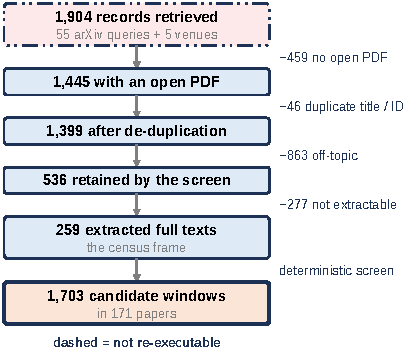
\includegraphics[width=\columnwidth]{figures/generated/fig_screening_flow.pdf}%
\caption{Sampling frame for the census. Solid boxes are stages a third party
can re-execute from the release; the dashed box is documented but not
re-executable, because per-query hit counts were not logged at the snapshot
date and live indices drift. The frame is therefore reconstructible from the
259 released texts downward, and the population those texts were drawn from is
not. Every composition figure in this paper is stated for the frame or for the
re-weighted window universe, never for the literature.}
\label{fig:screening-frame-flow}
\end{figure}

% Generated by scripts/revision4/analyze_frame_coverage.py -- do not edit.
\begin{table}[t]
\centering\scriptsize
\setlength{\tabcolsep}{3pt}
\resizebox{\columnwidth}{!}{%
\begin{tabular}{@{}lrrrrrr@{}}
\toprule
Prior survey & Refs & In-sc. & Ded. & Scr. & Text & Map \\
\midrule
RAG survey (Gao) \citep{ragSurvey2024} & 227 & 8 & 0.50 & 0.38 & 0.25 & 0.62 \\
RAG evaluation (Yu) \citep{ragEvaluationSurvey2024} & 74 & 2 & 0.00 & 0.00 & 0.00 & 0.50 \\
Trustworthy RAG (Zhou) \citep{trustRAGCompass2024} & 192 & 28 & 0.64 & 0.50 & 0.46 & 0.50 \\
Securing RAG (Xu) \citep{securityRAGSurvey2026} & 121 & 69 & 0.75 & 0.64 & 0.55 & 0.58 \\
Knowledge conflicts (Xu) \citep{xuKnowledgeConflicts2024} & 200 & 3 & 0.33 & 0.33 & 0.33 & 0.33 \\
Abstention (Wen) \citep{wenAbstentionSurvey2025} & 179 & 1 & 0.00 & 0.00 & 0.00 & 0.00 \\
\midrule
\textbf{Pooled} & 878 & 95 & 0.67 & 0.56 & 0.47 & 0.54 \\
\midrule
\multicolumn{7}{@{}l}{\emph{Pooled in-scope recall, Wilson 95\% CI}} \\
Deduped (1,399) & \multicolumn{6}{r}{0.67 [0.57, 0.76] (64/95)} \\
Full texts (259) & \multicolumn{6}{r}{0.47 [0.38, 0.57] (45/95)} \\
\bottomrule
\end{tabular}}
\caption{Coverage of the six prior surveys' reference lists against our frame, the reviewer's requested recall-against-a-known-list check. \emph{Refs} is the bibliography Semantic Scholar resolves for each survey; \emph{In-sc.}\ keeps titles naming both a retrieval and a robustness concept (keyword lists released in \texttt{frame\_coverage\_audit.json}). The stage columns give the share of in-scope references present in the deduplicated release (1,399), the relevance-screened set (536), the extracted full texts (259) and the adjudicated Map~B (342); matching is by arXiv id, DOI, ACL id, then normalised title. The 1,904 retrieved and 1,445 open-PDF stages are count-only in the release, so the deduplicated column lower-bounds retrieval recall. Per-survey CIs and unfiltered recall are in the released JSON.}
\label{tab:frame-coverage}
\end{table}

% Generated by scripts/revision3/build_revision3_tables.py -- do not edit.
\begin{table*}[t]
\centering\scriptsize
\setlength{\tabcolsep}{3pt}
\begin{tabular}{@{}lrrrcrr@{}}
\toprule
Judgment & Ref.\ est. & Scored & Acc. & 95\% CI & Base & Acc.\ (LOO) \\
\midrule
Provenance (transported / re-implemented / unclear) & 171 & 170 & 0.91 & [0.86, 0.96] & 0.79 & 0.89 \\
Verdict (survives / narrows / undefined) & 129 & 114 & 0.82 & [0.74, 0.89] & 0.77 & 0.81 \\
\midrule
\multicolumn{7}{@{}l}{\emph{Per-class recall of the deployed panel, provenance}} \\
\quad transported & & 35 & 0.80 & [0.64, 0.90] & & \\
\quad re-implemented & & 135 & 0.93 & [0.88, 0.96] & & \\
\quad unclear & & 0 & -- & -- & & \\
\bottomrule
\end{tabular}
\caption{The deployed panel scored on \emph{real} frame windows against a
privileged-information reference, whose adjudicators read both papers' full
texts rather than a 45-line window and whose every counted vote carries a quote
located mechanically in the document that adjudicator was shown. ``Ref.\ est.''
counts windows with a quote-verified majority; those without one are reported,
not dropped. ``Base'' is the majority-class rate. The last column removes the one
adjudicator sharing a checkpoint with the deployed panel. Measured sensitivity
1.00 and specificity 0.99 for the transported class make the composition
correction non-trivial, unlike the identity map the submitted version used: it
moves the re-implemented share to 0.881. This is not human gold.}
\label{tab:privileged-reference}
\end{table*}

% Generated by scripts/revision4/build_revision4_tables.py -- do not edit.
\begin{table}[t]
\centering\scriptsize
\setlength{\tabcolsep}{4pt}
\begin{tabular}{@{}lrrr@{}}
\toprule
\multicolumn{4}{@{}l}{\emph{Worst-/best-case accuracy folding in excluded windows}} \\
Setting & $N$ & Worst & Best \\
\midrule
Verdict: scored (93/114) & 114 & 0.82 & 0.82 \\
\quad over full sample & 180 & 0.52 & 0.88 \\
\quad over deployed-committed & 159 & 0.58 & 0.87 \\
\quad reviewer $114{+}51$ & 165 & 0.56 & 0.87 \\
Provenance: scored (154/170) & 170 & 0.91 & 0.91 \\
\quad over full sample & 180 & 0.86 & 0.91 \\
\quad over deployed-committed & 179 & 0.86 & 0.91 \\
\midrule
\multicolumn{4}{@{}l}{\emph{No-majority (51) vs.\ established (129) verdict windows}} \\
Feature & Estab. & No-maj. & Test \\
\midrule
Quote-verified ref.\ votes (med.) & 3 & 1 & $p{<}0.001$, $\delta{=}+0.79$ \\
Ref.\ vote-split entropy (mean) & 0.53 & 0.88 & $p{<}0.001$, $\delta{=}-0.38$ \\
Survey-table stratum (share) & 0.28 & 0.51 & $p{=}0.007$, $V{=}0.23$ \\
Deployed panel commits (rate) & 0.88 & 0.88 & $p{=}1.00$, $V{\approx}0$ \\
Window length (med.\ words) & 85 & 70 & $p{=}0.32$, $\delta{=}-0.09$ \\
Coordinate terms (median) & 2 & 3 & $p{=}0.13$, $\delta{=}-0.14$ \\
\bottomrule
\end{tabular}
\caption{Reviewer Q6: bounds and characterisation for the excluded privileged-reference windows. \emph{Top:} the deployed panel is scored only where the reference reached a quote-verified majority (verdict 93/114$=\,$0.82, Wilson [0.73, 0.88]; provenance 154/170$=\,$0.91, [0.85, 0.94]). Worst case counts the panel wrong on every folded-in window, best case right. The reviewer's $114{+}51{=}165$ denominator overstates the panel's committed set: only 45 of the 51 no-reference-majority windows carry a deployed verdict, so the deployed-committed total is 159, not 165. \emph{Bottom:} the no-majority windows differ from the rest mainly in having fewer quote-verified privileged votes and more split ones, and in stratum mix; they are not longer, denser in coordinate terms, or harder for the deployed panel, which commits on them at the same rate. Continuous features: Mann--Whitney $p$ and Cliff's $\delta$; categorical: $\chi^2$ $p$ and Cram\'er's $V$ (deployed-commits uses Fisher).}
\label{tab:privileged-reference-bounds}
\end{table}

% Generated by scripts/revision3/build_revision3_tables.py -- do not edit.
\begin{table}[t]
\centering\scriptsize
\setlength{\tabcolsep}{3pt}
\resizebox{\columnwidth}{!}{%
\begin{tabular}{@{}lrrrr@{}}
\toprule
\multicolumn{5}{@{}l}{\emph{Did the panel execute its own rule?}} \\
& $n$ & $\kappa$ & 95\% CI & \\
Verdict as \emph{stated} by the judges & 704 & 0.06 & [-0.01, 0.11] & \\
Verdict \emph{composed} from their own coordinates & 704 & 0.09 & [0.01, 0.15] & \\
$\Delta$ (composed $-$ stated) & & +0.02 & [0.00, 0.05] & \\
\midrule
\multicolumn{5}{@{}l}{\emph{Rule fidelity, judge by judge: share of codings where stated $=$ composed, and}} \\
\multicolumn{5}{@{}l}{\emph{count of \textbf{survives} verdicts the judge's own coordinates contradict}} \\
\quad coderA\_gpt5mini & \multicolumn{2}{r}{1.000} & \multicolumn{2}{r}{0} \\
\quad coderB\_claudeopus46 & \multicolumn{2}{r}{0.770} & \multicolumn{2}{r}{162} \\
\quad coderC\_gemini31pro & \multicolumn{2}{r}{0.925} & \multicolumn{2}{r}{53} \\
\midrule
\multicolumn{5}{@{}l}{\emph{What the evidence quotes are: 1,879 non-empty quotes classified}} \\
\quad verbatim in the passage shown & \multicolumn{2}{r}{1,639} & \multicolumn{2}{r}{0.872} \\
\quad verbatim after Unicode/de-hyphenation & \multicolumn{2}{r}{80} & \multicolumn{2}{r}{0.043} \\
\quad abridged with an ellipsis, fragments verbatim & \multicolumn{2}{r}{76} & \multicolumn{2}{r}{0.040} \\
\quad table re-serialised from the passage & \multicolumn{2}{r}{59} & \multicolumn{2}{r}{0.031} \\
\quad elsewhere in the same paper & \multicolumn{2}{r}{--} & \multicolumn{2}{r}{0.000} \\
\quad re-serialised from elsewhere & \multicolumn{2}{r}{4} & \multicolumn{2}{r}{0.002} \\
\quad near paraphrase of the passage & \multicolumn{2}{r}{--} & \multicolumn{2}{r}{0.000} \\
\quad absent from the source document & \multicolumn{2}{r}{21} & \multicolumn{2}{r}{0.011} \\
\bottomrule
\end{tabular}}
\caption{Two diagnostics the submitted version did not run, both over data it
had already released. \emph{Top:} the decision rule of \S\ref{sec:estimands}
composed mechanically from each judge's own coordinate labels, beside the
verdict that judge stated. Composing the rule does not make the panel
reproducible, so the census failure is not the panel failing to execute its
instrument. \emph{Bottom:} every evidence quote classified against the passage
its author was shown. The submitted version reported a single located rate,
which pools an extraction artefact with a fabrication; separating them shows
0.987 of non-empty quotes are
supported by the passage shown and
0.011 are absent from the source
document altogether.}
\label{tab:census-diagnostics}
\end{table}

% Generated by scripts/revision3/build_revision3_tables.py -- do not edit.
\begin{table}[t]
\centering\scriptsize
\setlength{\tabcolsep}{3pt}
\resizebox{\columnwidth}{!}{%
\begin{tabular}{@{}lrrrrr@{}}
\toprule
Field & Maj.\ share & Obs. & $\kappa$ & $\kappa_{\max}$ & $\kappa/\kappa_{\max}$ \\
\midrule
C1 evidence state & 0.630 & 0.60 & +0.19 & 0.72 & 0.26 \\
C2 origin / capability & 0.589 & 0.54 & +0.11 & 0.61 & 0.18 \\
C3 intervention & 0.871 & 0.75 & -0.11 & 0.42 & -0.26 \\
C4 outcome / unit & 0.814 & 0.71 & +0.08 & 0.53 & 0.16 \\
C5 policy / utility & 0.526 & 0.54 & +0.10 & 0.51 & 0.19 \\
Verdict & 0.507 & 0.45 & +0.06 & 0.46 & 0.13 \\
\midrule
\multicolumn{6}{@{}l}{\emph{The headline contrast, on matched label spaces}} \\
Census, three classes & & 0.45 & 0.06 & 0.46 & 0.13 \\
Census, binary & & 0.52 & 0.05 & 0.37 & 0.12 \\
Constructed (stated), three classes & & 0.83 & 0.74 & 0.81 & 0.92 \\
Constructed (stated), binary & & 0.95 & 0.86 & 0.88 & 0.97 \\
\bottomrule
\end{tabular}}
\caption{How much room $\kappa$ had. $\kappa_{\max}$ is Cohen's maximum
attainable $\kappa$, averaged over judge pairs: the largest value these judges
could have reached without changing how often each of them uses each label
\citep{umesh1989maxkappa,sim2005kappa}. A near-constant field caps $\kappa$
regardless of behaviour, which is the argument \S\ref{sec:estimands} makes for
C3; the last column applies it to every field instead of one, so the argument is
symmetric. It also repairs the headline contrast: matching the label space does
not close the gap between the constructed and the published setting, and the
right reading of the census verdict is that its judges reach
0.13 of what their own marginals allow
where the constructed judges reach 0.92.}
\label{tab:kappa-ceiling}
\end{table}

% Generated by scripts/revision3/build_revision3_tables.py -- do not edit.
\begin{table}[t]
\centering\scriptsize
\setlength{\tabcolsep}{3pt}
\begin{tabular}{@{}lrrrrc@{}}
\toprule
Passage discloses \dots & Windows & Papers & Obs. & $\kappa$ & 95\% CI \\
\midrule
\quad 0 of four disclosed & 44 & 9 & 0.66 & 0.10 & [-0.14, 0.33] \\
\quad 1 of four disclosed & 23 & 9 & 0.42 & -0.11 & [-0.32, 0.09] \\
\quad 2 of four disclosed & 157 & 25 & 0.44 & 0.04 & [-0.13, 0.09] \\
\quad 3 of four disclosed & 253 & 60 & 0.42 & -0.02 & [-0.13, 0.05] \\
\quad 4 of four disclosed & 227 & 57 & 0.44 & 0.08 & [-0.07, 0.18] \\
\midrule
High ($\geq 3$) & 480 & & & 0.03 & \\
Low ($\leq 2$) & 224 & & & 0.11 & \\
Difference (high $-$ low) & & & & -0.08 & [-0.27, 0.05] \\
\bottomrule
\end{tabular}
\caption{The disclosure counterfactual on published text. Disclosure is scored
deterministically from a released lexicon over the passage the judges were
shown, so the exposure is a document feature and not a model output: regressing
agreement on it is not regressing the panel's labels on themselves. Windows
whose passages mention more coordinate-relevant terms do \emph{not} yield more
reproducible verdicts. This is the observational test of the checklist
recommendation, and it does not support it; \S\ref{sec:instrument} shows what
does, and what does not follow from it.}
\label{tab:disclosure-counterfactual}
\end{table}

\begin{table}[t]
\centering\scriptsize
\setlength{\tabcolsep}{3pt}
\begin{tabular}{@{}lrrrrr@{}}
\toprule
Panel & $J$ & \multicolumn{2}{c}{Common items} & All & Own \\
\cmidrule(lr){3-4}\cmidrule(lr){5-5}\cmidrule(lr){6-6}
 & & $AC_1$ & $\kappa$ & $\kappa$ & $\kappa$ \\
\midrule
Submitted panel (1 mini, 2 front.) & 3 & 0.29 & 0.14 & 0.33 & 0.07 \\
Small tier only, 3 developers & 3 & 0.16 & 0.00 & 0.29 & 0.00 \\
Frontier only, 3 developers & 3 & 0.54 & 0.31 & 0.51 & 0.25 \\
Frontier only, 3 dev.\ $\times$ 2 checkpoints & 6 & 0.47 & 0.22 & 0.38 & 0.23 \\
\quad same dev.\ (Anthropic) & 2 & 0.56 & 0.35 & 0.51 & 0.49 \\
\quad same dev.\ (Google) & 2 & 0.54 & 0.29 & 0.38 & 0.24 \\
\quad same dev.\ (OpenAI) & 2 & 0.53 & 0.20 & 0.50 & 0.21 \\
\quad across dev.\ (pair A) & 2 & 0.56 & 0.32 & 0.53 & 0.37 \\
\quad across dev.\ (pair B) & 2 & 0.37 & 0.07 & 0.15 & 0.24 \\
\bottomrule
\end{tabular}
\caption{Upgrading the judges helps and does not rescue the verdict, on a population that is identical for every row. The same \FrameCandidates{}-window frame is coded by a fully crossed pool of nine judges---a small and two frontier checkpoints from each of three developers---from which these panels are drawn. Because $\kappa$ is prevalence sensitive, comparing panels each scored on its own majority-eligible subset would confound capability with item composition, so \emph{Common items} fixes one population of 843 windows that a majority of the whole nine-judge pool called eligible, and \emph{All} drops nothing at all: it scores every one of the 1,680 commonly coded windows, carrying ineligibility as its own category. \emph{Own} is each panel's $\kappa$ recomputed on the majority-eligible subset of \emph{that panel}, which is the population a reader who ran only that panel would see; it is reported because it is what a smaller pool can obtain, and it is the column that must \emph{not} be compared across rows. Conclusions are unchanged across the three: an all-frontier panel of three developers multiplies verdict $\kappa$ several-fold over the submitted panel and still reaches only \emph{fair}. The three \emph{same dev.} rows are the reference level, two frontier checkpoints from one developer where nothing differs but the checkpoint; they bound what \emph{correlated} judges reach, not what the task affords, and Table~\ref{tab:frontier-pairs} shows that one cross-developer pair beats two of them.}
\label{tab:tier-control}
\end{table}

\begin{table}[t]
\centering\scriptsize
\setlength{\tabcolsep}{4pt}
\begin{tabular}{@{}llrrr@{}}
\toprule
Frontier pair & Dev. & $\kappa$ & $AC_1$ & Elig.\ $\kappa$ \\
\midrule
opus-4.6 vs opus-4.8 & same & 0.35 & 0.56 & 0.56 \\
opus-4.6 vs gem-3.1p & cross & 0.32 & 0.56 & 0.61 \\
gem-3.1p vs gpt-5.4 & cross & 0.32 & 0.53 & 0.67 \\
gem-3.1p vs gem-2.5p & same & 0.29 & 0.54 & 0.50 \\
opus-4.6 vs gpt-5.4 & cross & 0.29 & 0.52 & 0.61 \\
opus-4.8 vs gpt-5.4 & cross & 0.25 & 0.50 & 0.43 \\
gem-2.5p vs gpt-5.4 & cross & 0.22 & 0.47 & 0.52 \\
opus-4.6 vs gem-2.5p & cross & 0.20 & 0.47 & 0.33 \\
gpt-5.4 vs gpt-5.5 & same & 0.20 & 0.53 & 0.71 \\
gem-3.1p vs opus-4.8 & cross & 0.19 & 0.44 & 0.43 \\
opus-4.8 vs gpt-5.5 & cross & 0.11 & 0.50 & 0.26 \\
opus-4.8 vs gem-2.5p & cross & 0.07 & 0.37 & 0.16 \\
gem-2.5p vs gpt-5.5 & cross & 0.07 & 0.42 & 0.64 \\
gem-3.1p vs gpt-5.5 & cross & 0.03 & 0.34 & 0.63 \\
opus-4.6 vs gpt-5.5 & cross & 0.00 & 0.35 & 0.49 \\
\bottomrule
\end{tabular}
\caption{Every frontier-frontier judge pair, on the common item population, ordered by verdict $\kappa$. The averaged same-developer advantage is +0.11; its exact randomisation over the 15 ways of matching six checkpoints into three disjoint pairs gives $p=0.07$, against a smallest attainable value of 0.07. The contrast is also not uniform: 6 cross-developer pairs agree better than the weakest same-developer pair, so sharing a developer is reported as residual structure and not as an effect.}
\label{tab:frontier-pairs}
\end{table}

\begin{table*}[t]
\centering\scriptsize
\setlength{\tabcolsep}{3pt}
\begin{tabular}{@{}lrrrrl@{}}
\toprule
Instrument & $AC_1$ & $\kappa$ & Unan. & \emph{Survives} share & $\Delta\kappa$ \\
\midrule
Five coordinates (released) & 0.54 & 0.31 & 0.48 & 0.40--0.63 & --- \\
C1 and C4 only & 0.56 & 0.34 & 0.51 & 0.55--0.62 & +0.03 [-0.05, +0.12] \\
No coordinates, asked directly & 0.58 & 0.31 & 0.53 & 0.62--0.73 & -0.00 [-0.10, +0.11] \\
\bottomrule
\end{tabular}
\caption{The verdict does not become reliable when the instrument is simplified. The same three frontier judges, one per developer, code the same \FrameCandidates{}-window frame three times, changing only the codebook: the released five coordinates, the two coordinates that are not degenerate across systems, and no coordinates at all. All three arms are scored on the same 832 windows. $\Delta\kappa$ is against the five-coordinate arm with a 95\% interval resampling source papers. \emph{Survives} share is the range across the three judges of how often each calls a comparison sound; the spread, not the noise, is what fails to port.}
\label{tab:codebook-ablation}
\end{table*}

\begin{table}[t]
\centering\scriptsize
\setlength{\tabcolsep}{3pt}
\begin{tabular}{@{}lrrr@{}}
\toprule
Subset & $N$ & Accuracy & 95\% CI \\
\midrule
Panel majority, all items & 238 & 0.945 & [0.92, 0.97] \\
\quad passage declares provenance & 79 & 1.000 & [1.00, 1.00] \\
\quad provenance only from structure & 80 & 1.000 & [1.00, 1.00] \\
\midrule
\quad recall, reimplemented & 80 & 1.000 & [1.00, 1.00] \\
\quad recall, transported & 79 & 1.000 & [1.00, 1.00] \\
\quad recall, unclear & 79 & 0.835 & [0.75, 0.91] \\
\midrule
Constant baseline & 238 & 0.336 & --- \\
\bottomrule
\end{tabular}
\caption{The provenance label scored against a reference, not against agreement. Items are constructed excerpts whose provenance is fixed when the item is written; the prompt, the three judges and the majority rule are byte-identical to the ones that produced the census labels. The three reference classes are equinumerous, so the constant baseline is $1/3$. The \emph{implicit} rows carry no declaration sentence at all, so a classifier that keyed on a re-implementation or attribution phrase would score at baseline there. The stratum that asserts a relation while supplying no number for the other side is not scorable under a three-option prompt and is reported separately: the deployed prompt sends 100\% of those judgments to \emph{unclear}, while the same prompt with a fourth option recovers them at 100\%, so the category is codable and the deployed instrument simply cannot express it.}
\label{tab:provenance-validation}
\end{table}

% Generated by scripts/revision4/build_revision4_tables.py -- do not edit.
\begin{table}[t]
\centering\scriptsize
\setlength{\tabcolsep}{3pt}
\begin{tabular}{@{}lrrrrrr@{}}
\toprule
Eligibility gate & Class. & Re-impl. & Transp. & Unclear & Share & 95\% CI \\
\midrule
Unanimous ($3/3$) & 381 & 328 & 53 & 26 & 0.861 & [0.82, 0.89] \\
Majority ($\geq\!2/3$) & 610 & 533 & 77 & 44 & 0.874 & [0.85, 0.90] \\
Any judge ($\geq\!1/3$)$^{\dagger}$ & 610 & 533 & 77 & 44 & 0.874 & [0.85, 0.90] \\
No gate$^{\dagger}$ & 639 & 549 & 90 & 44 & 0.859 & [0.83, 0.88] \\
\midrule
\multicolumn{7}{@{}l}{\emph{Majority gate, leave one coder out}} \\
\quad drop coder\,A (gpt5mini) & 403 & 350 & 53 & 26 & 0.868 & [0.83, 0.90] \\
\quad drop coder\,B (opus46) & 532 & 464 & 68 & 33 & 0.872 & [0.84, 0.90] \\
\quad drop coder\,C (gemini31pro) & 437 & 375 & 62 & 37 & 0.858 & [0.82, 0.89] \\
\bottomrule
\end{tabular}
\caption{Reviewer Q7: the re-implementation share is stable under the eligibility gate. \emph{Class.}\ is the number of windows the provenance panel assigned to re-implemented or transported (its denominator); \emph{Share} is re-implemented over that count with a Wilson interval. The majority row reproduces the published 533/610 $=\,0.874$ exactly. Tightening the gate to unanimous or dropping any one coder moves the share by at most $0.02$ (leave-one-out range 0.858--0.872). $^{\dagger}$The provenance pass was elicited only on the majority-eligible ledger, so no window that fails the majority gate carries a provenance label: the any-judge row necessarily equals the majority row over coded windows (374 of the 1032 any-judge-eligible windows have no label and are not invented), and the no-gate row adds only the 29 coded windows now outside the frame.}
\label{tab:provenance-gate-sensitivity}
\end{table}

% Generated by scripts/revision4/analyze_nonllm_instrument.py -- do not edit.
\begin{table}[t]
\centering\scriptsize
\setlength{\tabcolsep}{3pt}
\resizebox{\columnwidth}{!}{%
\begin{tabular}{@{}lrrll@{}}
\toprule
Instrument (non-LLM unless noted) & Acc. & macro-F1 & $\Delta$Acc.\ [95\% CI] & $\Delta$macro-F1 [95\% CI] \\
\midrule
\multicolumn{5}{@{}l}{\emph{Verdict (survives / undefined), $N=114$ windows, 48 papers}} \\
\quad Constant majority (baseline) & 0.77 & 0.44 & --- & --- \\
\quad TF-IDF $+$ logistic reg. & 0.77 & 0.44 & +0.00\,[0.00, 0.00] & +0.00\,[0.00, 0.00] \\
\quad Structural feats.\ $+$ logistic reg. & 0.83 & 0.75 & +0.06\,[-0.05, 0.17] & +0.32\,[0.05, 0.39] \\
\quad LLM panel majority & 0.82 & 0.78 & +0.04\,[-0.13, 0.20] & +0.35\,[0.13, 0.44] \\
\midrule
\multicolumn{5}{@{}l}{\emph{Provenance (re-impl.\ / transported), $N=170$ windows, 61 papers}} \\
\quad Constant majority (baseline) & 0.79 & 0.44 & --- & --- \\
\quad TF-IDF $+$ logistic reg. & 0.79 & 0.44 & +0.00\,[0.00, 0.00] & +0.00\,[0.00, 0.00] \\
\quad Structural feats.\ $+$ logistic reg. & 0.78 & 0.51 & -0.01\,[-0.06, 0.02] & +0.06\,[-0.01, 0.20] \\
\quad LLM panel majority & 0.91 & 0.92 & +0.11\,[-0.09, 0.33] & +0.48\,[-0.01, 0.57] \\
\bottomrule
\end{tabular}}
\caption{A non-LLM instrument on the same task. Each instrument is trained on
the evidence-privileged reference labels and evaluated with grouped
cross-validation that holds out whole citing papers; the LLM panel row is the
deployed three-judge majority scored on the same windows and reproduces the
published accuracies (0.82 and 0.91). Intervals resample
citing papers. On the disputed verdict no instrument -- LLM or not -- beats the
constant baseline on accuracy (every $\Delta$Acc.\ CI includes 0), and the
non-LLM structural model matches the LLM panel; the accuracy ceiling is a
property of the text, not of the LLM instrument class. Provenance is the
contrast where the LLM panel pulls ahead of the cheap instrument.}
\label{tab:nonllm-instrument}
\end{table}

% Generated by scripts/revision4/analyze_reference_independence.py -- do not edit.
\begin{table}[t]
\centering\scriptsize
\setlength{\tabcolsep}{3pt}
\resizebox{\columnwidth}{!}{%
\begin{tabular}{@{}lrrlrr@{}}
\toprule
Reference set & $n$ & Acc. & 95\% CI & $\Delta$Acc. & flip / lost \\
\midrule
\multicolumn{6}{@{}l}{\emph{Verdict accuracy (published 0.82, $N{=}114$)}} \\
\quad All four adjudicators & 114 & 0.82 & [0.74, 0.89] & --- & --- \\
\quad $-$refA (Anthropic) & 71 & 0.80 & [0.70, 0.90] & -0.01 & 0 / 47 \\
\quad $-$refC (Google, shared ckpt) & 91 & 0.81 & [0.73, 0.90] & -0.00 & 0 / 30 \\
\quad $-$refD (Anthropic) & 104 & 0.79 & [0.71, 0.88] & -0.03 & 0 / 12 \\
\quad $-$refE (OpenAI) & 92 & 0.79 & [0.70, 0.88] & -0.02 & 0 / 29 \\
\quad $-$Anthropic (refA$+$refD) & 50 & 0.84 & [0.74, 0.94] & +0.02 & 0 / 67 \\
\quad $-$Google (refC) & 91 & 0.81 & [0.73, 0.90] & -0.00 & 0 / 30 \\
\quad $-$OpenAI (refE) & 92 & 0.79 & [0.70, 0.88] & -0.02 & 0 / 29 \\
\midrule
\multicolumn{6}{@{}l}{\emph{Provenance accuracy (published 0.91, $N{=}170$)}} \\
\quad All four adjudicators & 170 & 0.91 & [0.86, 0.96] & --- & --- \\
\quad $-$refA (Anthropic) & 162 & 0.89 & [0.84, 0.94] & -0.02 & 0 / 13 \\
\quad $-$refC (Google, shared ckpt) & 159 & 0.89 & [0.84, 0.95] & -0.01 & 0 / 15 \\
\quad $-$refD (Anthropic) & 168 & 0.89 & [0.84, 0.94] & -0.02 & 0 / 7 \\
\quad $-$refE (OpenAI) & 169 & 0.91 & [0.85, 0.96] & -0.00 & 0 / 5 \\
\quad $-$Anthropic (refA$+$refD) & 121 & 0.88 & [0.82, 0.94] & -0.03 & 0 / 52 \\
\quad $-$Google (refC) & 159 & 0.89 & [0.84, 0.95] & -0.01 & 0 / 15 \\
\quad $-$OpenAI (refE) & 169 & 0.91 & [0.85, 0.96] & -0.00 & 0 / 5 \\
\bottomrule
\end{tabular}}
\caption{Developer-independence of the evidence-privileged reference. Accuracy
of the deployed panel is recomputed against a reference majority formed after
dropping each adjudicator (leave-one-out) and each developer's adjudicators
(leave-developer-out); ``$-$Google (refC)'' drops the checkpoint shared with the
deployed Google judge and reproduces the published leave-one-out number. The
last column counts reference windows whose established majority \emph{flips to a
different label} / \emph{loses its majority} under the drop: no drop ever flips
a label, so removing an adjudicator only shrinks coverage. Intervals are
paper-clustered bootstraps.}
\label{tab:reference-independence}
\end{table}

% Generated by scripts/revision4/analyze_reference_independence.py -- do not edit.
\begin{table}[t]
\centering\scriptsize
\setlength{\tabcolsep}{4pt}
\begin{tabular}{@{}lrrrl@{}}
\toprule
Deployed judge (by developer) & Agr.\ same & Agr.\ diff & $\Delta$ & 95\% CI \\
\midrule
\multicolumn{5}{@{}l}{\emph{Verdict}} \\
\quad OpenAI & 0.33 & 0.31 & +0.02 & [-0.05, 0.10] \\
\quad Anthropic & 0.66 & 0.65 & +0.02 & [-0.05, 0.08] \\
\quad Google (shared ckpt) & 0.72 & 0.70 & +0.01 & [-0.06, 0.09] \\
\midrule
\multicolumn{5}{@{}l}{\emph{Provenance}} \\
\quad OpenAI & 0.82 & 0.80 & +0.02 & [-0.02, 0.06] \\
\quad Anthropic & 0.98 & 0.97 & +0.02 & [-0.00, 0.04] \\
\quad Google (shared ckpt) & 0.87 & 0.86 & +0.01 & [-0.01, 0.03] \\
\bottomrule
\end{tabular}
\caption{Per-deployed-judge self-preference. For each deployed judge, agreement
with same-developer reference adjudicators versus different-developer
adjudicators, on quote-verified adjudicator labels; the Google judge shares its
exact checkpoint with refC. Every same$-$diff difference is small and positive
with a 95\% CI (window bootstrap) that includes 0, for both the verdict and
provenance passes: no judge is scored materially more kindly by its own
developer.}
\label{tab:reference-selfpreference}
\end{table}

\begin{table}[t]
\centering\scriptsize
\setlength{\tabcolsep}{3pt}
\begin{tabular}{@{}lrr@{}}
\toprule
Quantity & Estimate & 95\% CI \\
\midrule
Windows in the universe & 6,710 & --- \\
\quad surfaced by the screen & 1,703 & --- \\
\quad missed, sampled & 420 & --- \\
\midrule
Eligible rate, missed windows & 0.336 & [0.27, 0.41] \\
Eligible rate, screened windows & 0.444 & --- \\
\midrule
Screen recall, transported & 0.498 & [0.26, 1.00] \\
Screen recall, re-implemented & 0.276 & [0.24, 0.33] \\
\midrule
Re-implemented share, in frame & 0.874 & --- \\
Re-implemented share, re-weighted & 0.926 & [0.86, 0.96] \\
\bottomrule
\end{tabular}
\caption{What the screen misses. The universe is every window under the screen's own windowing that names another paper's system and carries at least one result-formatted number; the screen's second-numeral requirement and its three surface strata are dropped, which are exactly the conditions that select for baseline tables. A uniform sample of the missed windows was coded by the same three judges under the same two prompts. Intervals resample source papers.}
\label{tab:screen-recall}
\end{table}


\FloatBarrier
\section{Constructed Instrument Benchmark}
\label{sec:appendix-instrument}
% One juxtaposition, traced from the screen to the verdict.  This is the
% PoisonedRAG / corpus-poisoning case of Section 1 run through the pipeline of
% Sections 3 and 5, so that a reader sees what a window, a coordinate, a
% provenance label and a verdict are, in one place.
\begin{figure}[t]
\centering\scriptsize
\setlength{\tabcolsep}{3pt}
\renewcommand{\arraystretch}{1.0}
\begin{tabular}{@{}p{0.180\linewidth}p{0.765\linewidth}@{}}
\toprule
\textbf{Window} & 12 lines of \texttt{poisonedRAG2024.txt}: a baseline table
putting $0.97$ beside $0.01$ for the Corpus Poisoning Attack. \\
\textbf{Screen} & Gazetteer system absent from this paper's own title region;
two result-formatted values in-window; \emph{baseline} stratum. Enters the
frame. No judgment yet. \\
\textbf{Provenance} & \emph{re-implemented}: the $0.01$ is this paper's
measurement of the other system, not a value copied from it. \\
\midrule
\textbf{Coordinates} & C1 \textbf{match} (same corpus, retriever, questions);
C2 \textbf{match} (five injected texts on both sides); C3 \textbf{mismatch}, as
always---\emph{excluded from the rule}; C4 \textbf{mismatch} (target questions
answered with the attacker's answer, against queries with an adversarial passage
in the top-$k$); C5 \textbf{not determinable} (neither side states an action set
or a cost). \\
\textbf{Rule} & C4 unmatched and no operating point at which the two quantities
coincide $\Rightarrow$ \textbf{undefined}. Replace with the common scope both
texts support; do \emph{not} substitute a computed number. \\
\midrule
\textbf{A panel} & Nine judges agree on the provenance row ($\kappa$
\DecProvK{}) and not on the rule row ($\kappa$ \DecVerdictK{}). On constructed
prose that \emph{states} C5 they agree at $\kappa$ \InsFullK{}: the disagreement
lives in the coordinate that reads \emph{not determinable}. \\
\bottomrule
\end{tabular}
\caption{One juxtaposition traced end to end. The screen is deterministic;
provenance is the judgment automation recovers; the rule row is the one it does
not. The C5 label is where the failure of \S\ref{sec:instrument} lives: faced
with a silent passage, judges answer something rather than \emph{not
determinable}.}
\label{fig:worked-example}
\end{figure}

\begin{table}[t]
\centering\scriptsize
\setlength{\tabcolsep}{2.5pt}
\resizebox{\columnwidth}{!}{%
\begin{tabular}{@{}llrrrrrr@{}}
\toprule
Prose & Passage & $N$ & Base & Coord. & Rule & Verd. & $\kappa$ \\
\midrule
Cano. & States every coordinate & 90 & 0.33 & 0.97 & 0.891 & 0.822 & 0.73 \\
Cano. & Withholds one, verdict unaffected & 87 & 0.34 & 0.89 & 0.889 & 0.847 & 0.83 \\
Cano. & Withholds one, verdict forced & 36 & 1.00 & 0.85 & 0.403 & 0.380 & 0.26 \\
Natu. & States every coordinate & 90 & 0.33 & 0.93 & 0.835 & 0.791 & 0.75 \\
Natu. & Withholds one, verdict unaffected & 90 & 0.33 & 0.85 & 0.832 & 0.837 & 0.85 \\
Natu. & Withholds one, verdict forced & 35 & 1.00 & 0.81 & 0.252 & 0.252 & 0.21 \\
\bottomrule
\end{tabular}}
\caption{Disclosure crossed with prose realism, each cell scored against \emph{its own} constant baseline (\emph{Base}). \emph{Cano.} states one coordinate per sentence in the codebook's own vocabulary; \emph{Natu.} states the identical facts in paper-style prose, reordered and interleaved with sentences that carry no coordinate information. \emph{Coord.} is mean recovery over C1, C2, C4 and C5. In the second row of each block the withheld coordinate does not determine the verdict, so all three classes occur and the baseline is $1/3$; in the third the verdict follows from the withholding alone, so the baseline is $1.00$ and no estimator can beat it.}
\label{tab:instrument-disclosure-v2}
\end{table}

\begin{table}[t]
\centering\scriptsize
\setlength{\tabcolsep}{3pt}
\begin{tabular}{@{}lrrr@{}}
\toprule
Estimator & Exact & Range & Weakest judge \\
\midrule
Five coordinates (rule) & 0.861 & 0.80--0.92 & +0.46 \\
Rule with C2/C5 ablated & 0.738 & 0.70--0.78 & +0.37 \\
Two coordinates (rule, C1/C4 prompt) & 0.832 & 0.80--0.87 & +0.47 \\
Judge verdict, five-coordinate prompt & 0.824 & 0.76--0.89 & +0.43 \\
Judge verdict, C1/C4 prompt & 0.832 & 0.80--0.87 & +0.46 \\
Judge verdict, no coordinates & 0.796 & 0.74--0.86 & +0.40 \\
Majority class (narrows) & 0.336 & --- & --- \\
\bottomrule
\end{tabular}
\caption{Every estimator arm, on the 357 non-degenerate items, scored against the constant baseline of that population (0.336; the three verdict classes are equinumerous inside every disclosure arm, so this baseline is not an artefact of pooling). \emph{Range} is across judges and \emph{weakest judge} is the smallest judge margin over that baseline. The degenerate withholding arm, whose reference verdict never varies and whose constant baseline is therefore $1.00$, is excluded here and reported separately in Table~\ref{tab:instrument-disclosure-v2}.}
\label{tab:instrument-baselines-v2}
\end{table}


\FloatBarrier
\section{Formal Estimand Definitions}
\label{sec:estimand-formalization}

Let reviewer \(r\) receive prompt \(T_r\in\{0,1\}\), rate item \(i\), and emit
label \(Y_{ri}(T_r)\). Let \(Z_i\) denote a constructed reference and
\(s(Y,Z)\) a reference-relative score.

\paragraph{Realized-panel contrast.}
\[
\begin{aligned}
\Delta_{\mathrm{panel}}
= \frac{1}{I}\sum_i \bigl[&
s\!\left(M_{r\in\mathcal R_1}Y_{ri}(1),Z_i\right)\\[-2pt]
&-s\!\left(M_{r\in\mathcal R_0}Y_{ri}(0),Z_i\right)
\bigr],
\end{aligned}
\]
where \(M\) is a majority rule and \(\mathcal R_t\) is the realized reviewer
panel. This quantity is descriptive for those panels and that reference.

\paragraph{Reviewer-population contrast.}
\[
\Delta_{\mathrm{rater}}
=
\mathbb E_{r,i,Z}\!\left[
s(Y_{ri}(1),Z_i)-s(Y_{ri}(0),Z_i)
\right].
\]
This target requires treatment assignment and uncertainty at the reviewer
level, plus a defined reviewer population and reference distribution.

\paragraph{Consequence contrast.}
\[
\Delta_{\mathrm{loss}}
=
\mathbb E\!\left[
L\{a(Y(1)),\theta\}-L\{a(Y(0)),\theta\}
\right],
\]
where \(a(\cdot)\) is the accept, narrow, reject, or defer decision and
\(\theta\) is the deployment state.

\paragraph{Variance decomposition.}
Let \(\mathcal R\) be the realized reviewer composition and \(\mathcal Z\) the
realized reference process. Then
\[
\begin{aligned}
\mathrm{Var}(\widehat\Delta)
={}&
\mathbb E\!\left[
\mathrm{Var}(\widehat\Delta\mid\mathcal R,\mathcal Z)
\right]\\
&+
\mathrm{Var}\!\left[
\mathbb E(\widehat\Delta\mid\mathcal R,\mathcal Z)
\right].
\end{aligned}
\]
Source resampling with reviewers and references fixed estimates the first
term. Reviewer assignment and reference construction contribute to the
second.

\paragraph{Assignment asymptotics for panel majorities.}
For three conditionally independent votes with correctness probabilities
\(p_1,p_2,p_3\), majority correctness has expectation
\[
m(p_1,p_2,p_3)
=p_1p_2+p_1p_3+p_2p_3-2p_1p_2p_3.
\]
Let \(Z\) be a six-versus-six reviewer assignment and
\(\mu(Z)=\mathbb E(\widehat\Delta\mid Z)\) the expected difference between
the two scheduled panel-majority scores. With \(I\) conditionally independent
items (or \(G\) independent source clusters of bounded size),
\[
\mathrm{Var}(\widehat\Delta)
=O(I^{-1})+\mathrm{Var}_{Z}\{\mu(Z)\}.
\]
The source-only standard error targets the first term. If reviewer profiles
are heterogeneous, the nonlinear function \(m\) generally makes
\(\mu(Z)\) nonconstant, so the second term does not vanish when more items are
added to the same twelve assignments. Conditional item precision can
therefore converge to zero while uncertainty over reviewer assignment remains.
This characterization explains the direction of the simulation; it does not
supply a population model for reviewer abilities.


\FloatBarrier
\section{Reviewer Heterogeneity and Assignment-Unit Simulation}
\label{sec:appendix-sim}
\begin{table}[t]
\centering\footnotesize
\setlength{\tabcolsep}{2.6pt}
\begin{tabular}{@{}lrrrr@{}}
\toprule
Setting & Panel/src & Votes/src & Rev.\ $t$ & Rev.\ RI \\
\midrule
\multicolumn{5}{@{}l}{\emph{Size: no prompt effect, $\alpha=.05$}} \\
$\sigma_r=0.00$, $G=80$ & 4.7 & 5.1 & 4.7 & 4.3 \\
$\sigma_r=0.27$, $G=80$$\;\ast$ & 24.2 & 32.9 & 4.6 & 4.3 \\
$\sigma_r=0.78$, $G=80$ & 62.6 & 70.1 & 5.1 & 5.0 \\
$\sigma_r=0.27$, $G=160$ & 36.7 & 46.5 & 4.4 & 4.3 \\
\midrule
\multicolumn{5}{@{}l}{\emph{Power: true prompt effect $0.4$ logits}} \\
$\sigma_r=0.27$, $G=80$ & 78.8 & 89.0 & 52.8 & 51.6 \\
$\sigma_r=0.78$, $G=80$ & 69.6 & 77.0 & 11.4 & 11.4 \\
\bottomrule
\end{tabular}
\caption{Rejection percentages over 5,000 replicates with twelve reviewers, six per prompt, six claims per source $G$, and balanced three-of-six panels. Reviewer abilities are redrawn every replicate, so the target is a reviewer-population effect rather than a realized-panel contrast. $\sigma_r$ is the between-reviewer ability standard deviation on the logit scale; the starred row is the value estimated from the crossed three-coder diagnostic ($\hat\sigma_r=0.27$, Appendix Table~\ref{tab:reviewer-heterogeneity-anchor}). \emph{Panel/src} is the status-quo paired source $t$ test on panel-majority correctness; \emph{Votes/src} keeps the source-level standard error but uses individual votes; \emph{Rev.\ $t$} is a two-sample $t$ test on the twelve individual reviewer accuracies; \emph{Rev.\ RI} refers the same contrast to all 924 arm assignments. The last two are executable retrospectively from released pre-aggregation votes with reviewer identifiers, and retain power. The complete grid over both reviewer-ability profiles (fixed quantiles and resampled), all heterogeneities and all source counts is released as \texttt{supplement/retrospective\_remedy\_simulation.json}.}
\label{tab:retrospective-remedies}
\end{table}

% Generated by scripts/revision3/build_revision3_tables.py -- do not edit.
\begin{table*}[t]
\centering\scriptsize
\setlength{\tabcolsep}{3pt}
\begin{tabular}{@{}llrrrr@{}}
\toprule
Pool & Kind & $\hat\sigma_r$ & 95\% CI & $\kappa$ & $\kappa_{\max}$ \\
\midrule
API-served only & API & 0.37 & & 0.05 & 0.42 \\
Open-weight only & open & 0.51 & & 0.09 & 0.46 \\
Pooled & both & 0.50 & [0.33, 0.62] & 0.10 & 0.48 \\
\midrule
\multicolumn{6}{@{}l}{\emph{Per-judge accuracy on the constructed benchmark, which is what $\sigma_r$ is computed from}} \\
\quad \texttt{insJ\_gpt55} & API & 0.889 & & & \\
\quad \texttt{apk\_gem35flash} & API & 0.874 & & & \\
\quad \texttt{insC\_gem31pro} & API & 0.858 & & & \\
\quad \texttt{apk\_opus47} & API & 0.838 & & & \\
\quad \texttt{insH\_gem25pro} & API & 0.828 & & & \\
\quad \texttt{insI\_gpt54} & API & 0.828 & & & \\
\quad \texttt{apk\_sonnet46} & API & 0.813 & & & \\
\quad \texttt{apk\_gpt5mini} & API & 0.801 & & & \\
\quad \texttt{insB\_opus46} & API & 0.786 & & & \\
\quad \texttt{insG\_opus48} & API & 0.764 & & & \\
\quad \texttt{apk\_haiku45} & API & 0.749 & & & \\
\quad \texttt{apk\_gpt4o} & API & 0.722 & & & \\
\quad \texttt{apk\_gpt41} & API & 0.709 & & & \\
\quad \texttt{qwen25-72b} & open & 0.814 & & & \\
\quad \texttt{qwen3-32b} & open & 0.800 & & & \\
\quad \texttt{qwen3-14b} & open & 0.794 & & & \\
\quad \texttt{phi4} & open & 0.786 & & & \\
\quad \texttt{qwen3-8b} & open & 0.728 & & & \\
\quad \texttt{mistral-small-24b} & open & 0.719 & & & \\
\quad \texttt{glm4-9b} & open & 0.603 & & & \\
\quad \texttt{olmo2-13b} & open & 0.559 & & & \\
\quad \texttt{internlm3-8b} & open & 0.554 & & & \\
\bottomrule
\end{tabular}
\caption{Widening the reviewer pool. The submitted version estimated
$\sigma_r$ from six API-served judges, giving an interval spanning a factor of
four. Adding 9 open-weight checkpoints, run under
greedy decoding in one harness on byte-identical prompts, brings the pool to
22 and the interval to a factor of
1.9. It also shows the narrow pool was
biased downward rather than merely imprecise: the API judges occupy a narrow
accuracy band, and checkpoints reaching lower accuracies raise the estimate. The
last two columns show the census result is not a property of one model class:
the open pool fails to agree on the verdict as thoroughly as the API pool, and
not because its labels are too uniform for $\kappa$ to find signal.}
\label{tab:open-weight-pool}
\end{table*}

\begin{table}[t]
\centering\scriptsize
\setlength{\tabcolsep}{2.5pt}
\begin{tabular}{@{}lcrrcc@{}}
\toprule
Crossed design & Rev. & $R$ & Items & $\hat\sigma_r$ & Boot. \\
\midrule
Ours: census judges (this task) & model & 9 & 840 & 0.38 & [0.18, 0.51] \\
Ours: constructed benchmark & model & 6 & 432 & 0.38 & [0.12, 0.48] \\
Ours: model panel & model & 28 & 600 & 0.54 & [0.31, 0.75] \\
DynaSent (sentiment) & human & 674 & 122,117 & 0.78 & [0.74, 0.81] \\
GoEmotions (neutral) & human & 76 & 56,958 & 0.46 & [0.37, 0.54] \\
LeWiDi (offensiveness) & human & 116 & 8,377 & 0.45 & [0.37, 0.53] \\
MultiPref (quality) & human & 160 & 6,502 & 0.31 & [0.24, 0.37] \\
Wiki Detox (toxicity) & human & 3,944 & 159,686 & 0.55 & [0.53, 0.56] \\
\bottomrule
\end{tabular}
\caption{Between-reviewer heterogeneity estimated with one moment estimator on every crossed reviewer-by-item design we could obtain. $R$ is the number of reviewers retained ($\geq 30$ judgments for the public corpora). The first two rows are the estimate this paper needs and the literature does not supply: between-reviewer heterogeneity on cross-paper comparability adjudication itself, once on the real corpus against a leave-one-out majority of the other judges and once on the constructed benchmark against a reference fixed before any reviewer saw the item. Public human corpora are scored against a leave-one-out majority of the other annotators; the model panel is scored against the deterministic minimum of a displayed loss rule, which no reviewer supplies. The last column is the 2.5--97.5 percentile interval of a reviewer bootstrap (resampling reviewers with replacement, $B \geq 2{,}000$ draws), which targets the correct unit of replication for a between-reviewer variance parameter. An item bootstrap and a parametric bootstrap are reported in the supplement JSON for comparison.}
\label{tab:sigma-r-anchors}
\end{table}

\begin{figure}[t]
\centering
\resizebox{\columnwidth}{!}{%
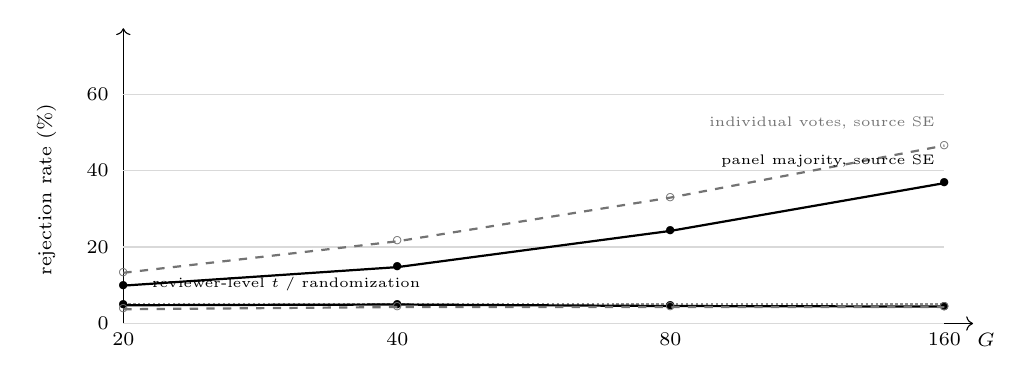
\begin{tikzpicture}[font=\scriptsize]
\draw[->] (0,0) -- (0.89\columnwidth,0) node[right, xshift=-2pt, yshift=-6pt] {$G$};
\draw[->] (0,0) -- (0,3.75cm);
\node[rotate=90, anchor=south] at (-0.06\columnwidth,1.70cm) {rejection rate (\%)};
\draw[black!15] (0,0.000cm) -- (0.86\columnwidth,0.000cm);
\node[anchor=east] at (-0.005\columnwidth,0.000cm) {0};
\draw[black!15] (0,0.971cm) -- (0.86\columnwidth,0.971cm);
\node[anchor=east] at (-0.005\columnwidth,0.971cm) {20};
\draw[black!15] (0,1.943cm) -- (0.86\columnwidth,1.943cm);
\node[anchor=east] at (-0.005\columnwidth,1.943cm) {40};
\draw[black!15] (0,2.914cm) -- (0.86\columnwidth,2.914cm);
\node[anchor=east] at (-0.005\columnwidth,2.914cm) {60};
\draw[black!45, densely dotted, thick] (0,0.243cm) -- (0.86\columnwidth,0.243cm);
\node[anchor=north] at (0.000\columnwidth,0) {20};
\node[anchor=north] at (0.287\columnwidth,0) {40};
\node[anchor=north] at (0.573\columnwidth,0) {80};
\node[anchor=north] at (0.860\columnwidth,0) {160};
\draw[black, solid, thick] (0.000\columnwidth,0.481cm) -- (0.287\columnwidth,0.716cm) -- (0.573\columnwidth,1.176cm) -- (0.860\columnwidth,1.783cm);
\node[black] at (0.000\columnwidth,0.481cm) {$\bullet$};
\node[black] at (0.287\columnwidth,0.716cm) {$\bullet$};
\node[black] at (0.573\columnwidth,1.176cm) {$\bullet$};
\node[black] at (0.860\columnwidth,1.783cm) {$\bullet$};
\draw[black!55, dashed, thick] (0.000\columnwidth,0.644cm) -- (0.287\columnwidth,1.044cm) -- (0.573\columnwidth,1.599cm) -- (0.860\columnwidth,2.260cm);
\node[black!55] at (0.000\columnwidth,0.644cm) {$\circ$};
\node[black!55] at (0.287\columnwidth,1.044cm) {$\circ$};
\node[black!55] at (0.573\columnwidth,1.599cm) {$\circ$};
\node[black!55] at (0.860\columnwidth,2.260cm) {$\circ$};
\draw[black, solid, thick] (0.000\columnwidth,0.232cm) -- (0.287\columnwidth,0.241cm) -- (0.573\columnwidth,0.222cm) -- (0.860\columnwidth,0.215cm);
\node[black] at (0.000\columnwidth,0.232cm) {$\bullet$};
\node[black] at (0.287\columnwidth,0.241cm) {$\bullet$};
\node[black] at (0.573\columnwidth,0.222cm) {$\bullet$};
\node[black] at (0.860\columnwidth,0.215cm) {$\bullet$};
\draw[black!55, dashed, thick] (0.000\columnwidth,0.181cm) -- (0.287\columnwidth,0.209cm) -- (0.573\columnwidth,0.210cm) -- (0.860\columnwidth,0.208cm);
\node[black!55] at (0.000\columnwidth,0.181cm) {$\circ$};
\node[black!55] at (0.287\columnwidth,0.209cm) {$\circ$};
\node[black!55] at (0.573\columnwidth,0.210cm) {$\circ$};
\node[black!55] at (0.860\columnwidth,0.208cm) {$\circ$};
\node[anchor=east, font=\tiny] at (0.86\columnwidth,2.06cm) {panel majority, source SE};
\node[anchor=east, font=\tiny, black!55] at (0.86\columnwidth,2.54cm) {individual votes, source SE};
\node[anchor=west, font=\tiny] at (0.02\columnwidth,0.50cm) {reviewer-level $t$ / randomization};
\end{tikzpicture}}
\caption{Null rejection rate against the number of sources $G$ at the estimated reviewer heterogeneity $\sigma_r=0.27$, with reviewer abilities redrawn each replicate. Adding sources makes the two source-level analyses steadily worse, and using individual votes instead of majority labels does not help: the defect is the unit of uncertainty, not the aggregation. The two reviewer-level analyses stay at the nominal level and are executable from released pre-aggregation votes. Table~\ref{tab:retrospective-remedies} gives the values and the corresponding power.}
\label{fig:remedy-calibration}
\end{figure}

\begin{table}[t]
\centering\footnotesize
\begin{tabular}{@{}lr@{}}
\toprule
Quantity & Value \\
\midrule
Crossed design & 3 coders $\times$ 80 claims \\
Coder accuracy vs.\ adjudicated & 0.850, 0.775, 0.725 \\
$\hat\sigma_r$ (moment estimate) & 0.271 \\
Reviewer bootstrap 95\% & [0.000, 0.347] \\
Item bootstrap 95\% & [0.000, 0.522] \\
Parametric bootstrap 95\% & [0.000, 0.732] \\
Parametric bias of $\hat\sigma_r$ & $-0.044$ \\
\midrule
\multicolumn{2}{@{}l}{\emph{Identification from published reporting}} \\
Widest admissible $\sigma_r$ set & 100\% of the grid \\
Point identified by reporting? & no \\
\bottomrule
\end{tabular}
\caption{Reviewer heterogeneity is estimable only from a crossed reviewer-by-item design, and three coders do not estimate it. All three resampling schemes are shown because they disagree about the width and not about the conclusion: every interval contains zero, so this design alone cannot distinguish a badly miscalibrated panel from a homogeneous one. The reviewer bootstrap is the scheme reported for all seven designs in Table~\ref{tab:sigma-r-anchors}, because the reviewer is the unit the parameter is about; the item bootstrap resamples the wrong unit and is shown only for comparison. A parametric bootstrap puts the estimator's bias at $-0.044$ here, against at most $0.012$ in every large design, which is what two degrees of freedom costs. The published agreement rates located in the audited papers place no usable restriction on $\sigma_r$: at the label prevalence those papers imply, every value on a $0$--$1.2$ grid reproduces the reported agreement for some item dispersion. Separating the two components requires the item-by-annotator assignment, which none of the nine audited papers reports.}
\label{tab:reviewer-heterogeneity-anchor}
\end{table}

\begin{table}[t]
\centering\footnotesize
\setlength{\tabcolsep}{1.2pt}
\begin{tabular}{@{}lrrrr@{}}
\toprule
Setting & Source & Panel RI & Rater RI & SD/SE \\
\midrule
$\sigma=0.20$, $G=20$ & 7.6 (0.4) & 4.9 (0.3) & 3.7 (0.3) & 1.14 \\
Homog., $G=80$ & 4.9 (0.3) & 4.5 (0.3) & 4.5 (0.3) & 0.99 \\
$\sigma=0.20$, $G=80$ & 17.0 (0.5) & 5.3 (0.3) & 4.6 (0.3) & 1.44 \\
$\sigma=0.20$, $G=160$ & 25.9 (0.6) & 4.9 (0.3) & 5.2 (0.3) & 1.77 \\
\bottomrule
\end{tabular}
\caption{Oracle design benchmark, retained for reference. Entries are rejection percentages with Monte Carlo standard errors in parentheses, and SD/SE is the empirical standard deviation of the D$-$C contrast divided by the mean source-only standard error, so a value above one marks an optimistic standard error. Each row uses 5,000 replicates, 12 auditors (six per prompt), six claims per source, and balanced three-of-six panels; $G$ is the number of sources and rater ability follows 12 fixed normal quantiles on the logit scale around 75\% mean agreement. Source $t$ and Panel RI use the identical studentized panel-majority statistic; Panel RI refers it to all 924 six-versus-six assignments under a full-vote oracle with an arm-independent schedule, and Rater RI uses individual accuracy. Panel RI is not implementable retrospectively, which is why Table~\ref{tab:retrospective-remedies} replaces it with two analyses that are, and evaluates them at the estimated $\sigma_r$ rather than at an assumed one. The complete null-simulation sweep, including the $\sigma_r=0.10$, $\sigma_r=0.30$ and $G=40$ profiles and the raw-contrast randomisation sensitivity, is released as \texttt{supplement/assignment\_mismatch\_simulation.json}.}
\label{tab:assignment-mismatch-simulation}
\end{table}


\FloatBarrier
\section{Crossed Deployment-Panel Details}
\label{sec:appendix-cmj}
\begin{table}[t]
\centering\small
\setlength{\tabcolsep}{4pt}
\begin{tabular}{@{}llrrrr@{}}
\toprule
Panel & Field & $N$ & $\kappa$ & $\kappa_{\max}$ & $AC_1$ \\
\midrule
Three human coders & verdict & 80 & 0.35 & 0.49 & 0.57 \\
 & C1 & 80 & 0.15 & 0.44 & 0.34 \\
 & C4 & 80 & 0.36 & 0.78 & 0.68 \\
\addlinespace
Deployed model panel (3) & verdict & 79 & 0.21 & 0.71 & 0.23 \\
 & C1 & 79 & 0.08 & 0.41 & 0.28 \\
 & C4 & 79 & 0.31 & 0.54 & 0.55 \\
\addlinespace
Second model panel (3) & verdict & 80 & -0.11 & 0.12 & 0.02 \\
 & C1 & 80 & -0.01 & 0.15 & 0.23 \\
 & C4 & 80 & -0.00 & 0.18 & 0.19 \\
\addlinespace
All model judges & verdict & 79 & 0.11 & 0.42 & 0.14 \\
 & C1 & 79 & 0.12 & 0.36 & 0.31 \\
 & C4 & 79 & 0.17 & 0.38 & 0.36 \\
\bottomrule
\end{tabular}
\caption{Reliability on the same \HumN{} published comparative claims, under the same frozen codebook. The human panel is three independently recruited coders (\HumHours{} person-hours) who were additionally instructed to open each source; the model panels read the quotation and its context. The deployed panel is the census panel of \S\ref{sec:applied} (gpt-5-mini, claude-opus-4.6, gemini-3.1-pro-preview); the second panel is a disjoint checkpoint from each of the same three developers, so the comparison does not rest on one triple. $\kappa$ is Fleiss' $\kappa$ over the panel, $\kappa_{\max}$ the Umesh ceiling those raters' own marginals permit, $AC_1$ Gwet's prevalence-robust coefficient. The second panel's near-zero $\kappa$ should be read against its ceiling of \HumFrontVerdictKmax{}, not as noise: two of its checkpoints sit at opposite ends of the threshold range (\HumModSpreadLo\%--\HumModSpreadHi\% of claims called sound), so their marginals barely overlap and almost no $\kappa$ is attainable. That is the threshold heterogeneity of \S\ref{sec:practice} in its sharpest form. Intervals in \texttt{human\_anchor\_results.json} resample sources.}
\label{tab:human-anchor}
\end{table}

\begin{table}[t]
\centering\small
\setlength{\tabcolsep}{4pt}
\begin{tabular}{@{}lrrr@{}}
\toprule
Population & $N$ & census-eligible & obs.\ agr. \\
\midrule
Published claims & 80 & 5--8\% & 0.98 \\
Screen windows & 704 & 100\% (by selection) & 0.45 \\
\bottomrule
\end{tabular}
\caption{Why the human anchor is not transferred to the census. The same three deployed judges apply the same census codebook to the \BrgClaimN{} published claims the human panel coded and to the \CensusEligible{} eligible screen windows of \S\ref{sec:applied}. Only \BrgEligLo--\BrgEligHi\% of the claims are eligible under the census rule, which demands a number credited to a different paper, so the two populations barely intersect and the high agreement in the first row is judges defaulting to one label on ineligible items, not an easier task. We therefore report the human result as evidence about adjudicating published claims and compare no $\kappa$ across the two rows.}
\label{tab:population-bridge}
\end{table}

\begin{table}[t]
\centering\footnotesize
\setlength{\tabcolsep}{1.5pt}
\resizebox{\columnwidth}{!}{%
\begin{tabular}{@{}lrrr@{}}
\toprule
Developer (models) & Probe & C2 $\Delta$ & C5 $\Delta$ \\
\midrule
01.AI (1) & +12.3 & -5.2 & +2.5 \\
AI2 (2) & +2.3 & -4.3 & -1.6 \\
Alibaba (5) & -0.2 & +10.4 & +2.1 \\
Anthropic (2) & +0.4 & -2.3 & -7.0 \\
Google (2) & +0.9 & +6.6 & -3.2 \\
HuggingFace (2) & -0.1 & +2.7 & -3.7 \\
IBM (2) & -3.9 & -1.3 & +0.1 \\
Meta (1) & -4.8 & +5.6 & -3.5 \\
Microsoft (2) & -0.4 & +10.2 & +3.1 \\
Mistral (2) & -7.0 & -0.6 & +0.0 \\
NVIDIA (1) & +1.0 & +4.7 & -2.0 \\
TII (2) & -1.8 & +1.7 & +5.0 \\
Zhipu (1) & -0.8 & -4.7 & +5.4 \\
\midrule
Pooled (random effects) & -0.4 & +3.1 & +0.1 \\
\quad 95\% CI & [-1.2, +0.4] & [+0.7, +5.5] & [-1.3, +1.5] \\
\quad 95\% pred. & [-4.4, +3.6] & [-9.8, +16.0] & [-7.2, +7.3] \\
\quad $I^2$ & 90\% & 98\% & 97\% \\
\quad dev.\ level & +0.1 & +1.7 & +0.4 \\
\bottomrule
\end{tabular}}
\caption{Controlled consequence test, \emph{full} minus \emph{placebo} in accuracy points, aggregated by developer. Checkpoints are nested in developers, so the developer-level row averages within developer before pooling. The prediction interval, not the confidence interval, is the quantity relevant to a claim about a model population; it contains zero on both substantive strata. The competence probe is the negative control. Per-model contrasts, Holm-adjusted values, paraphrase spread and the decision-normalisation report are in Appendix Table~\ref{tab:controlled-model-judges-strata-v2}.}
\label{tab:controlled-model-judges-v2}
\end{table}

\begin{table*}[t]
\centering\scriptsize
\setlength{\tabcolsep}{3pt}
\begin{tabular}{@{}llrrrrrrrr@{}}
\toprule
Model & Stratum & Abl. & Plac. & Full & F$-$P & F$-$A & Para.\ SD & McNemar $p$ & Holm $p$ \\
\midrule
Qwen2.5-14B & all & 60.9 & 59.0 & 61.6 & +2.6 & +0.7 & 3.3 & 0.008 & -- \\
Qwen2.5-14B & probe competence & 94.8 & 91.9 & 92.3 & +0.4 & -2.5 & 5.5 & 0.031 & -- \\
Qwen2.5-14B & c2 capability & 59.9 & 56.6 & 61.4 & +4.8 & +1.5 & 5.8 & 0.031 & 0.000 \\
Qwen2.5-14B & c5 utility & 44.9 & 44.9 & 46.5 & +1.6 & +1.6 & 2.4 & 0.001 & 0.068 \\
Qwen2.5-7B & all & 60.0 & 56.0 & 59.8 & +3.7 & -0.2 & 2.4 & 0.003 & -- \\
Qwen2.5-7B & probe competence & 89.2 & 85.4 & 82.1 & -3.3 & -7.1 & 8.8 & 1.000 & -- \\
Qwen2.5-7B & c2 capability & 66.1 & 59.0 & 70.1 & +11.1 & +4.0 & 7.0 & 0.000 & 0.000 \\
Qwen2.5-7B & c5 utility & 39.3 & 38.3 & 38.2 & -0.1 & -1.0 & 2.1 & 0.383 & 1.000 \\
Qwen3-14B & all & 54.1 & 54.8 & 61.3 & +6.5 & +7.2 & 4.3 & 0.000 & -- \\
Qwen3-14B & probe competence & 94.4 & 96.5 & 97.3 & +0.8 & +2.9 & 2.8 & 1.000 & -- \\
Qwen3-14B & c2 capability & 53.5 & 51.7 & 65.9 & +14.3 & +12.4 & 5.1 & 0.000 & 0.000 \\
Qwen3-14B & c5 utility & 34.5 & 37.2 & 38.8 & +1.6 & +4.3 & 5.1 & 0.002 & 0.253 \\
Qwen3-8B & all & 59.7 & 60.0 & 65.9 & +5.9 & +6.2 & 4.2 & 0.000 & -- \\
Qwen3-8B & probe competence & 69.0 & 69.2 & 70.0 & +0.8 & +1.0 & 4.0 & 1.000 & -- \\
Qwen3-8B & c2 capability & 74.0 & 74.5 & 80.5 & +6.0 & +6.6 & 7.9 & 0.016 & 0.000 \\
Qwen3-8B & c5 utility & 40.8 & 40.9 & 49.2 & +8.2 & +8.3 & 8.6 & 0.000 & 0.000 \\
OLMo-2-13B & all & 47.4 & 46.0 & 47.8 & +1.8 & +0.4 & 5.8 & 0.016 & -- \\
OLMo-2-13B & probe competence & 69.6 & 65.0 & 70.6 & +5.6 & +1.0 & 10.5 & 0.016 & -- \\
OLMo-2-13B & c2 capability & 50.7 & 48.3 & 53.1 & +4.8 & +2.4 & 3.1 & 0.000 & 0.000 \\
OLMo-2-13B & c5 utility & 32.9 & 34.2 & 31.0 & -3.1 & -1.9 & 9.2 & 0.021 & 0.000 \\
OLMo-2-7B & all & 41.5 & 40.2 & 41.7 & +1.4 & +0.1 & 7.8 & 0.500 & -- \\
OLMo-2-7B & probe competence & 43.1 & 48.1 & 44.8 & -3.3 & +1.7 & 4.5 & 0.500 & -- \\
OLMo-2-7B & c2 capability & 44.8 & 46.9 & 44.3 & -2.6 & -0.5 & 5.5 & 1.000 & -- \\
OLMo-2-7B & c5 utility & 37.5 & 29.7 & 37.5 & +7.8 & +0.0 & 15.6 & 1.000 & -- \\
Granite-3.1-8B & all & 53.8 & 54.8 & 53.7 & -1.2 & -0.1 & 2.3 & 0.011 & -- \\
Granite-3.1-8B & probe competence & 81.9 & 85.2 & 78.1 & -7.1 & -3.7 & 7.7 & 0.003 & -- \\
Granite-3.1-8B & c2 capability & 55.9 & 56.4 & 57.6 & +1.2 & +1.7 & 3.5 & 1.000 & 0.200 \\
Granite-3.1-8B & c5 utility & 37.5 & 38.1 & 37.5 & -0.6 & +0.0 & 0.7 & 1.000 & 0.213 \\
Phi-4-mini & all & 61.5 & 60.8 & 62.0 & +1.2 & +0.5 & 0.7 & 0.000 & -- \\
Phi-4-mini & probe competence & 67.3 & 69.4 & 69.8 & +0.4 & +2.5 & 7.5 & 1.000 & -- \\
Phi-4-mini & c2 capability & 75.8 & 73.2 & 74.0 & +0.7 & -1.9 & 4.7 & 0.024 & 1.000 \\
Phi-4-mini & c5 utility & 44.2 & 44.0 & 46.0 & +2.1 & +1.9 & 2.1 & 0.000 & 0.213 \\
Falcon3-7B & all & 58.4 & 58.1 & 59.1 & +1.0 & +0.7 & 2.1 & 0.860 & -- \\
Falcon3-7B & probe competence & 66.7 & 66.7 & 66.7 & +0.0 & +0.0 & 0.0 & 1.000 & -- \\
Falcon3-7B & c2 capability & 68.8 & 68.3 & 69.0 & +0.6 & +0.2 & 1.2 & 1.000 & 0.901 \\
Falcon3-7B & c5 utility & 44.0 & 43.5 & 45.5 & +2.0 & +1.6 & 4.3 & 0.678 & 0.302 \\
\bottomrule
\end{tabular}
\caption{Per-model, per-stratum results for the version-2 controlled experiment. Accuracies are percentages averaged over four paraphrases; F$-$P and F$-$A are the full-minus-placebo and full-minus-ablated contrasts in percentage points; \emph{Para.\ SD} is the standard deviation of the full-minus-placebo contrast across paraphrases. McNemar tests use per-item paraphrase-majority decisions. Holm adjustment covers gate-passing models on the two substantive strata.}
\label{tab:controlled-model-judges-strata-v2}
\end{table*}


\FloatBarrier
\section{Framework Details and Positioning}
\begin{figure*}[t]
\centering
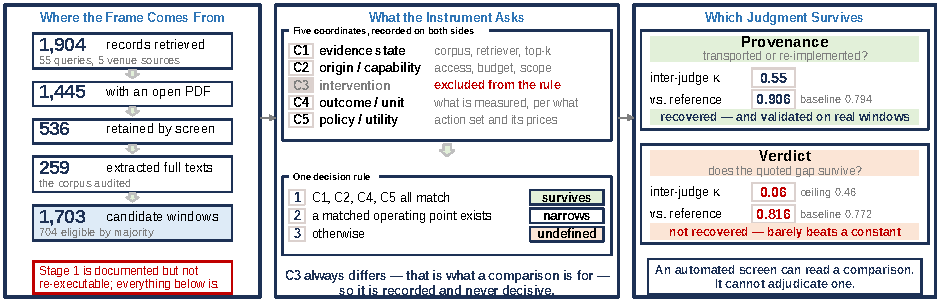
\includegraphics[width=\textwidth]{figures/generated/fig_instrument.pdf}%
\caption{The taxonomy as an instrument. \emph{Left:} the documented screening
flow from retrieval to the \FlowTexts{} extracted full texts the survey reads
and the audit runs over. \emph{Middle:} the five coordinates and the one
decision rule they feed, with the intervention coordinate recorded but excluded.
\emph{Right:} which of the instrument's two judgments survives contact with
published text.}
\label{fig:instrument}
\end{figure*}

\begin{figure}[t]
\centering
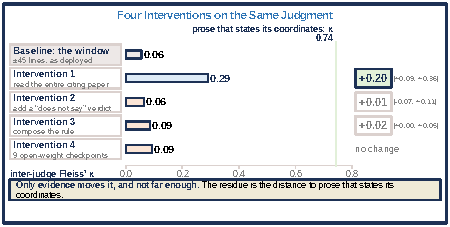
\includegraphics[width=\columnwidth]{figures/generated/fig_interventions.pdf}%
\caption{Why adjudication is not recoverable, established by intervention rather
than by inference. Judges, codebook and items are held fixed and one thing is
varied at a time. Only supplying the papers themselves moves inter-judge
agreement, and it stops well short of the level the same instrument reaches on
prose written to state its coordinates.}
\label{fig:interventions}
\end{figure}

% Drawn by scripts/revision3/fig_appendix_flows.py; the .pptx is the editable
% source and is released with the paper.
\begin{figure}[t]
\centering
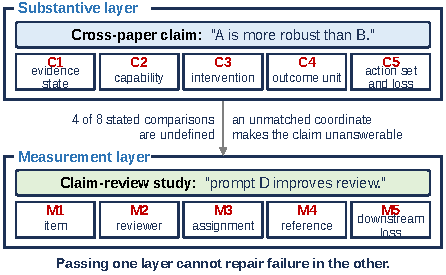
\includegraphics[width=\columnwidth]{figures/generated/fig_two_layer.pdf}%
\caption{The two layers answer different questions about the same sentence.
The substantive layer asks whether two published results concern one decision
problem; Table~\ref{tab:cross-paper-cases} applies it to real comparisons and
supplies the four-of-eight count. The measurement layer asks what a study of
claim review estimates; Table~\ref{tab:retrospective-remedies} shows which
analyses of such a study are valid. Passing one layer cannot repair failure in
the other.}
\label{fig:two-layer}
\end{figure}

\begin{table*}[t]
\centering
\footnotesize
\renewcommand{\arraystretch}{0.92}
\begin{tabularx}{\linewidth}{>{\raggedright\arraybackslash}p{0.18\linewidth}>{\raggedright\arraybackslash}p{0.22\linewidth}>{\raggedright\arraybackslash}p{0.25\linewidth}X}
\toprule
\textbf{Adjacent line} & \textbf{Primary unit} &
\textbf{Unresolved comparison question} & \textbf{This paper's increment} \\
\midrule
General RAG surveys \citep{ragSurvey2024,ragComprehensive2025} &
Architectures, modules, applications &
Whether similarly named gains concern the same evidence state, outcome, and
experimental game &
Adds a claim-level comparison lens and an estimand audit; does not claim a
venue-complete census. \\
Evaluation surveys and unified comparisons
\citep{ragEvaluationSurvey2024,ragBestPractices2024,
alushiRAGComparison2026} &
Metrics, benchmarks, and common-harness reruns &
Which controls are required by a specific cross-study or mechanistic
inference when rerunning is impossible &
Separates scientific coordinates from assignment, participant, item, and
reference units; the simulation quantifies one resulting failure mode. \\
Trustworthy and security RAG surveys
\citep{trustRAGCompass2024,trustworthyRAGSurvey2025,securityRAGSurvey2026} &
Trust dimensions, attack surfaces, and defenses &
Whether benign conflict and attacker-created corruption share a transferable
capability envelope &
Makes origin/access/budget explicit and shows why a prompt-overlapping
reference cannot establish independent criterion validity. \\
Conflict and abstention surveys
\citep{xuKnowledgeConflicts2024,wenAbstentionSurvey2025} &
Conflict types and refusal behavior &
Whether a confidence or sufficiency signal identifies the action that
maximizes utility at a matched operating point &
Separates signal, action, and utility and releases a consequence-defined
counterfactual target without claiming an evaluated policy. \\
\bottomrule
\end{tabularx}
\caption{Positioning relative to adjacent surveys and empirical comparison
work. Each adjacent line partitions the literature by mechanism, which is what a
reader needs to \emph{find} related work. None partitions the
\emph{comparison}, which is what a reader needs when two numbers appear
together, and none is accompanied by evidence that its categories can be read
off a paper. The increment is a reporting-coordinate reduction that is tested
(\S\ref{sec:tested}) and applied at scale (\S\ref{sec:applied}); it is not a
venue-complete systematic review, and it does not supersede these surveys for
discovery.}
\label{tab:main-prior-work-comparison}
\end{table*}

\begin{table*}[t]
\centering
\small
\renewcommand{\arraystretch}{0.92}
\begin{tabularx}{\linewidth}{>{\raggedright\arraybackslash}p{0.13\linewidth}>{\raggedright\arraybackslash}p{0.25\linewidth}>{\raggedright\arraybackslash}p{0.30\linewidth}X}
\toprule
\textbf{Field} & \textbf{Question} & \textbf{Representative values} & \textbf{Why it changes a comparison} \\
\midrule
Evidence state & What is observable at the decision boundary? & Supported; distracting; insufficient; conflicting; stale/weak provenance; adversarially manipulated; not evidence-conditioned. & Query ambiguity and model uncertainty are not silently mixed with properties of retrieved evidence. \\
Origin / capability & How did that state arise, and what can an attacker observe or change? & Benign retrieval; constructed stressor; natural drift/conflict; distribution shift; attacker-created evidence with access, budget, and target. & Transfer depends on the data-generating process and the attacker's capability envelope. \\
Intervention & What part of the system changes? & Corpus/index; retriever; reranker; context assembly; generator; verifier; system control; evaluation artifact. & Components may be alternatives in a shared harness or complementary stages in a pipeline. \\
Outcome & What object and unit are measured? & Answer correctness; retrieval quality; claim support; attack success; privacy leakage; calibration; selective risk; cost. & Identically named datasets do not make different target quantities interchangeable. \\
\textbf{Policy / utility} & What response is selected, under which costs and stakes? & Answer; verify; re-retrieve; expose conflict; clarify; quarantine; recover; abstain; coverage--risk utility. & A signal becomes operational only through an action set and a declared utility context. \\
\midrule
Control check & Does the experiment support the intended inference? & Dataset and corpus snapshot; retriever; top-$k$; generator; decoding; budget; baselines; uncertainty. & Tuple compatibility alone cannot remove experimental confounding. \\
\bottomrule
\end{tabularx}
\caption{The diagnostic schema. The five fields identify whether two results address a compatible question; a claim-specific control check then determines whether their reported numbers support the intended inference. The fields are not assumed orthogonal or sufficient.}
\label{tab:main-framework-overview}
\end{table*}

\begin{table*}[t]
\centering
\scriptsize
\renewcommand{\arraystretch}{0.88}
\begin{tabularx}{\linewidth}{>{\raggedright\arraybackslash}p{0.13\linewidth}>{\raggedright\arraybackslash}p{0.26\linewidth}>{\raggedright\arraybackslash}p{0.30\linewidth}X}
\toprule
\textbf{Coordinate} & \textbf{Controlled values} & \textbf{Equivalence / boundary rule} & \textbf{Verdict effect} \\
\midrule
Evidence state & Supported; irrelevant/distracting; insufficient; conflicting; stale/weak provenance; adversarially manipulated; not evidence-conditioned. & Code what is observable at the decision boundary. Query ambiguity, OOD input, confidence, and attacker access are not evidence states by themselves. & A direct performance claim normally requires a common state or an explicit cross-state estimand. \\
Origin / capability & Benign retrieval; constructed stressor; natural conflict/drift; query or distribution shift; attacker-created evidence; shared clean harness. & Record how the state arose. For security, include corpus write access, query control, retriever visibility, generator access, insertion budget, objective, and target. & A cross-source rank over two different games narrows at best and is otherwise undefined; a shared harness may deliberately vary capability as the controlled factor. \\
Intervention point & Corpus/index; retriever; reranker; context assembly/compression; generator prompting or training; verifier; system-control policy; evaluation-only artifact. & Code the component changed. Different interventions may be compared as alternatives when a shared end-to-end harness controls the remaining pipeline; otherwise they provide component-specific or compositional evidence. & C3 never enters the decision rule. Comparing two different systems means the intervention differs, so a C3 mismatch is the normal state of a comparison and cannot by itself make one undefined; it is recorded so a reader knows what changed. \\
Outcome / unit & Answer correctness; retrieval quality; evidence support; attack or defense utility; privacy leakage; calibration; selective risk/coverage; cost/latency; human preference. & Record definition, direction, aggregation, and unit. Relative gains over different baselines are not automatically a shared estimand. & A one-scalar ranking requires a common target. Without one there is no operating point to re-read at, so the gap is undefined rather than narrowed. \\
Policy / utility & Answer; abstain; re-retrieve; filter; verify; expose conflict; clarify; quarantine; recover; not applicable; unreported. & Use \emph{not applicable} for fixed descriptive comparisons. When policies compete, report action set, stakes, preferences, coverage, and cost. & Different actions can be ranked only under common utility; a signal alone does not establish the preferred response. A stated price at the other side's setting narrows the comparison. \\
Second-stage controls & Dataset/corpus snapshot; retriever/top-$k$/chunking; generator/decoding; compute budget; baselines; uncertainty/statistical design. & Select controls according to the stated inference. The tuple cannot remove confounding from unmatched experimental systems. & Tuple compatibility is necessary diagnostic information but not sufficient for a direct empirical ranking. \\
Final verdict & Survives; narrows; undefined. & Exactly the rule of \S\ref{sec:estimands}, and the only verdict vocabulary used anywhere in this paper or its artifacts. \emph{Survives}: C1, C2, C4 and C5 all match, so the quoted gap stands. \emph{Narrows}: a threatening coordinate differs but a side reports an operating point at the other's setting, or the comparison holds on a strict subset; report that matched number. \emph{Undefined}: no such operating point exists, or a decision-critical field is unavailable after full-text inspection. & Verdicts attach to comparison claims, not permanently to paper pairs, and a new shared-harness experiment can change the supported verdict. An undefined comparison is never replaced by a substitute number computed across the unmatched coordinate. \\
\bottomrule
\end{tabularx}
\caption{The decision procedure of \S\ref{sec:estimands} in full. The five coordinates diagnose semantic compatibility and claim-specific controls determine whether the claim as written is warranted, but only C1, C2, C4 and C5 enter the verdict: C3 is the thing being compared and is recorded rather than tested. The three verdicts here are the same three used in the body, the census codebook and every released artifact.}
\label{tab:framework-decision-procedure}
\end{table*}

\begin{table*}[t]
\centering
\scriptsize
\renewcommand{\arraystretch}{0.9}
\begin{tabularx}{\linewidth}{>{\raggedright\arraybackslash}p{0.20\linewidth}>{\raggedright\arraybackslash}p{0.24\linewidth}>{\raggedright\arraybackslash}p{0.24\linewidth}X}
\toprule
\textbf{Boundary case} & \textbf{Five-coordinate diagnosis} & \textbf{Second-stage control check} & \textbf{Supported conclusion} \\
\midrule
Different interventions, shared harness & A retriever filter and a generator-side reader address the same evidence state, metric target, and answer policy; intervention differs. & Same corpus, retriever output before intervention, generator, budget, metric, and seeds. & A valid end-to-end comparison is possible. Intervention mismatch alone does not force \emph{partial}. \\
All five fields match, systems differ & Two answer-only methods target benign retrieval noise and answer correctness at the generator. & Different datasets, retrievers, model scales, top-$k$, and compute budgets. & The papers are conceptually comparable but their reported numbers are not directly rankable without a shared rerun or adjustment. \\
Action unnamed but observable & A QA benchmark never uses ``action policy'' but requires one answer for every item and gives no abstention channel. & Evaluation code and output schema confirm answer-only behavior. & Code \emph{answer} when policy is decision-relevant; use \emph{not applicable} for a fixed descriptive comparison. \\
Same pair, different claim & An attack artifact and a defense share a threat model but optimise attack success and defended utility. & A common attack--defense harness can evaluate both roles; a paper-only scalar comparison cannot. & Valid as components of one evaluation, partial as substitutable methods, invalid if ranked under incompatible objectives. \\
Same label, incompatible capability & Two poisoning studies both report attack success, but one assumes bounded corpus insertion and the other controls retrieved instructions at query time. & Capability, budget, retrieval probability, and objective do not align. & A direct ranking is invalid even if intervention, metric name, and answer behavior appear similar. \\
\bottomrule
\end{tabularx}
\caption{Counterexamples delimiting the schema. Verdicts depend on the stated comparison and experimental controls; the five coordinates are diagnostic fields rather than a necessary-and-sufficient classifier.}
\label{tab:framework-counterexamples}
\end{table*}


\FloatBarrier
\section{Reporting Checklist}
\label{sec:appendix-eval}
\begin{table*}[t]
\centering
\scriptsize
\renewcommand{\arraystretch}{0.9}
\begin{tabularx}{\linewidth}{>{\raggedright\arraybackslash}p{0.18\linewidth}>{\raggedright\arraybackslash}p{0.30\linewidth}>{\raggedright\arraybackslash}p{0.22\linewidth}X}
\toprule
\textbf{Required field} & \textbf{What to report} & \textbf{If omitted} & \textbf{Example consequence} \\
\midrule
Evidence-state definition & Supported, irrelevant/distracting, insufficient, conflicting, stale/weak provenance, adversarially manipulated, or not evidence-conditioned. & Papers with the same robustness label may test different evidence properties. & Noise training is ranked against sufficiency prediction. \\
Origin / capability & Benign retrieval, constructed stressor, natural conflict/drift, distribution shift, or attacker access, budget, objective, and target. & Stressors are not portable. & Natural conflict is compared with poisoning. \\
Intervention boundary & Corpus/KB, retriever/context, context assembly, generator, system control, or evaluation artifact. & Pipeline modules are treated as substitutable. & A benchmark is ranked against a mitigation method. \\
Retrieval setting & Corpus snapshot, retriever, top-$k$, chunking, reranking/compression, and index drift controls. & Results cannot be reproduced or normalised. & A filter looks better because its retriever retrieved easier negatives. \\
Outcome and unit & Answer correctness, support, attack success, privacy leakage, selective risk, calibration, cost, or action utility, including definition and aggregation. & Different objectives collapse into one score. & Lower attack success hides clean-utility loss. \\
Policy and utility & Answer, abstain, retrieve again, filter, verify, expose conflict, clarify, quarantine, or recover, plus stakes, preferences, coverage, and cost when actions compete. & Accuracy and confidence are over-interpreted. & A calibrated answerer may still answer from insufficient evidence. \\
Model and comparison controls & Dataset, generator, decoding, compute budget, baselines, seeds, uncertainty intervals, and significance procedure. & Tuple-aligned papers can still be empirically confounded. & A method appears better because it uses a stronger generator or a larger budget. \\
Uncertainty / abstention handling & Coverage, selective risk, confidence target, abstention reward, and re-retrieval cost. & Abstention can hide retrieval failure. & Refusal is rewarded when re-retrieval should be the correct action. \\
Security threat model & Attacker access, query control, retriever visibility, insertion budget, objective, and adaptive-defense assumptions. & Security numbers are not comparable. & Prompt injection defenses are claimed to protect against corpus poisoning. \\
\midrule
Provenance of every quoted number & Whether the other side's figure was \emph{transported} from its paper or \emph{re-implemented} in this harness, and at which configuration. & The one property an automated audit recovers reliably ($\kappa$ \DecProvK{}) is lost, and the stratum where incomparability lives cannot be found. & A re-implementation at a strengthened attack budget reads as a defeat of the published attack. \\
Reviewer/judge panel and unit map & Who or what adjudicated, how many, which items each saw, and how any prompt or instruction was assigned across them. & The unit of assignment is unrecoverable, so uncertainty cannot be computed at the unit that was varied. & A source-level test rejects a true null $\SimAtCensus\%$ of the time at the heterogeneity measured here. \\
Pre-aggregation votes & Per-reviewer labels with stable reviewer identifiers, before adjudication or majority voting. & Only reviewer-level analyses hold their nominal size, and they need these votes. & A reported agreement rate cannot be converted into a valid reviewer-level test after the fact. \\
\bottomrule
\end{tabularx}
\caption{Reporting checklist for robust RAG under unreliable evidence, in the order of \S\ref{sec:practice}. The first block is the five coordinates and the controls that accompany them. \S\ref{sec:instrument} shows why they head the list: a comparison whose answer turns on a coordinate the paper does not state is the one case in which a panel neither agrees nor is right, and C1 and C4 are the two fields whose absence produces that case most often. The last block is what the audit of the audit requires.}
\label{tab:robust-rag-reporting-checklist}
\end{table*}


\FloatBarrier
\section{Scoping-Map Audit Artifacts}
\label{sec:audit-artifacts}
\begin{table*}[t]
\centering
\small
\renewcommand{\arraystretch}{0.95}
\begin{tabularx}{\linewidth}{>{\raggedright\arraybackslash}p{0.16\linewidth}>{\raggedright\arraybackslash}p{0.19\linewidth}>{\raggedright\arraybackslash}p{0.25\linewidth}>{\raggedright\arraybackslash}X}
\toprule
\textbf{Evidence layer} & \textbf{Unit and size} & \textbf{Structured coverage} & \textbf{Supported use and provenance boundary} \\
\midrule
Scoping corpus & 536 broadly included papers & Metadata and broad relevance & Documentary recall pool; single model-assisted broad screen, not duplicated and not prevalence-estimating. \\
Map B & 342 paper rows & Literature family and intervention; free-text metrics; no structured evidence origin or policy & Source-stratified landscape synthesis; adjudicated subsets, but not a five-coordinate map. \\
Claim inventory & 289 claims from purposive fixed sections & Model-coded coordinates, evidence flags, and claim-specific controls & Source-linked hypothesis index; its verdict distribution and internal ablations are not validated results. \\
Instrument benchmark & 360 constructed comparability items & Five coordinate values and a verdict fixed when each item is written; six judges from three developers under three codebooks & The instrument claim of \S\ref{sec:instrument}. Templated prose, so it bounds what the schema can do on text that states it, not on any particular published passage. \\
Cross-paper census & 1,703 frame windows & Nine judges, fully crossed, one codebook & The prevalence and reliability claims of \S\ref{sec:census}. No verdict-based rate is an estimate. \\
\bottomrule
\end{tabularx}
\caption{The released evidence layers answer different questions. Larger
model-assisted layers do not validate claim-level verdicts; the human layers
test an annotation procedure rather than literature prevalence. No layer is
treated as an independently validated gold standard.}
\label{tab:main-evidence-layers}
\end{table*}

% Drawn by scripts/revision3/fig_appendix_flows.py; the .pptx is the editable
% source and is released with the paper.
\begin{figure*}[t]
\centering
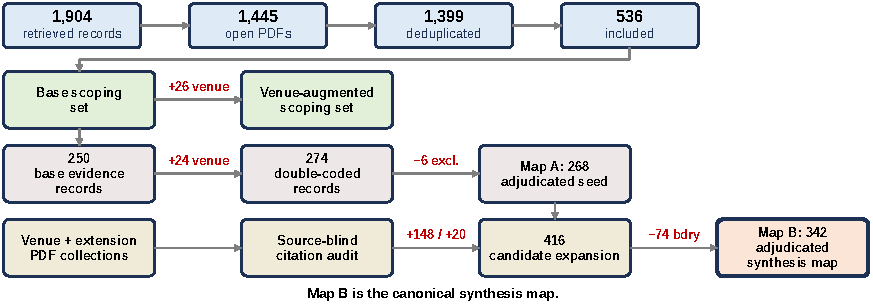
\includegraphics[width=\textwidth]{figures/generated/fig_corpus_lineage.pdf}%
\caption{Corpus lineage. Red deltas on the connectors are, in order, $+26$ and
$+24$ venue-linked additions, $-6$ exclusions, $+148$ new and $+20$ enriched
rows from the citation audit, and $-74$ boundary rows removed at adjudication.
The 416-row venue-expanded candidate map is second-coded and adjudicated into
Map~B (342 rows), the canonical synthesis evidence map. Map~A (268 rows) is the
double-coded adjudicated seed used for IAA and adjudication audit; the base and
venue-augmented scoping sets are used only for boundary checks, while a separate
300-paper source-blind citation audit over the venue and extension PDF
collections decides which papers enter the main text, case studies, or
appendix.}
\label{fig:corpus-flow}
\end{figure*}

\begin{table*}[t]
\centering
\small
\begin{tabularx}{\linewidth}{p{0.18\linewidth}p{0.16\linewidth}X}
\toprule
\textbf{Stage} & \textbf{Count} & \textbf{Rule} \\
\midrule
Initial retrieval & 1,904 records & Keyword search over arXiv, ACL Anthology, OpenReview, USENIX, AAAI/ACM landing pages where open versions were available, plus curated robust/trustworthy RAG paper lists; search cutoff 2026-06-03. \\
Open full-text corpus & 1,445 PDFs & Downloaded only open PDFs; removed failed downloads, inaccessible files, and non-PDF artifacts. \\
Deduplicated candidates & 1,399 papers & Deduplicated by normalised title and arXiv/proceedings identifiers; retained the most complete metadata record when preprint and proceedings versions overlapped. \\
Relevance screening & 536 included papers & Included papers that study RAG robustness, reliability, uncertainty, calibration, faithfulness, attack/defense, or evaluation under unreliable evidence; excluded application-only RAG papers. \\
Core pool & 112 papers & Papers directly shaping the taxonomy, threat/failure model, intervention mechanisms, or evaluation framework. \\
Core reading set & 100 papers & Core papers used as main narrative anchors; the remaining 12 core-pool papers stay in the broader scoping set. \\
Base scoping set & 300 papers & Core papers plus representative supporting work across all taxonomy branches before venue follow-up triage. \\
Venue-augmented scoping set & 326 papers & Base scoping set plus 26 venue-linked additions after follow-up triage. \\
Candidate evidence records & 274 papers & Base evidence map of 250 papers plus 24 venue-linked additions, double-coded and adjudicated. \\
Map A adjudicated seed & 268 papers & Candidate evidence records retained after final adjudication; used for IAA/adjudication provenance. \\
Map-B candidate expansion & 416 papers & Map A plus 148 source-blind human-citation-audit additions and 20 enriched original rows; used for second-coding review. \\
Map B adjudicated synthesis map & 342 papers & Map A plus 74 retained additions after second coding and final adjudication; frozen for current descriptive statistics. Post-freeze discoveries enter a recall log until a new version is coded. \\
\bottomrule
\end{tabularx}
\caption{Screening-flow summary. Search ends on 2026-06-03; coding and adjudication artifacts freeze on 2026-06-15. The supplement provides query strings, source counts, rules, exclusions, hashes, and a post-freeze recall log.}
\label{tab:review-protocol}
\end{table*}

\begin{table*}[t]
\centering
\scriptsize
\renewcommand{\arraystretch}{0.92}
\begin{tabularx}{\linewidth}{>{\raggedright\arraybackslash}p{0.20\linewidth}>{\raggedright\arraybackslash}p{0.15\linewidth}>{\raggedright\arraybackslash}p{0.30\linewidth}X}
\toprule
\textbf{Artifact / set} & \textbf{Count} & \textbf{Count definition} & \textbf{Use in this paper} \\
\midrule
Map-A double-coded candidates & 274 & Candidate records coded by two human sources before final inclusion adjudication. & Used for human-human agreement and adjudication; six records were excluded from Map A. \\
Map A adjudicated seed & 268 & Included records after adjudication: 42 venue/proceedings-linked, 222 arXiv-only or emerging preprints, 2 preprints with year tags, 1 review-platform record, and 1 other/uncategorized record. & Used as the IAA/adjudication provenance snapshot, not the current synthesis denominator. \\
Venue-augmented scoping set & 326 & Original base scoping set plus 26 triaged venue-linked additions. & Used for broader scoping and boundary checks; not all rows are evidence-map records. \\
Source-blind citation audit & 300 & Human citation decisions over venue PDFs and extension PDFs. & Determines which audited papers enter the main text, case studies, appendix, background, or exclusion set; distinct from the base scoping set. \\
Map-B candidate expansion & 416 & Map A plus 148 candidate additions supported by the source-blind citation audit; 20 original rows enriched with citation-audit metadata. & Pre-adjudication expansion candidate map used for second-coding review. \\
Map B adjudicated synthesis map & 342 & Map A plus 74 retained additions after second coding and final adjudication. & Current evidence map for source-stratified synthesis and Map-B cross-tabs. \\
\bottomrule
\end{tabularx}
\caption{Reconciliation of reported corpus counts. The 342-row adjudicated Map B is the canonical synthesis map; Map A and the 274-candidate set are retained to report double-coding and adjudication provenance.}
\label{tab:source-strata-reconciliation}
\end{table*}


\FloatBarrier
\end{document}
